% arara: xelatex: { synctex: on, shell: off }
% arara: xelatex: { synctex: on, shell: off }
% arara: biber
% arara: xelatex: { synctex: on, shell: off }
% arara: sumatrapdf
\documentclass[12pt]{report}

%Skip preambles in chapter documents
\usepackage{standalone}

\includeonly{%
chapters/01-Introduction,
chapters/02-Experimental-Facilities,
chapters/03-Butanol,
chapters/04-Pentanol,
chapters/05-MCH,
chapters/06-Conclusions}

%Set the document font
\usepackage{fontspec}
\setromanfont{Times New Roman}

%Set the size of the margins and the paper
\usepackage[margin=1in, letterpaper]{geometry}

%Set the color of the links and PDF metadata
\usepackage[
    colorlinks=true,
    citecolor=blue,
    linkcolor=black,
    pdftitle={High Pressure Ignition Chemistry of Alternative Fuels},
    pdfauthor={Bryan W. Weber}
]{hyperref}

%Set up the page numbers
%This has to go after geometry so the page number is centered
\usepackage{fancyhdr}
\pagestyle{fancy}
\fancyhf{}
\fancyfoot[C]{\thepage}
\renewcommand{\headrulewidth}{0pt}

%Set a command to easily skip a line
\newcommand{\blankline}{\vspace*{\baselineskip}}

%Set up biblatex
\usepackage[
    backend=biber,
    url=false,
    doi=true,
    sorting=none,
    sortcites=true,
    maxnames=6,
    minnames=6,
    citestyle=numeric-comp,
    firstinits=true,
    isbn=false
]{biblatex}
\addbibresource{library.bib}

%Remove the "In:" from before the journal title for articles
\renewbibmacro{in:}{%
  \ifentrytype{article}{}{\printtext{\bibstring{in}\intitlepunct}}}

%Set the sort order of the names in each bibliography entry
\DeclareNameAlias{default}{last-first}

%Don't print the article title. To print the title, add #1 to the last {}
\DeclareFieldFormat[article,incollection,unpublished]{title}{}

%Add Vol. and No. before volume and issue.
\DeclareFieldFormat[article]{volume}{\bibstring{volume}\addspace #1}
\DeclareFieldFormat[article]{number}{\bibstring{number}\addspace #1}

%Put a comma between the volume and issue instead of period
\renewbibmacro*{volume+number+eid}{%
  \printfield{volume}%
  \setunit{\addcomma\space}%<---- was \setunit*{\adddot}%
  \printfield{number}%
  \setunit{\addcomma\space}%
  \printfield{eid}}

%Add a comma after the journal title
\renewbibmacro*{journal+issuetitle}{%
  \usebibmacro{journal}%
  \setunit*{\addcomma\addspace}%
  \iffieldundef{series}
    {}
    {\newunit
     \printfield{series}%
     \setunit{\addspace}}%
  \usebibmacro{volume+number+eid}%
  \setunit{\addspace}%
  \usebibmacro{issue+date}%
  \setunit{\addcolon\space}%
  \usebibmacro{issue}%
  \newunit}

%Use the titling package to allow easy access to custom title pages
\usepackage{titling}
\title{High Pressure Ignition Chemistry of Alternative Fuels}
\author{Bryan William Weber}

%Set the text to double spacing
\usepackage[doublespacing]{setspace}

%Begin the document
\begin{document}
\thispagestyle{empty}
\begin{center}
\thetitle \\
\theauthor, Ph.D. \\
University of Connecticut, 2014 \\
\blankline
\end{center}
Abstract

\newpage

\thispagestyle{empty}
\begin{center}
\blankline \blankline 
\thetitle \\
\blankline
\theauthor \\
\blankline \blankline
B.S., Case Western Reserve University, 2009 \\
M.S., University of Connecticut, 2010 \\
\blankline \blankline \blankline \blankline \blankline \blankline
\blankline \blankline
A Dissertation \\
Submitted in Partial Fulfillment of the \\
Requirements for the Degree of Doctor of Philosophy \\
at the \\
University of Connecticut \\
\blankline \blankline
2014
\end{center}
\newpage

\thispagestyle{empty}
\begin{center}
Copyright \copyright 2014 Bryan William Weber \\

\includegraphics{images/CC-license.png} \\
\blankline
This work is licensed under a Creative Commons Attribution-NonCommercial-NoDerivatives 4.0 International License. \\
\url{http://creativecommons.org/licenses/by-nc-nd/4.0/deed.en_US} \\
\blankline \blankline \blankline \blankline \blankline \blankline
\blankline \blankline \blankline \blankline \blankline \blankline
\blankline \blankline \blankline \blankline \blankline \blankline
\blankline \blankline
2014
\end{center}
\newpage

\setcounter{page}{1}
\pagenumbering{roman}
\begin{center}
APPROVAL PAGE \\
Doctor of Philosophy Dissertation \\
\thetitle \\
\blankline \blankline
Presented by \\
\theauthor, B.S., M.S. \\
\end{center}
\blankline
\makebox[0.9\textwidth]{Major Advisor\enspace\hrulefill}
\vspace{-0.5\baselineskip}
\begin{center}
Chih-Jen Sung
\end{center}
\blankline
\makebox[0.9\textwidth]{Associate Advisor\enspace\hrulefill}
\vspace{-0.5\baselineskip}
\begin{center}
Baki Cetegen
\end{center}
\blankline
\makebox[0.9\textwidth]{Associate Advisor\enspace\hrulefill}
\vspace{-0.5\baselineskip}
\begin{center}
Michael Renfro
\end{center}
\blankline \blankline \blankline \blankline \blankline
\begin{center}
University of Connecticut \\
2014
\end{center}
\newpage

\phantomsection
\addcontentsline{toc}{chapter}{Acknowledgements} 
\chapter*{Acknowledgements}
So long, and thanks for all the fish.
\newpage

\tableofcontents
\newpage
%\listoffigures
%\newpage
%\listoftables
%\newpage

\setcounter{page}{1}
\pagenumbering{arabic}

%Introduction
% arara: xelatex: { synctex: on, shell: off }
% arara: biber
% arara: xelatex: { synctex: on, shell: off }
% arara: sumatrapdf
\documentclass[12pt, letterpaper]{article}

%Set the package to import preambles
\usepackage{subfiles}

%Load graphicx here to specify options
\usepackage[final]{graphicx}

%Set the document font
\usepackage[no-math]{fontspec}
\setmainfont[Ligatures=TeX]{Times New Roman}
\setmonofont{Inconsolata}

%Set the text to double spacing
%According to hyperref README,
%setspace should be loaded first
\usepackage[doublespacing]{setspace}

%Set a command to easily skip a line
\newcommand{\blankline}{\vspace*{\baselineskip}}

%Set up biblatex
\usepackage[
    backend=biber,
    % url=false,
    doi=true,
    sorting=none,
    sortcites=true,
    maxbibnames=6,
    minbibnames=6,
    maxcitenames=2,
    mincitenames=1,
    citestyle=numeric-comp,
    firstinits=true,
    isbn=false
]{biblatex}
\addbibresource{C:/Users/\user/Documents/Github/dissertation/library.bib}

%Remove the "In:" from before the journal title for articles
\renewbibmacro{in:}{%
  \ifentrytype{article}{}{\printtext{\bibstring{in}\intitlepunct}}}

%Change the name of the bibliography section to "References"
\DefineBibliographyStrings{english}{bibliography = {References}}

%Set the sort order of the names in each bibliography entry
\DeclareNameAlias{default}{last-first}

%Don't print the article title. To print the title, add #1 to the last {}
\DeclareFieldFormat[article,incollection,unpublished]{title}{}

%Add "vol." and "no." before volume and issue.
\DeclareFieldFormat[article]{volume}{\bibstring{volume}\addspace #1}
\DeclareFieldFormat[article]{number}{\bibstring{number}\addspace #1}

%Ensure that a comma follows abbreviated journal titles.
\DeclareFieldFormat{journaltitle}{\mkbibemph{#1}\isdot}

%Put a comma between the volume and issue instead of period.
\renewbibmacro*{volume+number+eid}{%
  \printfield{volume}%
  \setunit{\addcomma\space}%<---- was \setunit*{\adddot}%
  \printfield{number}%
  \setunit{\addcomma\space}%
  \printfield{eid}}

%Add a comma after the journal title.
\renewbibmacro*{journal+issuetitle}{%
  \usebibmacro{journal}%
  \setunit*{\addcomma\addspace}%<---- was \setunit*{\addspace}%
  \iffieldundef{series}
    {}
    {\newunit
     \printfield{series}%
     \setunit{\addspace}}%
  \usebibmacro{volume+number+eid}%
  \setunit{\addspace}%
  \usebibmacro{issue+date}%
  \setunit{\addcolon\space}%
  \usebibmacro{issue}%
  \newunit}

%Only print URL if doi is not present.
\DeclareFieldFormat{url}{%
  \iffieldundef{doi}{%
    \mkbibacro{URL}\addcolon\space\url{#1}%
  }{%
  }%
}
\DeclareFieldFormat{urldate}{%
  \iffieldundef{doi}{%
    \mkbibparens{\bibstring{urlseen}\space#1}%
  }{%
  }%
}

%Remove publisher from being printed.
\renewbibmacro*{publisher+location+date}{%
  \printlist{location}%
  \setunit*{\addcomma\space}%
  \usebibmacro{date}%
  \newunit}

%Fix in-text full citations
\DeclareCiteCommand{\fullcite}
  {\usebibmacro{prenote}}
  {\usedriver
     {\defcounter{minnames}{99}%
      \defcounter{maxnames}{99}}
     {\thefield{entrytype}}}
  {\multicitedelim}
  {\usebibmacro{postnote}}

%Use fancy tables.
\usepackage{booktabs}

%Set up todo notes in the PDF file
\usepackage{todonotes}

%Use and set up the caption package for nicer captions.
\usepackage{caption}
\DeclareCaptionLabelFormat{bf}{\textbf{#1 #2}}
\captionsetup{
    font=small ,
    labelsep=colon ,
    labelformat=bf ,
    figurewithin=chapter ,
    tablewithin=chapter ,
}

\usepackage{titlesec}
\usepackage{titletoc}

\titleformat{\chapter}[display]{\normalfont\Huge\bfseries}{Chapter \thechapter}{0.7em}{}
\titleformat{\section}{\normalfont\LARGE\bfseries}{\thesection}{0.5em}{}
\titleformat{\subsection}{\normalfont\Large\bfseries}{\thesubsection}{1em}{}
\titleformat{\subsubsection}{\normalfont\large\bfseries}{\thesubsubsection}{1em}{}

\titlecontents{chapter}[0pc]{}{\bfseries Chapter \thecontentslabel\quad}{}{\titlerule*[0.5pc]{.}\contentspage}
\titlecontents{section}[1em]{}{\thecontentslabel\quad}{}{\titlerule*[0.5pc]{.}\contentspage}
\titlecontents{subsection}[2em]{}{\thecontentslabel\quad}{}{\titlerule*[0.5pc]{.}\contentspage}
\titlecontents{subsubsection}[3em]{}{\thecontentslabel\quad}{}{\titlerule*[0.5pc]{.}\contentspage}

\setcounter{secnumdepth}{3}
\setcounter{tocdepth}{3}

%Use the subfigure package
\usepackage{subfig}

%Various math improvements.
%Must be loaded before hyperref
\usepackage{mathtools}

%Set the math font. Has to come after mathtools because
%some font stuff gets overwritten.
\usepackage{unicode-math}
\unimathsetup{math-style=TeX}
\setmathfont[range=\mathup/{num}]{Times New Roman}
\setmathfont[range=\mathit/{greek,Greek,latin,Latin}]{Cambria Math}
\setmathfont[range=\mathup/{greek,Greek,latin,Latin}]{Cambria Math}
\setmathfont[range={"2212,"002B,"003D,"0028,"0029,"005B,"005D,"221A,
"2211,"2248,"222B,"007C,"2026,"2202,"00D7,"0302,"2261,"0025,"22C5,
"00B1,"2194,"21D4,"2260}]
{Cambria Math}

%Better looking fonts
\usepackage[final]{microtype}

%Allow table cells to span multiple rows.
\usepackage{multirow}

%Allow landscape rotated figures and captions.
\usepackage{afterpage}
\usepackage{rotating}
\usepackage{pdflscape}

%Set the root path where figures are stored.
\graphicspath{ {C:/Users/\user/Documents/Github/dissertation/figures/} }

%Set a convenience command for table cells that allow line breaks.
\newcommand{\linebreakcell}[2][c]{%
  \begin{tabular}[#1]{@{}c@{}}#2\end{tabular}}

%Use and set up the siunitx package for nice units printing.
\usepackage{siunitx}
\sisetup{%
    group-separator = {,},
    range-phrase = {\text{ to }},
    list-separator = {\text{, }},
    list-final-separator = {\text{, and }},
    list-pair-separator = {\text{ and }},
}%
\DeclareSIUnit\calorie{cal}
\DeclareSIUnit\atmosphere{atm}
\DeclareSIUnit\torr{torr}

%Declare convenience macros for printing the
%names of the alcohols.
\newcommand{\iPeOH}{\textit{i}-pentanol}
\newcommand{\nBuOH}{\textit{n}-butanol}
\newcommand{\sBuOH}{\textit{s}-butanol}
\newcommand{\tBuOH}{\textit{t}-butanol}
\newcommand{\iBuOH}{\textit{i}-butanol}

%The floatrow package allows multiple floats in a row
%and is set so that table captions are on top of the
%table.
\usepackage{floatrow}
\floatsetup[table]{style=plaintop}

%Use the titling package to allow easy access to custom title pages
\usepackage{titling}
\title{High Pressure Ignition Chemistry of Alternative Fuels}
\author{Bryan William Weber}

%Add bibliography and indices to the TOC
\usepackage{tocbibind}

%Improve handling of appendices
\usepackage{appendix}

%Use package that allows inline patching of commands. This is used in
%the appendices section.
\usepackage{xpatch}

%Use the bookmark package (which loads hyperref) so that only one
%compilation is necessary to get references.
\usepackage{bookmark}

%Set the color of the links and PDF metadata
\hypersetup{%
    pdfinfo={
        Title={High Pressure Ignition Chemistry of Alternative Fuels},
        Author={Bryan W. Weber},
    },
    colorlinks=true,
    citecolor=blue,
    linkcolor=black,
    plainpages=false,
    final,
}

%Allow lualatex to properly add links processed from pax files.
\usepackage{pdftexcmds}
\makeatletter
\let\pdfescapename=\pdf@escapename
\let\pdfstrcmp=\pdf@strcmp
\makeatother
\usepackage{pax}

%Allow to use \doi to link to DOI links.
\usepackage{doi}

%Allow inserting PDF documents directly to the output. According to
%http://tex.stackexchange.com/a/13660/32374, should come after hyperref
\usepackage{pdfpages}

%Do a better job with the automatic references. According to
%http://tex.stackexchange.com/a/1868/32374, should come after hyperref
\usepackage[capitalise, sort&compress]{cleveref}

%Set the auto-format names for the cleveref operations
\crefname{chapter}{Chapter}{Chapters}
\Crefname{chapter}{Chapter}{Chapters}
\crefname{section}{Sec.}{Secs.}
\Crefname{section}{Section}{Sections}
\crefname{subsection}{Sec.}{Secs.}
\Crefname{subsection}{Section}{Sections}
\crefname{subsubsection}{Sec.}{Secs.}
\Crefname{subsubsection}{Section}{Sections}
\crefname{figure}{Fig.}{Figs.}
\Crefname{figure}{Figure}{Figures}
\crefname{table}{Table}{Tables}
\Crefname{table}{Table}{Tables}
\crefname{equation}{Eq.}{Eqs.}
\Crefname{equation}{Equation}{Equations}
\crefname{appchap}{Appendix}{Appendices}
\Crefname{appchap}{Appendix}{Appendices}

\newcommand{\creflastconjunction}{, and~}
\newcommand{\crefrangeconjunction}{--}

%Set the size of the margins and the paper
%According to http://tex.stackexchange.com/a/26592/32374
%this should go after hyperref
\usepackage[margin=1in, letterpaper]{geometry}

%Set up the page numbers
%This has to go after geometry so the page number is centered
\usepackage{fancyhdr}
\pagestyle{fancy}
\fancyhf{}
\fancyfoot[C]{\thepage}
\renewcommand{\headrulewidth}{0pt}


\begin{document}
\section{Introduction}
\label{sec:intro-introduction}

\subsection{Background}

The world relies heavily on combustion to provide energy in useful forms for
human consumption; combustion currently represents over 80\% of the world
energy production \cite{Sims2007} and is predicted to decrease in importance
only slightly by 2040 \cite{EIA2013}. In particular, the transportation sector
accounts for nearly 40\% of the energy use in the United States and of that,
more than 90\% is supplied by combustion of fossil fuels \cite{MER2013}.
Unfortunately, emissions from the combustion of traditional fossil fuels have
been implicated in a host of deleterious effects on human health and the
environment \cite{Avakian2002} and fluctuations in the price of traditional
fuels can have a negative impact on the economy \cite{Owen2010}.

Despite its shortcomings, combustion is currently the only energy conversion
mechanism that offers the immediate capability to generate the sheer amount
of energy required to run the modern world. Since we cannot eliminate
combustion as an important energy conversion method, we must instead ameliorate
the shortcomings of a primarily combustion-based energy economy. A two-pronged
approach has developed to achieve the necessary improvements. These prongs
include: 1) development of new fuel sources and 2) development of new
combustion technologies. First, using new sources of fuel for combustion-based
energy conversion can reduce the economic impact of swings in the price of
current fuels, in addition to potentially reducing emissions. Second, using new
combustion technologies can reduce harmful emissions while simultaneously
increasing the efficiency of combustion processes, thereby reducing fuel
consumption.

Many new sources of fuels have been investigated recently. The most promising
of these in the long term are renewable biological sources, which are used to
produce fuels known as biofuels. The advantage of biofuels over traditional
fuels lies in their feedstocks. Whereas traditional fuel feedstocks generally
require millions of years to be produced, biofuel feedstocks are replenished
on an annual basis. Furthermore, biofuels offer the potential to offset carbon
emissions created from their combustion by reusing the emitted carbon to grow
the plants from which the fuels are produced.

However, the combustion
properties of biofuels may be substantially different from the traditional
fuels they are intended to replace. This makes it difficult to quickly switch
the energy economy to biofuels and necessitates medium-term investigation of
alternative sources for traditional fuels. These sources include shale oil and
liquefied coal, which have different chemical compositions than traditional
fuel sources and therefore fuels made from these alternative sources have
different combustion properties. Collectively, all of these fuels created from
non-traditional sources are known as alternative fuels.

In addition to new fuel sources, new engine technologies are rapidly being
developed. These include engines capable of operating in favorable combustion
regimes, such as so-called Low Temperature Combustion (LTC) engines and
Homogeneous Charge Compression Ignition (HCCI) engines. These devices avoid
regions in the temperature-equivalence ratio space where combustion generates a
large amount of emissions and operate in regions where efficiency is
maximized and emissions are reduced. Other devices, such as the well-known
catalytic converter, operate on the exhaust after it leaves the cylinder to
improve emissions characteristics.

Neither of these approaches is able to mitigate all of the negative impacts of
combustion by itself. By switching to biofuels but retaining the same engines,
the efficiency and emissions targets may not be met; by only developing new
engines, our sources of fuel will continue to cause economic distress, turmoil,
and negative effects on the environment. It will take a concerted effort to
bring these two pathways of innovation together.

Unfortunately, there are many roadblocks on the way to combining new fuels in
new engines. For instance, one can imagine the design and testing process of
new engines and fuels becoming circular: the ``best'' alternative fuel should be
tested in the ``best'' engine, but the ``best'' engine depends on which is selected
as the ``best'' alternative fuel. One way to cut this circle short is by
employing computer-aided design and modeling of new engines with new fuels to
design engines to be fuel-flexible. Accurate and predictive models of
combustion processes can be used to computationally test the efficacy of new
technologies and fuels before they undergo expensive real-world testing. The
key to this process is the development of accurate and predictive combustion
models.

Substantial work has been put forth recently to develop and validate predictive
combustion models for several alternative fuels. These studies include
calculation and measurement of reaction rate coefficients, measurement of
global and local combustion properties, and development of model construction
methodologies. Nevertheless, much of the work is still ongoing, and there is
substantial room for extending the state-of-the-art knowledge, especially at
high-pressure conditions relevant to combustion in engines.

A combustion model for the combustion of a given fuel in a given device
must necessarily accurately model the complete interaction of the operating
elements of the device. This includes sub-models for the chemical reactions that the
fuel and oxidizer undergo as well as the interaction of the fuel/oxidizer
mixture with the operation of the device. The first of these is known as
a chemical kinetic model or reaction mechanism; the second typically includes
such effects as turbulence interaction, heat transfer, liquid spray
dynamics, fluid mechanics, etc., each of which are typically modeled independently.

Chemical kinetic models for the combustion of large molecules are typically
built in a hierarchical fashion, as described by \textcite{Westbrook1984}. That
is, the model for the combustion of heptane contains the model for the
combustion of hexane added to the model of combustion for pentane, and so on
down to the models for hydrogen and carbon monoxide combustion. Therefore, it
is important to thoroughly validate the models for smaller species while
building models of higher hydrocarbons and other molecular types. Work has been
ongoing to explore the chemistry of small molecules for decades. Notable recent
kinetic mechanisms to emerge from this work include the GRI-Mech series of
mechanisms (most recently, version 3.0 \cite{Smith}), USC-Mech v2
\cite{Wang2007}, and the AramcoMech series of mechanisms, most recently version
1.3 \cite{Metcalfe2013}.

In addition, validation of kinetic models for the combustion of larger fuels
has proceeded in parallel with the small molecule chemistry. Given their projected
importance to combustion, one focus of the larger molecule work has naturally
been on biofuels. These biofuels typically include chemical species such as
alcohols and esters – neat alcohols can be used as fuels, while esters are
typically found as components of biodiesel fuels. A review by \textcite{Kohse-Hoinghaus2010}
covers much of the experimental data available until 2010. Since then an
enormous amount of data has been produced for both alcohols and esters.
Since the focus of this study is on alcohols, I will highlight alcohols
in the following sections.

Model construction and validation has also been focused on alternative ``traditional''
fuels, that is, fuels that are chemically similar to traditional fuels but
produced from alternative sources such as shale oil or coal liquefaction.
Traditional fuels and alternative ``traditional'' fuels typically contain
hundreds or thousands of chemical components. This makes building and using
models containing every species present in the fuel intractable on current
computer hardware. Therefore, a more useful approach to building models for
these fuels is to define a surrogate fuel. Surrogate fuels are made of a
limited number of chemical components to ensure that model building and use
are tractable, but the components are chosen so that the surrogate fuel
faithfully reproduces the physical and chemical properties of the real fuel.

Much progress has been made recently to construct surrogates for typical
transportation fuels. For instance, work on diesel surrogate formulation has
recently been reviewed by \textcite{Pitz2011}, work on gas turbine fuel
surrogates has been briefly summarized by \textcite{Dooley2012}, and work on
gasoline surrogates has been summarized in the work of \textcite{Anand2011,Pitz2007}.
One typical component class in the surrogate formulations is a cycloalkane,
due to this class' presence in nearly all transportation fuels \cite{Pitz2007, Briker2001,
Farrell2007, Colket2007}. One particular cycloalkane, methylcyclohexane (MCH),
has been suggested in several surrogate formulations, including those by
\textcite{Bieleveld2009,Naik2005}. Recent work on MCH combustion will also
be highlighted in the following sections.

Due to its relevance in predicting the performance of a fuel in existing
and advanced engines, ignition delay is a very common measure of the
global performance of a kinetic mechanism. Ignition delays for homogeneous
systems are typically measured in shock tubes or RCMs, where the effects
of fluid motion and turbulence are generally minimized.

\subsection{Combustion Chemistry of Alcohols}

Among the alcohols being considered as biofuels, two criteria are typically
used to judge the suitability of a species: 1) its ease of production and
2) its potential as a ``drop-in'' replacement for current fuels. Because
of these criteria (among others), much research recently has focused on
the isomers of butanol, the C$_4$ alcohols, and \textit{i}-pentanol, a C$_5$
alcohol. This is because these fuels are easy to produce by a number of biological
pathways \cite{Peralta-Yahya2011} and offer similar properties as
gasoline for use in typical automotive transportation applications.

One of the most common biofuels currently in use is ethanol (C$_2$H$_6$O).
Although ethanol is ubiquitous at gasoline pumps, it suffers from several
disadvantages that suggest it needs to be replaced \cite{Niven2005}. In particular, ethanol
has a much lower energy density than gasoline, reducing volumetric fuel
economy, and ethanol is typically produced from crops that would otherwise
be used as food sources \cite{Somma2009}.

\textit{n}-Butanol has recently been identified as one of a suite of so
called ``second generation'' biofuels intended to supplement or replace
the ``first generation'' biofuels currently in use, such as ethanol \cite{Harvey2011,Nigam2011}.
The second generation biofuels will help alleviate some of the problems
identified with the first generation biofuels, including concerns about
feedstocks. In addition to the normal (\textit{n}) isomer, there are three
other isomers of butanol--- \textit{s}-, \textit{i}-, and \textit{t}-butanol.
Biological production pathways have been identified for \textit{n}-, \textit{s}-,
and \textit{i}-butanol \cite{Nigam2011,Smith2010}, but \textit{t}-butanol is a petroleum derived product.
Nevertheless, \textit{t}-butanol is currently used as an octane enhancer in gasoline.

In the last five years, research into the combustion characteristics of
the isomers of butanol has exploded, so exemplary references are
provided here except for the articles of particular interest to this work.
In addition to applied engine research \cite{Dernotte2009, Szwaja2010, Kim2011}
fundamental combustion measurements have been made using many different
systems. These include laminar flame speeds \cite{Veloo2011}, jet-stirred reactor
chemistry \cite{Dagaut2009}, low-pressure flame structure \cite{Hansen2011,Hansen2013},
atmospheric pressure flame structure \cite{Grana2010}, pyrolysis \cite{VanGeem2010, Cai2012, Cai2013},
flow reactors \cite{Lefkowitz2012,Heyne2013}, and ignition delays, which will be discussed
in more detail shortly. Other researchers have measured or calculated the reaction
rate constants of reactions of butanol with various radicals, including OH \cite{Stranic2013a,
Pang2012, Pang2012a, Seal2013, Pang2012b, El-Nahas2012, Zhou2011, Moc2010, Vasu2010}, HO$_2$
\cite{Zhou2012, Alecu2012, Black2010a}, and CH$_3$ \cite{Katsikadakos2013, Katsikadakos2012}.

Several studies of ignition delay of the butanol isomers have been conducted
in both shock tubes and RCMs, including work in shock tubes by \textcite{Moss2008,
Black2010, Noorani2010, Zhang2012, Stranic2012, Yasunaga2012, Heufer2011,
Vranckx2011, Zhu2014} and work in RCMs by \textcite{Karwat2011, Weber2011,
Weber2013}. These studies have covered a wide range of temperature-pressure regimes,
from \SIrange{1}{90}{\bar} and \SIrange{675}{1800}{\kelvin}.

Among the shock tube ignition studies, \textcite{Moss2008} have done
measurements for all four isomers of butanol at \SIlist{1;4}{\bar} and
\SIrange{1200}{1800}{\kelvin}, over equivalence ratios of $\phi = \numlist{0.5;1.0;2.0}$
and fuel mole percents of \SIlist{0.25;0.5;1.0}{\percent}.
\textcite{Black2010} investigated autoignition for \textit{n}-butanol from
\SIrange{1100}{1800}{\kelvin} and \SIlist{1;2.6;8}{\atmosphere} over $\phi = \numlist{0.5;1.0;2.0}$
and fuel mole percents of \SIlist{0.6;0.75;3.5}{\percent}.
\textcite{Noorani2010} investigated the ignition delays of the primary alcohols
from C$_1$--C$_4$ at pressures of \SIlist{2;10;12}{\atmosphere} under dilute
conditions for equivalence ratio $\phi = \numlist{0.5;1.0;2.0}$, and temperatures
from \SIrange{1070}{1760}{\kelvin}. \textcite{Zhang2012} measured ignition
delays of \textit{n}-butanol at pressures of \SIlist{2;10}{\atmosphere},
temperatures in the range of \SIrange{1200}{1650}{\kelvin}, and for equivalence
ratios of \numlist{0,5;1.0;2.0}. \textcite{Stranic2012} measured ignition
delays of all four isomers of butanol over the pressure range \SIrange{1.5}{43}{\atmosphere},
temperature range \SIrange{1050}{1600}{\kelvin}, and equivalence ratios of
\numlist{0.5;1.0}. These studies showed generally good agreement of
the ignition delays for \textit{n}-butanol, but \textcite{Stranic2012}
found that their ignition delays for the other isomers of butanol were
shorter than the ignition delays measured by \textcite{Moss2008}.
\textcite{Stranic2012} were unable to determine the reason for the
discrepancy.

\textcite{Yasunaga2012} measured ignition delays of \textit{s}-,
\textit{t}-, and \textit{i}-butanol at pressures at \SI{3.5}{\atmosphere}
and temperatures between \SIrange{1250}{1800}{\kelvin}. In addition,
\textcite{Yasunaga2012} measured reactant, intermediate, and product
species during pyrolysis of all four butanol isomers by sample extraction
from their shock tube and analysis by gas chromatography. Several researchers
have measured species profiles during the pyrolysis of butanol isomers
in a shock tube by optical techniques, including \textcite{Cook2012, Stranic2012a, Stranic2013,
Rosado-Reyes2012a, Rosado-Reyes2012}. At Stanford University, researchers
measured the time-histories of the fuel, OH, H$_2$O, C$_2$H$_4$, CO, and CH$_4$
were measured behind reflected shock waves for \textit{n}-, \textit{s}-,
and \textit{i}-butanol \cite{Cook2012, Stranic2012a, Stranic2013}.
\textcite{Rosado-Reyes2012a, Rosado-Reyes2012} measured the thermal
decomposition of \textit{n}- and \textit{s}-butanol in a
single-pulse shock tube and derived rate expressions for the decomposition
reactions.

\textcite{Heufer2011} reported high pressure ignition delay
results of stoichiometric \textit{n}-butanol/air mixtures under the
conditions behind the reflected shock of approximately \SIrange{10}{42}{\bar}
and \SIrange{770}{1250}{\kelvin}. Specifically, the results of
\textcite{Heufer2011} showed an interesting non-Arrhenius behavior at
temperatures lower than about \SI{1000}{\kelvin} for the pressure range
studied. They found that the rate of increase of ignition delay with
decreasing temperature appears to change around \SI{1000}{\kelvin}.
\textcite{Vranckx2011} further developed the low-temperature oxidation
mechanism of \textit{n}-butanol by performing experiments between
\SIrange{61}{92}{\bar} and \SIrange{795}{1200}{\kelvin} and updating
a kinetic model with a butyl-peroxy sub-mechanism. They showed improved
agreement with predictions of low-temperature butanol ignition delays,
but incorrectly predicted the existence of two-stage ignition phenomena.

\textcite{Zhu2014} measured the ignition delays of \textit{n}-butanol
in a shock tube using a newly developed technique known as constrained
reaction volume (CRV). In traditional shock tube experiments,
it is difficult to measure ignition delays longer than approximately
\SIrange{1}{10}{\milli\second} because fluid-dynamic effects and other
phenomena invalidate the assumptions typically used to calculate the
thermodynamic state. In the CRV strategy, the reactants are effectively
limited to a small region in the shock tube ensuring that the conditions
under which ignition occurs are constant enthalpy/nearly constant pressure
and are well characterized for longer time
scales than in traditional shock tube experiments. \textcite{Zhu2014}
were thus able to measure ignition delays of \textit{n}-butanol between
temperatures of \SIrange{716}{1121}{\kelvin}, pressures of
\SIlist{20;40}{\atmosphere}, and equivalence ratios of
$\phi = \numlist{0.5;1.0;2.0}$. Using the CRV strategy and constant
enthalpy/constant pressure modeling assumptions, \textcite{Zhu2014}
demonstrated that one recent kinetic model is able to predict the
ignition delay of \textit{n}-butanol well for most of the conditions
they studied.
\end{document}


%Experimental Facilities
% arara: xelatex: { synctex: on, shell: off }
% arara: biber
% arara: xelatex: { synctex: on, shell: off }
% arara: sumatrapdf
\documentclass[12pt, letterpaper]{article}

%Set the document font
\usepackage{fontspec}
\setmainfont[Renderer=Basic,Ligatures=TeX]{Times New Roman}

%Set the size of the margins and the paper
\usepackage[margin=1in, letterpaper]{geometry}

\usepackage{mathtools}

%Set the color of the links and PDF metadata
\usepackage[
    colorlinks=true,
    citecolor=blue,
    linkcolor=black
]{hyperref}

\hypersetup{%
    pdfinfo={
        Title={High Pressure Ignition Chemistry of Alternative Fuels},
        Author={Bryan W. Weber}
    }
}
%Set up the page numbers
%This has to go after geometry so the page number is centered
\usepackage{fancyhdr}
\pagestyle{fancy}
\fancyhf{}
\fancyfoot[C]{\thepage}
\renewcommand{\headrulewidth}{0pt}

%Set a command to easily skip a line
\newcommand{\blankline}{\vspace*{\baselineskip}}

%Set up biblatex
\usepackage[
    backend=biber,
    url=false,
    doi=true,
    sorting=none,
    sortcites=true,
    maxbibnames=6,
    minbibnames=6,
    maxcitenames=2,
    mincitenames=1,
    citestyle=numeric-comp,
    firstinits=true,
    isbn=false
]{biblatex}
\addbibresource{../library.bib}

%Remove the "In:" from before the journal title for articles
\renewbibmacro{in:}{%
  \ifentrytype{article}{}{\printtext{\bibstring{in}\intitlepunct}}}

%Set the sort order of the names in each bibliography entry
\DeclareNameAlias{default}{last-first}

%Don't print the article title. To print the title, add #1 to the last {}
\DeclareFieldFormat[article,incollection,unpublished]{title}{}

%Add Vol. and No. before volume and issue.
\DeclareFieldFormat[article]{volume}{\bibstring{volume}\addspace #1}
\DeclareFieldFormat[article]{number}{\bibstring{number}\addspace #1}

%Put a comma between the volume and issue instead of period
\renewbibmacro*{volume+number+eid}{%
  \printfield{volume}%
  \setunit{\addcomma\space}%<---- was \setunit*{\adddot}%
  \printfield{number}%
  \setunit{\addcomma\space}%
  \printfield{eid}}

%Add a comma after the journal title
\renewbibmacro*{journal+issuetitle}{%
  \usebibmacro{journal}%
  \setunit*{\addcomma\addspace}%
  \iffieldundef{series}
    {}
    {\newunit
     \printfield{series}%
     \setunit{\addspace}}%
  \usebibmacro{volume+number+eid}%
  \setunit{\addspace}%
  \usebibmacro{issue+date}%
  \setunit{\addcolon\space}%
  \usebibmacro{issue}%
  \newunit}

%Set the text to double spacing
\usepackage[doublespacing]{setspace}

%Packages not present in main.tex preamble
\usepackage{booktabs}

\def\chapterautorefname~#1\null{Chap.~#1\null}
\def\sectionautorefname~#1\null{Sec.~#1\null}
\def\subsectionautorefname~#1\null{Sec.~#1\null}
\def\subsubsectionautorefname~#1\null{Sec.~#1\null}
\def\figureautorefname~#1\null{Fig.~#1\null}
\def\tableautorefname~#1\null{Table~#1\null}
\def\equationautorefname~#1\null{Eq.~(#1)\null}

\newcommand{\Autoref}[1]{%
  \begingroup%
  \def\chapterautorefname~##1\null{Chapter~##1\null}%
  \def\sectionautorefname~##1\null{Section~##1\null}%
  \def\subsectionautorefname~##1\null{Section~##1\null}%
  \def\subsubsectionautorefname~##1\null{Section~##1\null}%
  \def\figureautorefname~##1\null{Figure~##1\null}%
  \def\tableautorefname~##1\null{Table~##1\null}%
  \def\equationautorefname~##1\null{Equation~##1\null}%
  \autoref{#1}%
  \endgroup%
}

\usepackage[font={footnotesize}]{caption}

\graphicspath{ {../figures/} }

\usepackage{siunitx}

\begin{document}
\section{Rapid Compression Machine}
\label{sec:rcm}
\subsection{Experimental Procedure}
The studies in this dissertation were conducted using the Rapid
Compression Machine (RCM) constructed by Mittal around 2005 and described in the
work of \textcite{Mittal2007,Mittal2006a}. This RCM has been used to
study the autoignition behavior of a number of fuels, including
\textit{n}-decane, methylcyclohexane, hydrogen, syngas,
dimethyl ether, methanol, toluene, benzene, di-isobutylene, iso-octane,
jet fuel, and gasoline \cite{Kumar2009, Mittal2009, Das2012a, Mittal2006,
Das2012, Mittal2008a, Kumar2011a, Mittal2007a, Mittal2008, Kumar2010,
Dooley2010, Dooley2012, Hui2012a, Keromnes2013, Kukkadapu2013, Kukkadapu2012a},
in addition to the studies presented in this work.

A modern RCM operates by rapidly compressing (hence the name) a test gas
mixture to targeted pressure and temperature conditions. The compression
is effected by either a single piston or dual, opposed pistons. Upon
reaching the targeted state, the piston (or pistons) is stopped and
fixed in place so that the reactions proceed in a constant volume
reactor. When studying autoignition with an RCM, the primary data are
the measured pressure traces during and after the compression stroke.
These pressure traces are processed to derive information such as the
pressure and temperature at the end of compression (EOC) and the
ignition delay. It is also possible to employ laser diagnostics or
extract gas samples from the reactor to examine reaction pathways in
more detail.

The present RCM is a pneumatically-driven/hydraulically-stopped
single-piston arrangement. A schematic of the RCM is shown in
\autoref{fig:rcm-schematic}. The RCM consists of four chambers and
three pistons that are used to control machine. The chambers are
called the reaction chamber, the hydraulic chamber, the pneumatic
chamber, and the driving tank; similarly, the pistons are called
the reactor, hydraulic, and pneumatic pistons and are each installed
in the chamber of the same name. The rear of the reaction chamber
is bolted to the front of the hydraulic chamber; seals in the face
of the hydraulic chamber prevent oil from leaking and contaminating
the reaction chamber. The driving tank and the rear of the pneumatic
chamber are connected by a union; a seal around the circumference of
the pneumatic piston seals gas in the driving tank from the front of
the pneumatic chamber. Thus, the pneumatic piston can be driven by
pressure from the driving tank on its rear and pressure from the
pneumatic chamber on its front. The three pistons are connected by
a rod running from the front of the pneumatic piston to the rear of
the reactor piston so that they move as one; this will be referred
to as the piston assembly.

At the start of an experimental run, with the piston in the
EOC position, the reaction chamber is vacuumed to less
than one Torr. Next, the piston assembly is retracted by pressurizing
the front face of the piston in the pneumatic chamber.
For safety, and to prevent damage to the RCM, the driving tank should
be filled to limit the acceleration of the piston assembly during this
retraction.
The pressure on the front of the pneumatic piston pulls the
piston assembly rearward and seats the rear of the
hydraulic piston onto an O-ring in the rear of the
hydraulic chamber. The hydraulic chamber is filled with oil to
a pressure of approximately 800 psi, providing a rearward force on the
front face of the hydraulic piston. Then, the air pressure is released from
the front of the pneumatic chamber and the driving tank is filled to
the desired driving pressure. The
force on the hydraulic piston opposes the force on the pneumatic piston
from the driving tank and the piston assembly remains at rest. Then, the
reaction chamber is filled with the required initial pressure of test
gas mixture from the mixing tank. Finally, compression is triggered by
releasing the hydraulic pressure through an electrically-operated solenoid
valve. The piston assembly is driven forward by the unbalanced force from
the pressure in the driving tank on the pneumatic piston. The gases
in the reaction chamber are brought to the compressed pressure ($P_C$) and
compressed temperature ($T_C$) conditions in approximately 30-50
milliseconds.

The required driving pressure for a given EOC pressure can be estimated
from a force balance between the force on the pneumatic piston from the
driving tank and the force on the reactor piston from the test gases,
as shown in \autoref{eq:driving-pressure}.

\begin{subequations}
\label{eq:piston-force}
\begin{align}
    P_{d,\text{min}} \cdot A_p &= P_{r,\text{EOC}} \cdot A_r \\
    P_{d,\text{min}} \cdot \frac{\pi d_p^2}{4} &= P_{r,\text{EOC}} \cdot \frac{\pi d_r^2}{4} \\
    P_{d,\text{min}} &= P_{r,\text{EOC}} \cdot \frac{d_r^2}{d_p^2} \label{eq:driving-pressure}
\end{align}
\end{subequations}

In \autoref{eq:piston-force}, $P_{d,\text{min}}$ is the minimum
driving pressure, $A_p$ is the cross-sectional area of the pneumatic piston,
$P_{r,\text{EOC}}$ is the pressure in the reactor at the EOC (i.e. $P_C$),
$A_r$ is the cross-sectional area of the reactor piston, $d_p$ is the diameter
of the pneumatic piston, and $d_r$ is the diameter of the reactor piston.

The minimum driving pressure is such that the piston does not rebound at
the EOC due to pressure on the reactor piston. So that the driving
pressure can be much lower than the EOC pressure, the diameter ratio of
the reactor piston to the driver piston is 2/5, allowing a factor of
6.25 lower driving pressure than EOC pressure. The actual driving
pressure should exceed the minimum by some safety margin so that the
reactor remains at constant volume even if there is some pressure rise
due to heat release in the reaction chamber prior to the main ignition.

There is not a theoretical upper limit on the driving pressure. It is desired that the piston should
reach the EOC conditions in as short a time as possible to minimize heat
loss from the reactants to the reactor walls and minimize the time for
reactions to occur during the compression stroke. This implies that the
driving pressure should be made as high as possible so that the highest
piston velocity is achieved. However, higher piston velocities require
a higher deceleration at the EOC. In the present RCM, the deceleration
is provided by venting the hydraulic oil between steps on the hydraulic
piston and matched steps on the front of the hydraulic chamber. If the
piston is overdriven---that is, the driving pressure is too high---the
piston will not be sufficiently decelerated by the oil venting and will
impact the front of the hydraulic chamber at high velocity. This can damage
the RCM and cause the piston to rebound elastically. It also generates
substantial noise in the pressure trace and should be avoided.

Typical driving gas pressures are between 50 psi for $P_C = 15$ bar experiments
to $P_C = 125$ psi for 50 bar experiments. These driving pressures represent a
good compromise between the minimum required for no rebound at EOC due
to pressure and no rebound at EOC due to elastic reaction. Nonetheless,
a small amount of piston rebound can be expected during/after the
main ignition event. This small rebound may have an effect on the computation of
ignition delay if it reduces the pressure rise rate during the ignition;
it is expected that this effect will be very small relative to the
typical random uncertainty in ignition delay experiments. Moreover,
the driving pressures required to balance the full pressure rise during
to ignition are more likely cause elastic rebound,
especially for high $P_C$ when the post-ignition pressure rise is greater.

The EOC conditions ($P_C$ and $T_C$) can be independently varied. This
is made possible by independent variation of the compression ratio,
initial pressure and initial temperature, and the specific heat ratio
of the test gases. The compression ratio can be
increased by adding spacers onto the rear of the hydraulic chamber,
increasing the stroke, and can be reduced by adding split shims onto
the rear of the reaction chamber, increasing the EOC clearance length.

\subsection{Test Gas Mixture Preparation}

Fuel/oxidizer pre-mixtures are prepared in two mixing tanks, one approximately
17 L and the other approximately 15 L in volume. These large volumes allow many
runs to be conducted from one mixture preparation. The mixing tanks are connected
to the reaction chamber by flexible stainless steel manifold tubing. The tanks, reaction chamber,
and connecting manifold are wrapped in heating tape and insulation to control the initial
temperature of the mixture. Temperature controllers from Omega Engineering use thermocouples
placed on the lid of each mixing tank, approximately in the center of each mixing tank, embedded in
the wall of the reaction chamber, and near the inlet valve of the reaction chamber to control the
preheat temperature of the mixture. A static pressure transducer (Omega Engineering, 0-5200 Torr)
measures the pressure in the manifold and mixing tanks. This transducer is used
during mixture preparation and to measure the initial pressure of a given experiment.

Most of the fuels studied in this work are liquids at room temperature and
pressure and have relatively low vapor pressure. A similar procedure, outlined
below, was used for all of the butanol isomers, \textit{iso}-pentanol, and
methylcyclohexane. First, the mixing tanks are vacuumed to an ultimate pressure
less than 5 Torr. The liquid fuel is massed in a syringe to a precision of
0.01 g prior to injection through a septum. Proportions of O$_2$, N$_2$, and
Ar are added manometrically at room temperature. The preheat temperature of
the RCM is set above the saturation point for each fuel to ensure complete
vaporization. The vapor pressure as a function of temperature is calculated
according to fits taken from \textcite{Yaws1999}. A magnetic stirrer mixes
the reactants. The temperature inside the mixing tank is allowed to
equilibrate for approximately 1.5 hours.

This approach to mixture preparation has been validated in several previous
studies by withdrawing gas samples from the mixing tank and analyzing the
contents by GC/MS \cite{Weber2011}, GC-FID \cite{Kumar2009}, and GC-TCD
\cite{Das2012}. These studies have verified the concentration of
\textit{n}-butanol, \textit{n}-decane, and water, respectively. In addition,
both the work by \textcite{Kumar2009} on \textit{n}-decane and the study of
\textcite{Weber2011} on \textit{n}-butanol confirmed that there was no fuel
decomposition over the course of a typical set of experiments. Furthermore,
within this study, each new mixture preparation is checked against previously
tested conditions to ensure reproducibility.

\subsection{Definition of Ignition Delay}
\label{sec:ig-delay-def}

The pressure in the reaction chamber during an experiment is monitored by a
Kistler 6125B piezoelectric dynamic pressure transducer. The charge signal from the
transducer is amplified and converted to a voltage by a Kistler 5010B charge amplifier.
The voltage is sent to a National Instruments cDAQ equipped with the NI-9215 module.
The signal is recorded by a LabView VirtualInstrument at 50 kHz.

\Autoref{fig:ig-delay-def} shows a representative pressure trace from
these experiments with methylcyclohexane (MCH) at $P_C=50$ bar, $T_C=761$ K,
and $\phi=1.5$ (See \autoref{sec:mch}). Note that \autoref{fig:ig-delay-def}
shows a case with two stages of ignition; not all of the fuels studied
had conditions that showed two-stage ignition. Nonetheless, the ignition
delay is consistently defined in all the work in this study. The
definitions of the EOC and the ignition delays are indicated on the figure.
The end of compression time is defined as the time when the pressure
reaches its maximum before first stage ignition occurs, or for cases
where there is no first stage ignition, the maximum pressure before
the overall ignition occurs. The first stage ignition delay is the time
from the end of compression until the first peak in the time derivative
of the pressure. The overall ignition delay is the time from the end of
compression until the largest peak in the time derivative of the pressure.

\begin{figure}
    \centering
    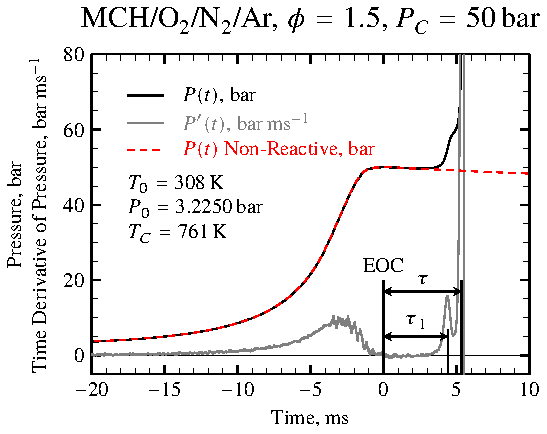
\includegraphics[width=12cm]{02-Experimental-Facilities/ign-delay-def}
    \caption{Representative pressure trace indicating the definition of
    the first stage and overall ignition delays and the corresponding
    non-reactive pressure trace. EOC stands for End of Compression.}
    \label{fig:ig-delay-def}
\end{figure}

Each unique $P_C$ and $T_C$ condition is repeated at least 5 times to
ensure repeatability of the experiments. The experiment closest to the
mean of the runs at a particular condition is chosen for analysis and
presentation. The standard deviation of all of the runs at a condition
is less than 10\% of the mean in all cases.

\subsection{Non-Reactive Experiments}

\Autoref{fig:ig-delay-def} also shows a non-reactive pressure trace.
Due to heat loss from the test mixture to the cold reactor walls,
the pressure and temperature of the gas in the reaction chamber will
decrease after the end of compression. A non-reactive pressure trace
is measured that corresponds to each unique $P_C$ and $T_C$ condition
studied to quantify the effect of the heat loss on the ignition process
and to verify that no heat release has occurred during the compression
stroke. The non-reactive pressure trace is acquired by replacing the
oxygen in the oxidizer with nitrogen, so that the specific heat ratio
of the initial mixture is maintained, but the heat release due to
exothermic oxidation reactions is eliminated. Maintaining a similar
specific heat ratio ensures that the non-reactive experiment faithfully
reproduces the conditions of the reactive experiment. A representative
non-reactive pressure trace is shown in \ref{fig:ig-delay-def}
corresponding to the experimental conditions in the figure.

\subsection{Reaction Chamber Homogeneity}

An RCM to be used for studies of homogeneous chemistry---as in this study---%
must ensure that homogeneous conditions exist inside the reaction
chamber for the duration of the experiment. Due to the high piston
velocities required to minimize heat loss and reaction during the
compression stroke, complex fluid mechanical effects can strongly
affect the state of the reactants at the EOC. The most important of these
effects is caused by the motion of the piston itself, where the piston
pushes the wall boundary layer into a roll-up vortex \cite{Lee1998}.
This cold vortex mixes with the hotter gases near the center of
the reaction chamber and causes large spatial inhomogeneities of
temperature and species.

To facilitate spatially homogeneous conditions in the reactor
and reduce the effect of the roll-up vortex, it is necessary to trap
the boundary layer. This is accomplished on the present RCM by a
crevice machined into the crown of the piston, shown in cross-section
in \autoref{fig:piston}. The boundary layer enters the crevice through
the converging section as the piston moves forward and is trapped
within the crevice. The dimensions of the crevice were optimized
by \textcite{Mittal2006a} through CFD simulations for high-pressure
conditions. Subsequently, \textcite{Mittal2006b} experimentally showed that
the optimized crevice design provides homogeneous conditions in the
reaction chamber up to approximately 150 milliseconds after the EOC.
By using PLIF measurements of acetone-seeded mixtures,
\textcite{Mittal2006b} showed that there was a core region of gases
near the center of the reactor whose temperature remained spatially
homogeneous.

\subsection{Determination of Reactant Temperature}

Two independent thermodynamic properties are required to fix the
thermodynamic state of the reactants in the reaction chamber at a
given time. The first property is the pressure, measured by the dynamic
pressure transducer, as discussed previously; the second property
is chosen to be the temperature.

In general, it is rather difficult to directly measure the temperature
of the gases in the reaction chamber during and after compression.
Intrusive methods such as thermocouples may introduce inhomogeneities into
the reaction chamber and non-intrusive optical techniques are difficult to set up
and require extensive calibration at the pressures of interest in RCM
studies. Thus, the temperature is determined indirectly by applying an
assumption called the "adiabatic core hypothesis" to the reaction chamber
\cite{Mittal2007, Lee1998}.

If all of the gases in the reaction chamber are compressed isentropically,
the temperature at the end of compression can be found by the
following relations:
%
\begin{subequations}
\label{eq:tic}
\begin{align}
\ln\left(\text{CR}\right) = \int_{T_0}^{T_{ic}} \! \frac{1}{T\left(\gamma-1\right)} \, \mathrm{d} T \\
\ln\left(\frac{P_{ic}}{P_0}\right) = \int_{T_0}^{T_{ic}} \! \frac{\gamma}{T\left(\gamma-1\right)} \, \mathrm{d} T
\end{align}
\end{subequations}
%
where CR is the volumetric compression ratio, $T_0$ is the initial temperature,
$T_{ic}$ is the temperature at the end of isentropic compression, $\gamma$ is the
temperature-dependent ratio of specific heats, $P_{ic}$ is the pressure at the
end of isentropic compression, and $P_0$ is the initial pressure.

However, experiments show that the measured pressure in the reaction chamber
does not reach the value of $P_{ic}$ calculated by using the geometric
compression ratio. The difference is due to finite heat loss from the
reactants to the reactor walls and the crevice volume during the
compression. Under the adiabatic core hypothesis, it is assumed that
the heat loss from the reactants only occurs in a thin boundary layer
near the wall, and the central core region is unaffected by heat loss
(i.e. the core is adiabatic) \cite{Desgroux1995}. Thus, the heat
loss is modeled as an effective reduction in the compression ratio, and
the temperature during the compression stroke can be calculated by:
%
\begin{align}
\ln\left(\frac{P_{C}}{P_0}\right) = \int_{T_0}^{T_{C}} \! \frac{\gamma}{T\left(\gamma-1\right)} \, \mathrm{d} T
\label{eq:tc}
\end{align}
%
where $P_C$ is the measured pressure at the end of compression, $T_C$
is the temperature at the end of compression, and the other variables
are the same as in \autoref{eq:tic}.

After the end of compression, the pressure in the reaction chamber
decreases, as can be seen in \autoref{fig:ig-delay-def}. This pressure
decrease is caused by heat loss from the reactants in the constant volume reaction
chamber and is accompanied by a decrease in the temperature of the
reactants. To model the thermodynamic state after the end of compression,
the adiabatic core hypothesis is applied, and the heat loss is
assumed to occur only in a thin boundary layer near the reactor walls.
Thus, the core region is modeled as adiabatic, and the heat loss
from the boundary layer can be modeled as an isentropic volume
expansion.

\subsection{Determination of Compressed Temperature}

In general, the specific heat ratio used in Eqs. (\ref{eq:tic}) and
(\ref{eq:tc}) is a function of temperature and composition, so \autoref{eq:tc} cannot
be integrated directly to find $T_C$. If the specific heats are parameterized with a
linear fit, it is possible to integrate \autoref{eq:tc} directly,
but this process is quite tedious; nonetheless, it will be applied in
\autoref{sec:uncertainty} to determine the uncertainty of $T_C$. In
general, the simplest method of calculating $T_C$ is to use software
numerically integrate \autoref{eq:tc}.

In this work, the CHEMKIN-Pro \cite{Chemkin2012} software is used to
perform the numerical integration and calculation of $T_C$. The
CHEMKIN-Pro software provides the facility for a user-specified
volume as a function of time to be applied to a homogeneous,
adiabatic reactor. Since the adiabatic core of the reaction chamber
is modeled as undergoing an isentropic volumetric compression followed
by an isentropic volumetric expansion, the user-specified volume
functionality is used to compute the RCM reactor state as a function
of time. A volume trace for simulation is computed from the measured
pressure trace using the isentropic relation:
%
\begin{align}
\frac{V_2}{V_1} = \left[\frac{P_1}{P_2}\right]^{\frac{1}{\gamma}}
\label{eq:volume-trace}
\end{align}
%
where $V_1$ and $V_2$ are the volumes at consecutive time points,
$P_1$ and $P_2$ are the pressures at consecutive time points, and
$\gamma$ is the temperature dependent specific heat. This equation
is applied during and after the compression stroke to calculate
the volume trace. In \autoref{eq:volume-trace} it is assumed that
changes in composition of the reactants are negligible during the
compression stroke.

For use in \autoref{eq:volume-trace}, $\gamma$ is tabulated for each
time point. Thus, the temperature at each time point must also be
computed by using the isentropic relation for temperature:
%
\begin{align}
\frac{T_2}{T_1} = \left[\frac{P_2}{P_1}\right]^{\frac{\gamma-1}{\gamma}}
\label{eq:isen-temp}
\end{align}
%
where $T_2$ and $T_1$ are the temperatures at consecutive time points.
Since $T_2$ depends on the value of $\gamma$, which in turn depends
on $T_2$, \autoref{eq:isen-temp} is iterated until the temperature
changes by less than one tenth of one percent on consecutive iterations.
Once again, it is assumed that changes in composition have a negligible
influence on the ratio of specific heats.
The temperature calculated by \autoref{eq:isen-temp} is typically within
1K of the temperature calculated by CHEMKIN-Pro.

\subsection{Uncertainty of Ignition Delay and Compressed Temperature}
\label{sec:uncertainty}
The uncertainty of the compressed temperature is an important paramter
to report. Since $T_C$ is not measured, we must perform an uncertainty
propagation analysis on the equation used to calculate $T_C$,
\autoref{eq:tc}. First, we simplify the term involving $\gamma$ in
\autoref{eq:tc}. By definition, $\gamma$ is the ratio of the specific heat
at constant pressure to that at constant volume
%
\begin{align}
\gamma = \frac{C_p}{C_v} = \frac{C_p/R}{C_v/R}
\end{align}

where $C_p$ and $C_v$ are the specific heats in molar units at constant
pressure and volume, respectively, and $R$ is the universal gas constant,
used to produce non-dimensional specific heats. Letting a hat denote the
non-dimensional specific heats, the difference between the non-dimensional
specific heats is one, $\hat{C}_v = \hat{C}_p - 1$. Then, it follows that
%
\begin{align}
\label{eq:simplify-gamma}
\frac{\gamma}{\gamma - 1} = \frac{\frac{\hat{C}_p}{\hat{C}_v}}{\frac{\hat{C}_p}{\hat{C}_v} - 1}
= \frac{\frac{\hat{C}_p}{\hat{C}_p - 1}}{\frac{\hat{C}_p}{\hat{C}_p - 1} - 1}
= \frac{\frac{\hat{C}_p}{\hat{C}_p - 1}}{\frac{1}{\hat{C}_p - 1}}
= \hat{C}_p
\end{align}

In \autoref{eq:tc}, the mean specific heat ratio for the mixture
should be used; thus, the simplification as shown in \autoref{eq:simplify-gamma}
requires that the specific heat $\hat{C}_p$ also be the mean specific
heat. In the following, we assume that there is negligible
change of the mean specific heat due to changes in reactant
mole fractions. The mean specific heat is simply the sum of the product of
the species mole fractions and their specific heats
%
\begin{subequations}
\label{eq:cp}
\begin{align}
C_{p\text{,total}} &= \sum_i X_i C_{p,i} \\
\hat{C}_{p\text{,total}} &= \frac{\sum_i X_i C_{p,i}}{R}
\end{align}
\end{subequations}
%
where $i$ indicates the species and $X_i$ is the species mole fraction.
In the NASA polynomial formulation used by CHEMKIN, the non-dimensional specific
heat at constant pressure as a function of temperature is represented by a
fourth-order polynomial fit
%
\begin{align}
\hat{C}_{p,i} = c_{1,i} + c_{2,i} T + c_{3,i} T^2 + c_{4,i} T^3 + c_{5,i} T^4
\end{align}
%
In general, this means that the specific heat can be non-linear. However,
the mixtures prepared in this study are composed primarily of
O$_2$, N$_2$ and Ar (i.e. no more than 5\% of any mixture is the
fuel), and the specific heats of O$_2$, N$_2$ and Ar are only weakly
temperature dependent over the range of temperatures experienced during
compression, we will approximate the total specific heat as a linear function
of temperature.
%
\begin{equation}%
\label{eq:cp-total}
\begin{split}
\hat{C}_{p\text{,total}} &= \sum_i X_i \hat{C}_{p,i} \\
&= \sum_i X_i \left( \sum_{j=1}^5 c_{j,i} T^{j-1} \right) \\
&\approx a + b T
\end{split}
\end{equation}
%
$a$ and $b$ are found by fitting the total non-dimensional specific heat
over the temperature range from 300--1100 K, as discussed below in
\autoref{sec:unc-cp}.

With this approximation of the specific heat, we can integrate \autoref{eq:tc}
to find the compressed temperature
%
\begin{subequations}
\begin{align}
\ln{\frac{P_C}{P_0}} &= \int_{T_0}^{T_{C}} \! \frac{\gamma}{T\left(\gamma-1\right)} \, \mathrm{d} T
                      = \int_{T_0}^{T_{C}} \! \frac{\hat{C}_p}{T} \, \mathrm{d} T \\
&= \int_{T_0}^{T_{C}} \! \frac{a + b T}{T} \, \mathrm{d} T\\
&= a \ln{T} + b T \Big|_{T_0}^{T_C}
\end{align}
\begin{equation}
\ln{\frac{P_C}{P_0}} = a \ln{T_C} + b \ln{T_C} - \left(a \ln{T_0} + b T_0\right) \label{eq:integrate-tc}
\end{equation}
\end{subequations}

Using a computer algebra system, \autoref{eq:integrate-tc} can be solved for $T_C$
%
\begin{align}
\label{eq:explicit-tc}
T_C = \frac{a W\!\!\left(\frac{b}{a} \exp\!{\left[\frac{b T_0}{a}\right]} T_0 \left[\frac{P_C}{P_0}\right]^{\frac{1}{a}}\right)}{b}
\end{align}
%
where $W(...)$ is Lambert's W function. With an explicit function for $T_C$, we can
estimate the uncertainty in $T_C$ by the root square sum of the uncertainty in the parameters in
\autoref{eq:explicit-tc}. The parameters are $P_C$, $P_0$, $T_0$, $a$, and $b$.
%
\begin{align}
\label{eq:tc-unc}
U_{T_C} = \sqrt{\left(\frac{\partial T_C}{\partial P_C} U_{P_C}\right)^2 + \left(\frac{\partial T_C}{\partial P_0} U_{P_0}\right)^2 +
                \left(\frac{\partial T_C}{\partial T_0} U_{T_0}\right)^2 + \left(\frac{\partial T_C}{\partial a} U_{a}\right)^2 +
                \left(\frac{\partial T_C}{\partial b} U_{b}\right)^2}
\end{align}

Once again using a computer algebra system, we find the partial derivatives of
\autoref{eq:explicit-tc} with respect to the parameters. Letting
%
\begin{equation*}
D = W\!\!\left(\frac{b}{a} \exp\!{\left[\frac{b T_0}{a}\right]} T_0 \left[\frac{P_C}{P_0}\right]^{\frac{1}{a}}\right)
\end{equation*}
%
the terms are
%
\begin{subequations}
\begin{align}
\frac{\partial T_C}{\partial P_C} &= \frac{D}{b P_C \left(D + 1\right)} \\
\frac{\partial T_C}{\partial P_0} &= \frac{-D}{b P_0 \left(D + 1\right)} \\
\frac{\partial T_C}{\partial T_0} &= \frac{\left(a + b T_0\right) D}{b T_0 \left(D + 1\right)} \\
\frac{\partial T_C}{\partial a} &= \frac{-D \left[b T_0 + \ln{\left(P_C/P_0\right)} - a D\right]}{a b \left(D + 1\right)} \\
\frac{\partial T_C}{\partial b} &= \frac{D\left(b T_0 - a D\right)}{{b}^2\left(D + 1\right)}
\end{align}
\end{subequations}

The uncertainties of the parameters, $U_j$ in \autoref{eq:tc-unc}, are in
general found by their own root square sum procedure.
%
\begin{align}
{U_j}^2 = {B_j}^2 + {R_j}^2
\end{align}
%
where the subscript $j$ represents one of the parameters in \autoref{eq:explicit-tc}.
The total uncertainty of a particular parameters is composed of
two parts, the systematic or bias uncertainty ($B_j$) and the
precision or random uncertainty ($R_j$). In general, the bias
uncertainty is contained in the measurement equipment and can
be reduced, e.g. by using different equipment; the random uncertainty
is inherent in any measured process and cannot be reduced by
experimental techniques. The bias and precision uncertainties
for each parameter will be discussed in the following.

\subsubsection{Uncertainty in Initial Temperature}

The bias uncertainty in the initial temperature is due to the standard
limits of error of the K-type thermocouple used to measure the
initial temperature. According to the Omega Engineering
specifications, this is "the greater
of $\SI{2.2}{\degreeCelsius}$ or 0.75\%". The largest initial temperatures
used in this work, 413 K, lead to an uncertainty of
$\pm \SI{3}{\kelvin}$; thus, $B_{T_O}=\SI{3}{K}$.
The precision uncertainty is due to the limit of precision of
the display on the Omega Engineering CNi3254 process meter used
to control the process temperature. This is $\pm\SI{0.5}{K}$.
The total uncertainty of the initial temperature is
%
\begin{align}
U_{T_0} = \sqrt{\left(B_{T_0}\right)^2 + \left(R_{T_0}\right)^2} = \sqrt{\left(\SI{3}{K}\right)^2 + \left(\SI{0.5}{K}\right)^2} = \SI{3.04}{K}
\end{align}

\subsubsection{Uncertainty in Initial Pressure}

The bias uncertainty in the initial pressure is due to the
standard error in the pressure transducer used to measure
the initial pressure. Two different pressure transducers have
been used in this study; the first, an Omega Engineering PX-303
(range: 0--50 psia), has a full scale uncertainty of 1.25\%, or
$\pm \SI{0.625}{psi} \ (\SI{4309.2}{Pa})$. The second transducer is an
Omega Engineering MMA100V10T2D0T4A6 type (range: 0--5200 torr) and was
purchased because preliminary results of this uncertainty analysis
indicated that the largest contributor to the uncertainty of $T_C$ was
the initial pressure measurement. The full scale uncertainty of the MMA
type transducers is 0.05\%, resulting in an uncertainty of
$\pm \SI{2.6}{torr} \ (\SI{346.6}{Pa})$, an order of magnitude lower than
the PX-303 while also providing more than double the operating range. Total
uncertainties using the appropriate pressure transducer are reported in
each experimental section of this work; both transducers will be analyzed
in this section.

The precision uncertainty is due to the limit of precision of the display
on the Omega Engineering DP41-B process meter used to monitor the initial
pressure. This is $\pm\SI{0.005}{torr} \ (\SI{0.666}{Pa})$. The total
uncertainty of the initial pressure is
%
\begin{subequations}
\begin{align}
U_{P_0} = \sqrt{\left(B_{P_0}\right)^2 + \left(R_{P_0}\right)^2} = \sqrt{\left(\SI{4309.2}{Pa}\right)^2 + \left(\SI{0.666}{Pa}\right)^2} = \SI{4309.2}{Pa} \\
U_{P_0} = \sqrt{\left(B_{P_0}\right)^2 + \left(R_{P_0}\right)^2} = \sqrt{\left(\SI{346.6}{Pa}\right)^2 + \left(\SI{0.666}{Pa}\right)^2} = \SI{346.6}{Pa}
\end{align}
\end{subequations}

\subsubsection{Uncertainty in Compressed Pressure}

The bias uncertainty in the compressed pressure is due to the standard
error in the piezoelectric pressure transducer. According to the
manufacturer calibration, the deviation of the full scale output from
linearity is less then 0.2\%, indicating that $B_{T_C}=\SI{0.5}{bar}$.
The uncertainties in the signal acquisition equipment are negligible
compared to this uncertainty. The precision uncertainty is due to the limit
of precision of the output of the pressure, and is 0.0000005 bar. This
is negligible compared to the bias uncertainty, so the total uncertainty
of the compressed pressure is
%
\begin{equation}
U_{P_C} = B_{T_C} = \SI{0.5}{bar}
\end{equation}

\subsubsection{Uncertainty in the Specific Heat}

\end{document}


%Butanol
% arara: xelatex: { synctex: on, shell: off }
% arara: biber
% arara: xelatex: { synctex: on, shell: off }
% arara: sumatrapdf
\documentclass[12pt, letterpaper]{article}

%Set the document font
\usepackage{fontspec}
\setmainfont[Renderer=Basic,Ligatures=TeX]{Times New Roman}

%Set the size of the margins and the paper
\usepackage[margin=1in, letterpaper]{geometry}

%Set the color of the links and PDF metadata
\usepackage[
    colorlinks=true,
    citecolor=blue,
    linkcolor=black
]{hyperref}

\hypersetup{%
    pdfinfo={
        Title={High Pressure Ignition Chemistry of Alternative Fuels},
        Author={Bryan W. Weber}
    }
}
%Set up the page numbers
%This has to go after geometry so the page number is centered
\usepackage{fancyhdr}
\pagestyle{fancy}
\fancyhf{}
\fancyfoot[C]{\thepage}
\renewcommand{\headrulewidth}{0pt}

%Set a command to easily skip a line
\newcommand{\blankline}{\vspace*{\baselineskip}}

%Set up biblatex
\usepackage[
    backend=biber,
    url=false,
    doi=true,
    sorting=none,
    sortcites=true,
    maxbibnames=6,
    minbibnames=6,
    maxcitenames=2,
    mincitenames=1,
    citestyle=numeric-comp,
    firstinits=true,
    isbn=false
]{biblatex}
\addbibresource{../library.bib}

%Remove the "In:" from before the journal title for articles
\renewbibmacro{in:}{%
  \ifentrytype{article}{}{\printtext{\bibstring{in}\intitlepunct}}}

%Set the sort order of the names in each bibliography entry
\DeclareNameAlias{default}{last-first}

%Don't print the article title. To print the title, add #1 to the last {}
\DeclareFieldFormat[article,incollection,unpublished]{title}{}

%Add Vol. and No. before volume and issue.
\DeclareFieldFormat[article]{volume}{\bibstring{volume}\addspace #1}
\DeclareFieldFormat[article]{number}{\bibstring{number}\addspace #1}

%Put a comma between the volume and issue instead of period
\renewbibmacro*{volume+number+eid}{%
  \printfield{volume}%
  \setunit{\addcomma\space}%<---- was \setunit*{\adddot}%
  \printfield{number}%
  \setunit{\addcomma\space}%
  \printfield{eid}}

%Add a comma after the journal title
\renewbibmacro*{journal+issuetitle}{%
  \usebibmacro{journal}%
  \setunit*{\addcomma\addspace}%
  \iffieldundef{series}
    {}
    {\newunit
     \printfield{series}%
     \setunit{\addspace}}%
  \usebibmacro{volume+number+eid}%
  \setunit{\addspace}%
  \usebibmacro{issue+date}%
  \setunit{\addcolon\space}%
  \usebibmacro{issue}%
  \newunit}

%Set the text to double spacing
\usepackage[doublespacing]{setspace}

%Packages not present in main.tex preamble
\usepackage{booktabs}

\def\chapterautorefname~#1\null{Chap.~#1\null}
\def\sectionautorefname~#1\null{Sec.~#1\null}
\def\subsectionautorefname~#1\null{Sec.~#1\null}
\def\figureautorefname~#1\null{Fig.~#1\null}
\def\tableautorefname~#1\null{Table~#1\null}
\def\equationautorefname~#1\null{Eq.~(#1)\null}

\newcommand{\Autoref}[1]{%
  \begingroup%
  \def\chapterautorefname~##1\null{Chapter~##1\null}%
  \def\sectionautorefname~##1\null{Section~##1\null}%
  \def\subsectionautorefname~##1\null{Sub--Section~##1\null}%
  \def\figureautorefname~##1\null{Figure~##1\null}%
  \def\tableautorefname~##1\null{Table~##1\null}%
  \def\equationautorefname~##1\null{Equation~##1\null}%
  \autoref{#1}%
  \endgroup%
}

\usepackage[font={footnotesize}]{caption}

\usepackage{mathtools}

\usepackage{multirow}

\graphicspath{ {../figures/} }

\newcommand{\linebreakcell}[2][c]{%
  \begin{tabular}[#1]{@{}c@{}}#2\end{tabular}}

%End of extra imports

\begin{document}
\section{Experimental Procedure}
\label{sec:buoh-proc}

The reactants used in this study, along with their purities, are shown in
\autoref{tab:buoh-expts}. To determine the relative proportions of each
reactant in the mixture, the absolute mass of fuel, the equivalence ratio
($\phi$), and the oxidizer ratio ($X_{O_2}:X_{\mathrm{inert}}$, where $X$
indicates mole fraction) are specified. \textit{s}- and \textit{i}-Butanol are
liquid at room temperature and have relatively low vapor pressure; therefore,
each is measured gravimetrically in a syringe to within 0.01 g of the specified
value. \textit{t}-Butanol is solid at room temperature (melting point: $25^{\circ}$ C),
and is melted before being handled in the same procedure as the other fuels.
The 17 L mixing tank is vacuumed to an ultimate pressure less than 5 Torr prior
to the injection of the liquid fuel through a septum. Proportions of O$_2$ and
N$_2$ are added manometrically at room temperature. The preheat temperature of
the RCM is set above the saturation point for each fuel to ensure complete
vaporization. A magnetic stirrer mixes the reactants. The temperature inside
the mixing tank is allowed to equilibrate for approximately 1.5 hours.

This approach to mixture preparation has been validated in several previous
studies by withdrawing gas samples from the mixing tank and analyzing the
contents by GC/MS \cite{Weber2011}, GC-FID \cite{Kumar2009}, and GC-TCD
\cite{Das2012}. These studies have verified the concentration of
\textit{n}-butanol, water, and \textit{n}-decane, respectively. In addition,
both the work by \textcite{Kumar2009} on \textit{n}-decane and the study of
\textcite{Weber2011} on \textit{n}-butanol confirmed that there was no fuel
decomposition over the course of a typical set of experiments. Furthermore,
within this study, each new mixture preparation is checked against previously
tested conditions to ensure reproducibility.

\Autoref{tab:buoh-expts} shows the experimental conditions considered in this
study. The compressed pressure conditions have been chosen to match the
previous \textit{n}-butanol study \cite{Weber2011}, but also to provide data in
regions not covered extensively in previous work. In addition, the fuel loading
conditions have been chosen to complement previous work; the studies by
\textcite{Stranic2012} and \textcite{Moss2008} used relatively dilute mixtures,
so we have included higher fuel loading conditions. Furthermore, the compressed
temperature conditions we have studied ($T_C=715$--$910$ K) have not been examined
in any other study, to our knowledge.

Each compressed pressure and temperature condition is repeated at least six
times to ensure repeatability. The mean and standard deviation of the ignition
delay for all runs at each condition are calculated. As an indication of
repeatability, the standard deviation is less than 10\% of the mean in every
case. Representative experimental pressure traces for simulations and
presentation are then chosen as the closest to the mean.

\begin{table}
    \centering
    \caption{Experimental Conditions and Reactant Purities}
    \label{tab:buoh-expts}
    \begin{tabular}{*{7}{c}}
    \toprule
    \multicolumn{5}{c}{Reactant (Purity)} & \multirow{3}[0]{*}{\linebreakcell{Equivalence \\ Ratio \\ $\phi$}} & \multirow{3}[0]{*}{\linebreakcell{Compressed \\ Pressure \\ $P_C$ (bar)}} \\
    \cmidrule{1-5}
    \linebreakcell{\textit{s}-butanol \\ (99.99\%)} & \linebreakcell{\textit{i}-butanol \\ (99.99\%)} & \linebreakcell{\textit{t}-butanol \\ (99.99\%)} & \linebreakcell{O$_2$ \\ (99.999\%)} & \linebreakcell{N$_2$ \\ (99.995\%)} & & \\
    \cmidrule{1-5}
    \multicolumn{5}{c}{Mole Percentage}   & & \\
    \midrule
    3.38  &       &       & 20.30 & 76.32 & 1.0   & 15 \\
    3.38  &       &       & 20.30 & 76.32 & 1.0   & 30 \\
          & 3.38  &       & 20.30 & 76.32 & 1.0   & 15 \\
          & 3.38  &       & 20.30 & 76.32 & 1.0   & 30 \\
          &       & 3.38  & 20.30 & 76.32 & 1.0   & 15 \\
          &       & 3.38  & 20.30 & 76.32 & 1.0   & 30 \\
          &       & 1.72  & 20.65 & 77.63 & 0.5   & 30 \\
          &       & 6.54  & 19.63 & 73.83 & 2.0   & 30 \\
    \bottomrule
    \end{tabular}
\end{table}

\section{Experimental Results}
\label{sec:buoh-expts}

\Autoref{fig:buoh-15bar} shows the ignition delays of the four isomers of
butanol measured in the RCM, at compressed pressure of $P_C=15$ bar for
stoichiometric mixture in air. The dashed line for each isomer is a least
squares fit to the data. The vertical error bars are two standard deviations
of the measurements of the ignition delay. The standard deviation is computed
based on all the runs at a particular compressed temperature and pressure
condition. A conservative estimate of the uncertainty in $T_C$ was calculated
in our previous work to be approximately 0.7–1.7\%. Due to the similar nature
of these experiments, and the similar properties of the fuels, this estimate
is considered to be valid for this study as well.

\Autoref{fig:buoh-15bar} demonstrates the differences in reactivity between
the isomers for stoichiometric fuel/air mixtures at compressed pressure
$P_C=15$ bar. \textit{n}-Butanol is clearly the most reactive, followed by
\textit{s}- and \textit{i}-butanol, which have very similar reactivities in
this temperature and pressure range. \textit{t}-Butanol is the least reactive.

The order of reactivity found in the RCM at 15 bar agrees with the shock tube
study at higher temperatures (approximately 1275−1667 K) and lower pressure
(1.5 atm) by \textcite{Stranic2012} but differs slightly from the studies of
\textcite{Moss2008} who measured ignition delays in a shock tube near 1.5 atm
and between 1275−1400 K, and \textcite{Veloo2011a} who measured
atmospheric-pressure laminar flame speeds. In particular, \textcite{Moss2008}
and \textcite{Veloo2011a} found distinct differences in reactivity between
\textit{s}- and \textit{i}-butanol, but the present study and the study by
\textcite{Stranic2012} found that they were nearly indistinguishable in terms
of reactivity under the conditions investigated. In addition,
\textcite{Stranic2012} noted some disagreement between their shock tube
ignition data and the data of \textcite{Moss2008} but their attempts to isolate
the cause could not discern what the difference might be caused by.

Further, the order of the reactivity of the butanol isomers also shows complex
temperature and pressure dependence. This is corroborated by the results shown
in \autoref{fig:buoh-30bar}. In \autoref{fig:buoh-30bar}, the order of
reactivity is different than in \autoref{fig:buoh-15bar}, where the only
variation between the plots is the compressed pressure; in
\autoref{fig:buoh-30bar} the compressed pressure is $P_C=30$ bar.
\autoref{fig:buoh-30bar} shows \textit{i}-butanol to be the least reactive,
\textit{s}-butanol to be less reactive than \textit{t}-butanol (but similar),
and \textit{n}-butanol to be the most reactive. Interestingly, the results of
the shock tube study by \textcite{Stranic2012} differ from those in the current
study at higher pressure (despite the agreement at lower pressure). In their
study, \textcite{Stranic2012} found \textit{i}- and \textit{n}-butanol to have
similar reactivity near 43 atm. in the temperature range of 1020--1280 K,
whereas in the present study we find \textit{i}-butanol to be the least
reactive of all four isomers at a pressure of 30 bar and over the temperature
range (715–910 K) investigated.

\begin{figure}
    \centering
    \begin{minipage}{7.9cm}
        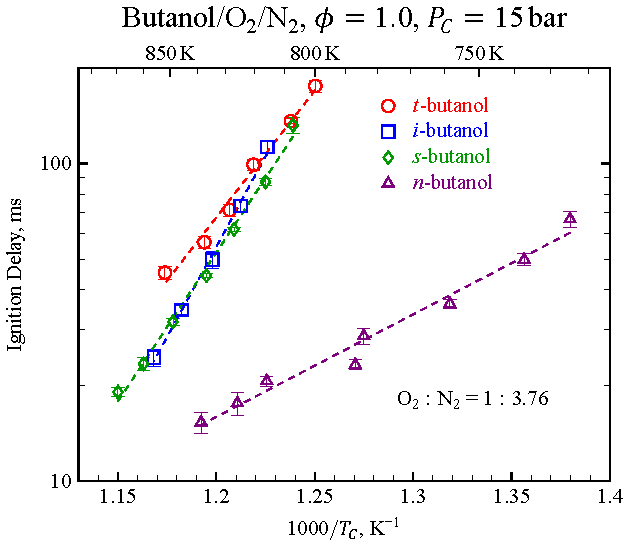
\includegraphics[width=7.9cm]{03-Butanol/buoh-15bar}
        \caption{Ignition delays of the four isomers of butanol at compressed
            pressure $P_C=15$ bar. Dashed lines are least squares fits to the
            data.}
        \label{fig:buoh-15bar}
    \end{minipage}
    \quad
    \begin{minipage}{7.9cm}
        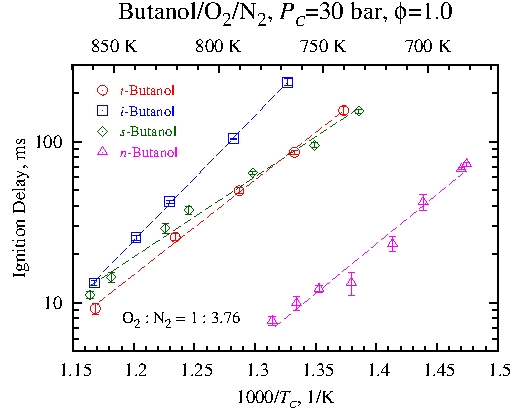
\includegraphics[width=7.9cm]{03-Butanol/buoh-30bar}
        \caption{Ignition delays of the four isomers of butanol at compressed
            pressure $P_C=30$ bar. Dashed lines are least squares fits to the
            data.}
        \label{fig:buoh-30bar}
    \end{minipage}
\end{figure}

The fact that \textit{t}-butanol becomes relatively more reactive than
\textit{i}- and \textit{s}-butanol as pressure increases is surprising at first
glance, and the reasons are not immediately apparent. Closer examination of the
pressure traces for each experiment gives one clue as to the cause of the
increased reactivity. \Autoref{fig:tbuoh-15bar} shows the pressure traces for
the \textit{t}-butanol experiments at 15 bar for stoichiometric mixtures in
air. It is evident that there is some pre-ignition heat release, because the
reactive pressure trace diverges from the non-reactive case prior to the
ignition event. Of the other isomers of butanol, only \textit{n}-butanol shows
any visible heat release prior to the main ignition event at 15 bar.

\Autoref{fig:tbuoh-phi10} shows the pressure traces for \textit{t}-butanol
experiments at 30 bar for stoichiometric mixtures in air. The effect of
pre-ignition heat release is even more striking in this figure, with
substantial changes in the slope of the pressure trace during the reactive
runs. Comparing to the pressure traces of the other isomers once again shows
that the magnitude of the pre-ignition heat release for \textit{t}-butanol is
much greater. Despite the appearance of early pressure rise, which is typically
indicative of two-stage ignition and low temperature chain branching, we do not
find a negative temperature coefficient region in terms of the ignition delay
response for any \textit{t}-butanol experiments. Therefore, we adopt the phrase
"pre-ignition heat release" rather than "two-stage ignition" in this work.

\begin{figure}
    \centering
    \begin{minipage}{7.9cm}
        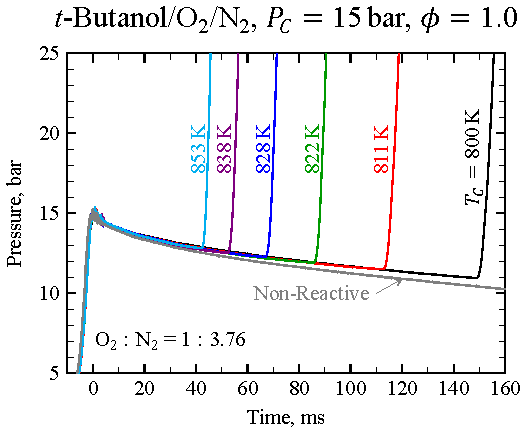
\includegraphics[width=7.9cm]{03-Butanol/tbuoh-15bar}
        \caption{Pressure traces of the 15 bar \textit{t}-butanol experiments,
            in stoichiometric air.}
        \label{fig:tbuoh-15bar}
    \end{minipage}
    \quad
    \begin{minipage}{7.9cm}
        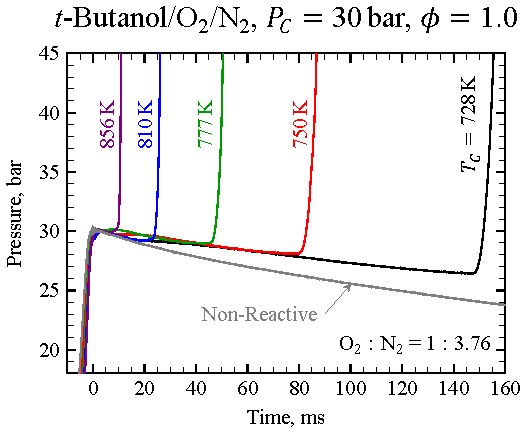
\includegraphics[width=7.9cm]{03-Butanol/tbuoh-phi10}
        \caption{Pressure traces of the 30 bar \textit{t}-butanol experiments,
            in stoichiometric air.}
        \label{fig:tbuoh-phi10}
    \end{minipage}
\end{figure}

In an effort to understand the reactions causing the pre-ignition heat release,
further experiments are conducted for \textit{t}-butanol at $P_C=30$ bar, for
equivalence ratios of 0.5 and 2.0 in air. \Autoref{fig:tbuoh-delays} shows
Arrhenius plots of the ignition delays for the three equivalence ratios. As
with the previous \textit{n}-butanol experiments at 15 bar \cite{Weber2011}
$\phi=0.5$ is the least reactive and $\phi=2.0$ is the most reactive. The
slopes are similar, indicating that the overall activation energies are similar
for the conditions investigated.

\begin{figure}
    \centering
    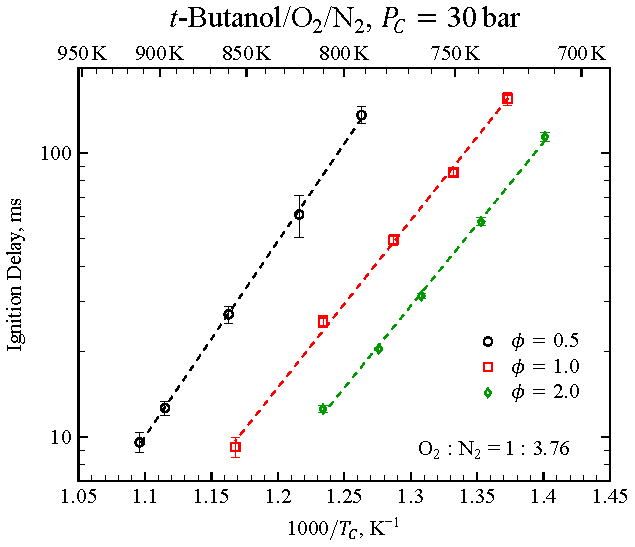
\includegraphics[width=12cm]{03-Butanol/tbuoh-delays}
    \caption{Ignition delays of three equivalence ratios of \textit{t}-butanol
    in air, for $P_C=30$ bar. Lines represent least squares fits to the data.}
    \label{fig:tbuoh-delays}
\end{figure}

A more interesting comparison is of the pressure traces of the three
equivalence ratios. It is clear from Figures \ref{fig:tbuoh-phi10},
\ref{fig:tbuoh-phi05}, and \ref{fig:tbuoh-phi20} that there are qualitative
differences in the pre-ignition heat release between the three equivalence
ratios. This is most likely due to the effect of the increased (reduced) fuel
mole fraction in the $\phi=2.0$ ($\phi=0.5$) case, since the mole fraction of
fuel is changed by +93\% (-49\%) compared to the $\phi=1.0$ case, while the
mole fraction of oxygen changes by only -3\% (+2\%) compared to the $\phi=1.0$
case, as shown in \Autoref{tab:buoh-expts}. Therefore, it appears that the
qualitative change in pre-ignition behavior is due to the change of fuel mole
fraction, where higher fuel loading promotes pre-ignition heat release.

\begin{figure}
    \centering
    \begin{minipage}{7.9cm}
        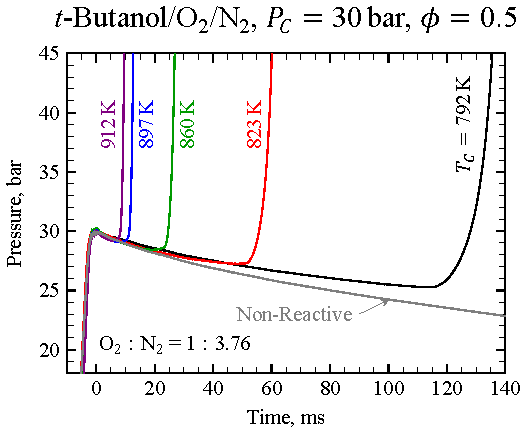
\includegraphics[width=7.9cm]{03-Butanol/tbuoh-phi05}
        \caption{Pressure traces of the 30 bar \textit{t}-butanol experiments,
            $\phi=0.5$ in air.}
        \label{fig:tbuoh-phi05}
    \end{minipage}
    \quad
    \begin{minipage}{7.9cm}
        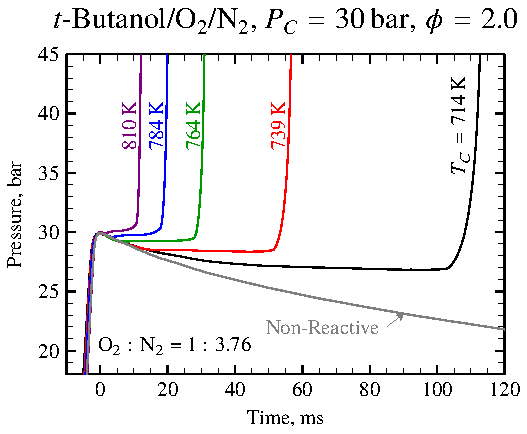
\includegraphics[width=7.9cm]{03-Butanol/tbuoh-phi20}
        \caption{Pressure traces of the 30 bar \textit{t}-butanol experiments,
            $\phi=2.0$ in air.}
        \label{fig:tbuoh-phi20}
    \end{minipage}
\end{figure}

\section{Simulation Results}
\label{sec:buoh-sims}

Simulations are performed with the kinetic mechanism from
\textcite{Sarathy2012} and a recent mechanism discussed in
\textcite{Hansen2013} and \textcite{Merchant2013} that is denoted as the MIT
mechanism hereafter. Other recent mechanisms, such as the mechanism from
\textcite{Frassoldati2012} do not include low temperature chemistry and are
therefore unable to reproduce the low-temperature ignition delays measured in
this study. The study by \textcite{Sarathy2012} validated their model for a
wide set of the existing experimental data. In terms of ignition delays, this
included the data from the study of \textcite{Stranic2012} up to 48 atm, our
previous study on \textit{n}-butanol \cite{Weber2011}, and the data being
published in this study at 15 bar. Importantly, the mechanism of
\textcite{Sarathy2012} was validated only for the 15 bar RCM data for all four
isomers, but not the 30 bar data also being published here. The MIT mechanism
\cite{Hansen2013,Merchant2013} was validated for \textit{i}-butanol
experiments, including pyrolysis and low pressure premixed flames; although the
model includes all four isomers of butanol as reactants, it has not been
optimized for any of the isomers except \textit{i}-butanol.

Figures \ref{fig:buoh-15sim} and \ref{fig:buoh-30sim} show comparison of the
VPRO simulations with the experimental data using the mechanism of
\textcite{Sarathy2012}. As \textcite{Sarathy2012} showed in their work (and as
we show here in \autoref{fig:buoh-15sim}), they found good agreement of the
model predictions with the present RCM data at 15 bar. At $P_C=30$ bar
(\autoref{fig:buoh-30sim}), similar degree of agreement is found for
\textit{t}-butanol and \textit{s}-butanol compared to $P_C=15$ bar, although
the \textit{s}-butanol results are under-predicted at high temperature and
over-predicted at low temperature. While the model of \textcite{Sarathy2012} is
able to well capture the overall activation energy of \textit{i}-butanol, it
under-predicts the experimental data by about a factor of 2–3. The
\textit{n}-butanol data are over-predicted by about a factor of 1.5.
Nevertheless, this agreement is quite good, especially considering that the
model is not validated for these conditions.

\begin{figure}
    \centering
    \begin{minipage}{7.9cm}
        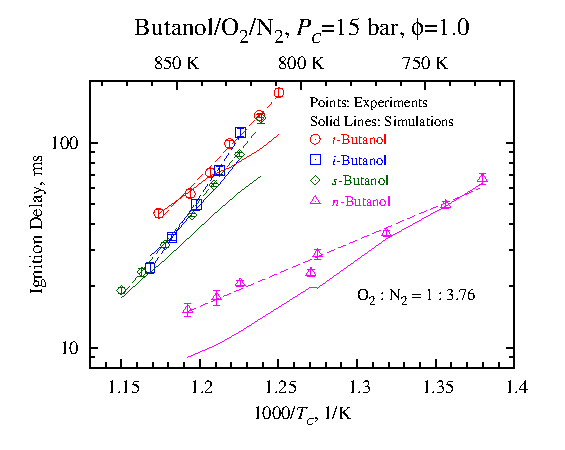
\includegraphics[width=7.9cm]{03-Butanol/buoh-15sim}
        \caption{$P_C=15$ bar, stoichiometric mixtures in air. Comparison of
            VPRO simulations using the kinetic mechanism of
            \textcite{Sarathy2012} with experimental ignition delays.}
        \label{fig:buoh-15sim}
    \end{minipage}
    \quad
    \begin{minipage}{7.9cm}
        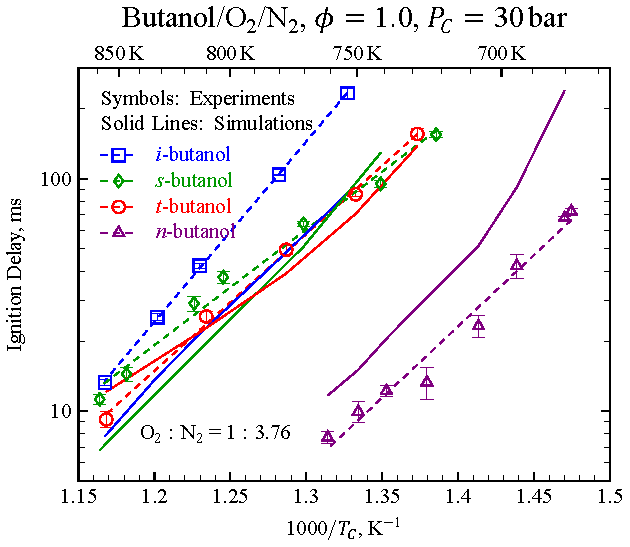
\includegraphics[width=7.9cm]{03-Butanol/buoh-30sim}
        \caption{$P_C=30$ bar, stoichiometric mixtures in air. Comparison of
            VPRO simulations using the kinetic mechanism of
            \textcite{Sarathy2012} with experimental ignition delays.}
        \label{fig:buoh-30sim}
    \end{minipage}
\end{figure}

VPRO simulations for \textit{n}- and \textit{s}-butanol (and also some
conditions for \textit{t}-butanol) using the MIT mechanism
\cite{Hansen2013,Merchant2013} do not ignite during the duration of the
simulations (the same as the experimental duration), and therefore no
simulations are shown for these fuels. In \autoref{fig:buoh-mit}, VPRO
simulations at 15 and 30 bar using both mechanisms are shown for
\textit{i}-butanol. It is seen that the mechanism from \textcite{Sarathy2012}
is in better agreement at 15 bar. However, at 30 bar the MIT mechanism
\cite{Hansen2013,Merchant2013} over-predicts the ignition delay (as at 15 bar),
while the \textcite{Sarathy2012} mechanism under-predicts the ignition delay.
The reason for these diverging predictions will be explored and discussed below.

\begin{figure}
    \centering
    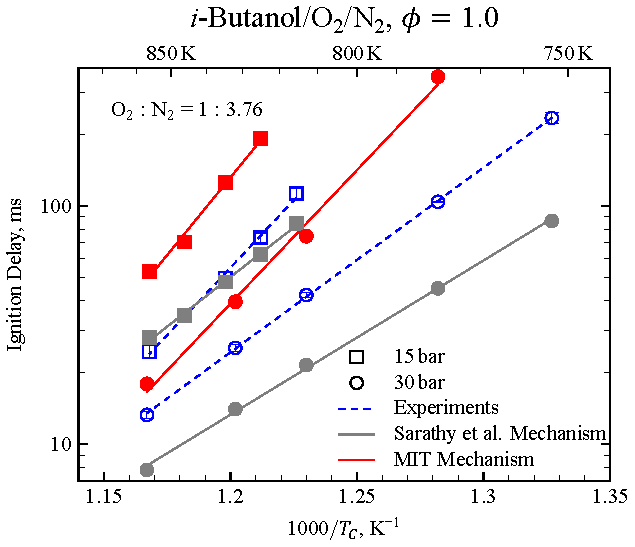
\includegraphics[width=12cm]{03-Butanol/buoh-mit}
    \caption{Comparison of VPRO simulations using the kinetic mechanism of
        \textcite{Sarathy2012} (solid lines) and the MIT mechanism
        \cite{Hansen2013,Merchant2013} (dotted lines) with the experimental
        ignition delay results (dashed lines) for stoichiometric mixtures of
        \textit{i}-butanol in air at $P_C=15$ bar (squares) and $P_C=30$ bar
        (circles).}
    \label{fig:buoh-mit}
\end{figure}

The agreement of the mechanism by \textcite{Sarathy2012} with the
off-stoichiometric mixtures of \textit{t}-butanol is also quite good, as shown
in \autoref{fig:tbuoh-sims}. Figures \ref{fig:tbuoh-05press}
-- \ref{fig:tbuoh-20press} show more detailed comparisons
of the simulated pressure traces and the experimental results, for similar
temperatures at the three equivalence ratios, respectively. Clearly, the
simulations also exhibit some pre-ignition heat release. In general, the
simulations qualitatively predict the pre-ignition heat release behavior at all
three equivalence ratios. The $\phi=0.5$ case has the least heat release and
the $\phi=2.0$ case has the most. Although the simulations are unable to match
the heat release behavior quantitatively, they match the experimental ignition
delays quite well. Considering the model is not validated for this temperature,
pressure, and equivalence ratio regime, the mismatch of the pre-ignition
behavior may not be of critical importance, depending on the application.

\begin{figure}
    \centering
    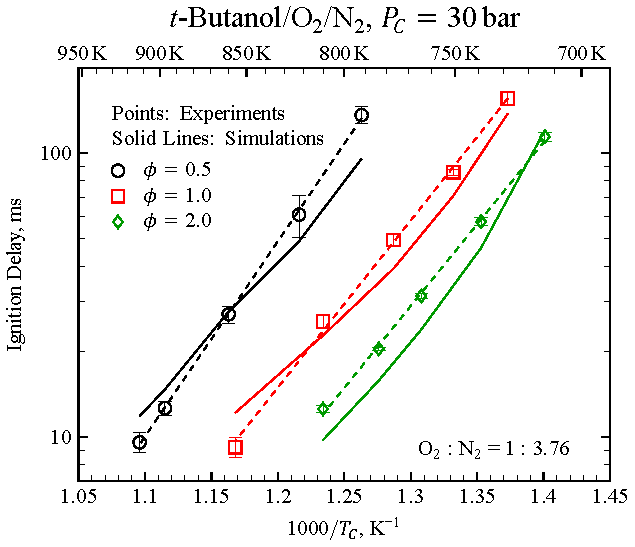
\includegraphics[width=12cm]{03-Butanol/tbuoh-sims}
    \caption{Comparison of the simulations using the kinetic mechanism of
        \textcite{Sarathy2012} for three equivalence ratio mixtures of
        \textit{t}-butanol in air at $P_C=30$ bar.}
    \label{fig:tbuoh-sims}
\end{figure}

\begin{figure}
    \centering
    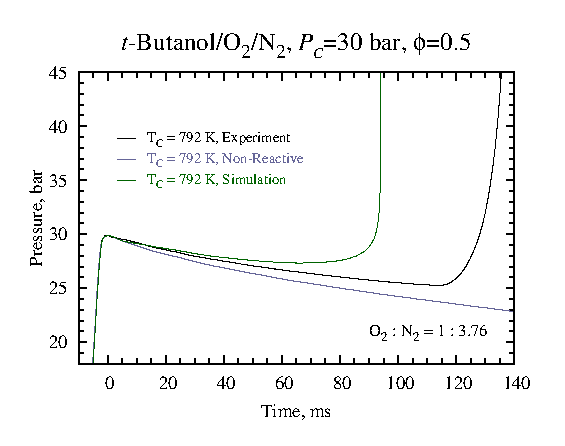
\includegraphics[width=12cm]{03-Butanol/tbuoh-05press}
    \caption{$\phi=0.5$ in air. Pressure traces of selected
        \textit{t}-butanol experiments compared with the corresponding
        non-reactive and simulated traces, using the mechanism of
        \textcite{Sarathy2012}.}
    \label{fig:tbuoh-05press}
\end{figure}

\begin{figure}
    \centering
    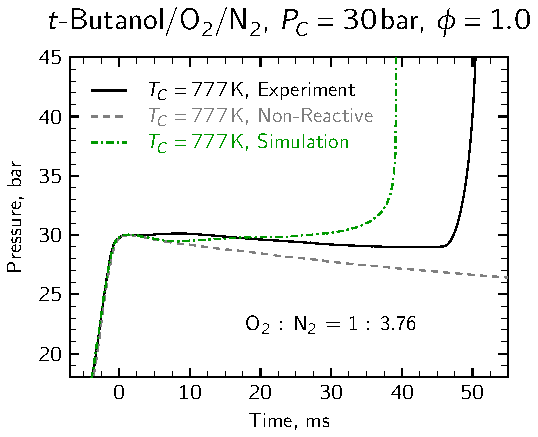
\includegraphics[width=12cm]{03-Butanol/tbuoh-10press}
    \caption{$\phi=1.0$ in air. Pressure traces of selected
        \textit{t}-butanol experiments compared with the corresponding
        non-reactive and simulated traces, using the mechanism of
        \textcite{Sarathy2012}.}
    \label{fig:tbuoh-10press}
\end{figure}

\begin{figure}
    \centering
    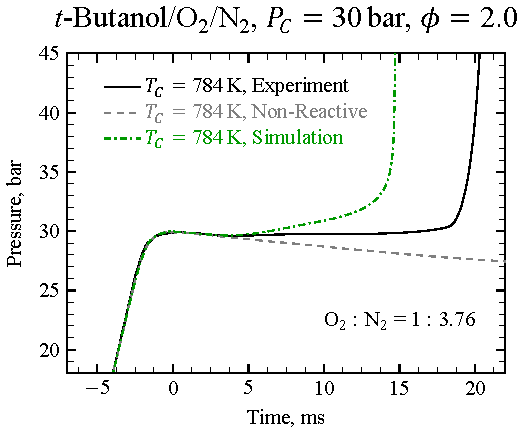
\includegraphics[width=12cm]{03-Butanol/tbuoh-20press}
    \caption{$\phi=2.0$ in air. Pressure traces of selected
        \textit{t}-butanol experiments compared with the corresponding
        non-reactive and simulated traces, using the mechanism of
        \textcite{Sarathy2012}.}
    \label{fig:tbuoh-20press}
\end{figure}

\section{Discussion}
\label{sec:buoh-discussion}

The relatively good agreement of the mechanism of \textcite{Sarathy2012} with
the experimental data, even for conditions at which the mechanism has not been
validated, suggests that using the mechanism to further interpret our
experimental data is not a facile exercise. In particular, Figures
\ref{fig:buoh-npath}--\ref{fig:buoh-ipath} show the initial steps of the fuel
breakdown process for each isomer. The percentages listed are the percent of
the reactant that is consumed to produce the product shown, by all the
reactions that can produce that product from the reactant (except where one
particular reaction is noted). These numbers are determined by integrating the
rate of production or consumption of each species by each reaction up to the
point of 20\% fuel consumption, and normalizing each reaction by the total
produced or consumed of each species up to that point. The 20\% fuel
consumption point is chosen because it is before small molecule chemistry takes
over to drive the ignition, and it has been used previously
\cite{Weber2011,Sarathy2012}. The rates of production are taken from a CONV
simulation, with initial conditions 750 K and 15 bar as well as 750 K and 30
bar. These conditions are representative of typical conditions after compression
in the present RCM experiments. The plain text percentages on top of the arrows
are the 15 bar case and the bold numbers underneath are for the 30 bar case.

In the following discussion, carbon-centered radicals are labeled according to
their distance from the hydroxyl moiety in the fuel molecule. Therefore, the
$\alpha$ carbon is the closest to the hydroxyl, followed by $\beta$, $\gamma$,
and $\delta$ carbons. Not all of the butanols have all of the types of carbons
listed here, due to varying chain lengths. For instance, \textit{t}-butanol has
one $\alpha$ carbon, three $\beta$ carbons, and no $\gamma$ or $\delta$ carbons.

As expected at the relatively low temperature of this analysis, H-abstraction
reactions dominate over unimolecular decomposition for all four isomers. It is
also expected that \textit{n}-, \textit{s}-, and \textit{i}-butanol react
primarily to their respective $\alpha$-hydroxybutyl radicals, since the
$\alpha$ C-H bond has the lowest energy \cite{Sarathy2012}. Due to its unique
structure, \textit{t}-butanol does not have an $\alpha$-hydroxybutyl radical
that can be formed by H-abstraction, so \textit{t}-butanol is primarily
consumed to form the $\beta$-hydroxybutyl radical, because the O-H bond energy
is much higher than $\beta$ C-H bond energies.

The unique structure of \textit{t}-butanol continues to affect the second level
of reactions as well. In the temperature and pressure regime investigated,
\textit{t}-butanol tends to add to molecular oxygen at the carbon radical site,
forming a hydroxybutylperoxy (RO$_2$) species. That this pathway is dominant is
due to the fact that \textit{t}-butanol has no $\alpha$-hydroxybutyl radical.
For the other three butanol isomers that do have an $\alpha$-hydroxybutyl
radical, the second level of reactions primarily produces an aldehyde + HO$_2$
by direct reaction –-- no hydroxybutylperoxy adduct is formed in this reaction,
and there is no possibility for typical hydrocarbon low-temperature chain
branching. Therefore, it is hypothesized that the pre-ignition heat release
seen in \textit{t}-butanol is caused by the oxygen addition to the fuel radical
to form $\beta$-hydroxybutylperoxy, which is an exothermic reaction.

\Autoref{fig:buoh-heat} shows the total cumulative heat release of each isomer
and the cumulative heat release of an important reaction for each of the
isomers (inset), from a CONV simulation with initial conditions of 750 K and 30
bar; analysis of 15 bar results is substantially similar. The cumulative heat
release in the inset is found by integrating the heat release by each reaction
with respect to time, while the reactions shown are the respective reactions
that have released the most heat up to the 20\% fuel consumption point for each
isomer. The abscissa of the plot is the fuel conversion, in percent. This
choice of x-axis allows a fair comparison of the heat release, because the
ignition delays of each isomer are markedly different, so comparing the heat
release with a time axis is more difficult. In \autoref{fig:buoh-heat},
exothermicity is represented by positive quantities.

In \autoref{fig:buoh-heat}, it is clear that \textit{t}-butanol has higher
heat release at low fuel consumption (during the induction period) than the
other three isomers. In addition, the primary heat release reaction for
\textit{t}-butanol has created much more heat than the primary reactions of the
other three isomers. As the reactions proceed, and the temperature increases,
the reverse reaction in the \textit{t}-butanol case becomes more important, and
the heat release contribution of this oxygen-addition reaction levels off. The
dominance of this reaction at early times is unique to \textit{t}-butanol
ignition, and appears to be driving the pre-ignition heat release.

\begin{figure}
    \centering
    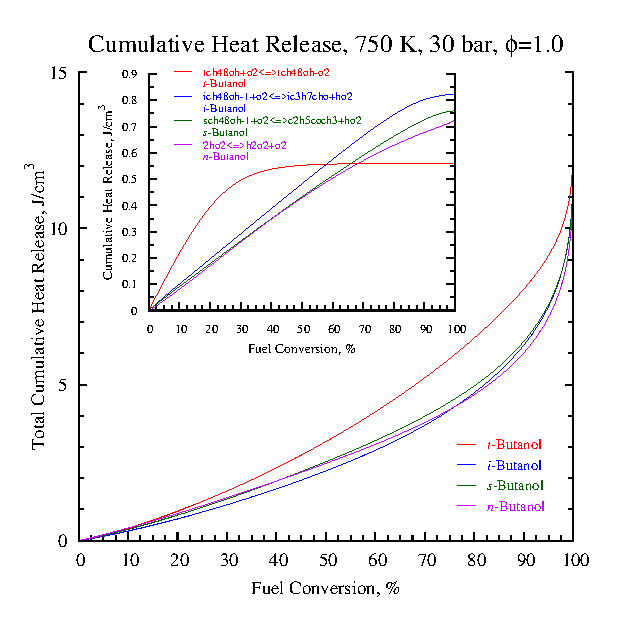
\includegraphics[width=10cm]{03-Butanol/buoh-heat}
    \caption{Total cumulative heat release and cumulative heat release by 
    important reactions (inset) as a function of fuel consumption from a 
    simulation using the mechanism of \textcite{Sarathy2012} with initial 
    conditions of 750 K and 30 bar, in stoichiometric air.}
    \label{fig:buoh-heat}
\end{figure}

Other researchers have also undertaken studies of the low to intermediate
temperature combustion of \textit{t}-butanol. \textcite{Lefkowitz2012}
performed a study in the Variable Pressure Flow Reactor (VPFR) at Princeton
University on the oxidation of \textit{t}-butanol over the temperature range
from 680−950 K, at 12.5 atm and stoichiometric mixture conditions. It is
interesting to note that they found no evidence of traditional hydrocarbon
low temperature chemistry. They did, however, find significant quantities of
acetone, peaking at approximately 800 K. \textcite{Lefkowitz2012} concluded
that the primary pathways of acetone formation are tautomerization of
propen-2-ol and $\beta$-scission of the alkoxy radical, based on an analysis
of the mechanism from \textcite{Grana2010}. Both of these pathways are
dependent on unimolecular decomposition of the hydroxybutyl radicals. However,
this mechanism has only been validated for flame studies; indeed, an updated
version of this model (by \textcite{Frassoldati2012}) is unable to predict the
low-temperature ignition delays measured in this study and hence is not
considered for analysis.

In contrast to the study of \textcite{Lefkowitz2012} path analysis of the
mechanism by \textcite{Sarathy2012} shows that unimolecular decomposition
of the hydroxybutyl radicals is not the most important pathway; as mentioned
earlier, the most important pathway is the formation of
$\beta$-hydroxybutylperoxy. Further analysis shows that the primary pathway of
reaction of the \textit{t}-butanol $\beta$-hydroxybutylperoxy species is
through the Waddington mechanism. The Waddington mechanism has been shown
experimentally to be an important pathway for $\beta$-hydroxypentylperoxy
radicals in the low temperature combustion of \textit{i}-pentanol
\cite{Welz2012}, as well as the $\beta$-hydroxybutylperoxy radicals of
\textit{i}- and \textit{t}-butanol \cite{Welz2013b}. \textit{t}-Butanol only
produces $\beta$-hydroxybutyl radicals, and one of the products of the
Waddington pathway in \textit{t}-butanol is acetone (the others are
formaldehyde and hydroxyl radical); over 88\% of the acetone produced up to the
20\% fuel consumption point is produced by the Waddington reaction. The study
in the VPFR thus provides further evidence of the importance of low-temperature
hydroxybutylperoxy chemistry in \textit{t}-butanol, although it is not
traditional hydrocarbon low-temperature chemistry.

Up to this point, the discussion has focused mainly on the importance of
hydroxybutylperoxy chemistry in \textit{t}-butanol. Nevertheless, the chemistry
of the hydroxybutylperoxy species is important in the combustion of the other
isomers of butanol as well. Using the high pressure shock tube at RWTH Aachen
University, \textcite{Vranckx2011} showed the importance of peroxy chemistry
pathways in the autoignition of \textit{n}-butanol. By adding a lumped peroxy
model to an existing kinetic model for \textit{n}-butanol combustion, they were
able to substantially improve agreement of the model with their experiments at
high pressure and low temperature. In their mechanism, \textcite{Sarathy2012}
included a semi-detailed peroxy chemistry model for all the isomers of butanol.
In fact, one of the main differences between the mechanism from
\textcite{Sarathy2012} and the MIT mechanism \cite{Hansen2013,Merchant2013} is
their respective treatment of the peroxy mechanism. Specifically,
oxygen-addition chemistry is not included in the MIT mechanism for
\textit{i}-butanol \cite{Hansen2013,Merchant2013}. In addition, the radical
that primarily controls \textit{i}-butanol decomposition is hydroxyl (OH) in
the mechanism of \textcite{Sarathy2012} (generated by the peroxy chemistry
sub-mechanism), but is hydroperoxyl (HO$_2$) in the MIT mechanism
\cite{Hansen2013,Merchant2013} (generated from the direct $\alpha$-hydroxybutyl
+ O$_2$=HO$_2$ + aldehyde formation pathway).

In their work, \textcite{Sarathy2012} used the reaction rates computed by
\textcite{DaSilva2009} for the hydroxyethyl system (i.e. ethanol as the parent
fuel) to determine the rate of direct reaction of $\alpha$-hydroxybutyl and
oxygen to form aldehyde and HO$_2$, and then set the rate of oxygen addition to
the $\alpha$-hydroxybutyl radical (to form $\alpha$-hydroxybutylperoxy) so that
the total rate was less than the collisional limit. The rates of oxygen
addition for the other radicals were prescribed depending on the type of carbon
(primary, secondary, or tertiary) based on studies of butane and
\textit{i}-octane \cite{Sarathy2012}. Based on the well-known importance of
hydroxyl in driving the reactivity of combustion systems, and the sources of
the estimates for the reaction rates of oxygen addition to hydroxybutyl (i.e.
the entry to the pathway that controls the rate of hydroxyl formation), it can
be hypothesized that the rates of hydroxybutylperoxy formation are
overestimated in the mechanism of \textcite{Sarathy2012}, as the simulated
results under-predict the experimental data of \textit{i}-butanol.

This hypothesis is supported by the results shown in \autoref{fig:buoh-sens},
which shows the linear brute force sensitivity of the ignition delay ($\tau$)
of \textit{i}-butanol to changes in the A-factor of the rate coefficient, using
the mechanism from \textcite{Sarathy2012}. The percent sensitivity is defined
as the difference between the ignition delay when the A-factor of each reaction
is halved and the nominal ignition delay, normalized by the nominal ignition
delay, as shown below:

\begin{equation}
    \label{eq:buoh-sens}
    S_i=\frac{\tau(0.5\mathrm{A}_i )-\tau(\mathrm{A}_i )}{\tau(\mathrm{A}_i)} \times 100\%
\end{equation}

Therefore, negative sensitivity means that halving the A-factor of a reaction
decreases the ignition delay, and positive sensitivity indicates the ignition
delay increases. These results are for CONV simulations with initial conditions
of 750 K and 30 bar as well as 1200 K and 30 bar.

The most sensitive reaction at the lower temperature is the initiation reaction
of the fuel with hydroperoxyl radical to form the primary fuel radical and the
second most sensitive reaction is the addition of oxygen to the primary
radical. Both of these reactions have positive sensitivities, indicating that
reducing the rate of these reactions would increase the ignition delay
(increasing the computed ignition delay will improve the agreement of the
simulations relative to the experiments in this case). It is apparent, then,
that reducing the amount of fuel propagating into the low temperature chain
branching pathway of oxygen addition to the primary $\alpha$-radical improves
the simulated results. Interestingly, the \textit{i}-butanol system is not
sensitive to the rates of oxygen addition to the hydroxybutyl radicals other
than the $\alpha$-radical. At the higher temperature of 1200 K, there is little
sensitivity on the ignition delay by changing the rate of the oxygen-addition
reaction, demonstrating its lack of influence at higher temperatures.

As a final comparison, we have modified this pathway in the mechanism from
\textcite{Sarathy2012} so that the rate of oxygen addition to the primary
fuel radical is arbitrarily set to zero; that is, the rate of the reaction
ic4h8oh-1+O2=ic4h8oh-1O2 is set to zero by zeroing the A-factor, while the
rates of the other oxygen addition reactions were unchanged. This unphysical
situation substantially changes the results of simulations for
\textit{i}-butanol --- removing this pathway in the mechanism from
\textcite{Sarathy2012} brings the simulations into close agreement with the
ignition delay results from the MIT mechanism \cite{Hansen2013,Merchant2013},
which does not consider this reaction for \textit{i}-butanol. Since the other
oxygen addition reactions were unchanged, it is apparent that the addition of
oxygen to $\alpha$-hydroxybutyl is one of the controlling reactions for the
high-pressure, low-temperature ignition of \textit{i}-butanol using the
mechanism of \textcite{Sarathy2012}. It is therefore concluded that a detailed
examination of the rates of direct formation of aldehyde+HO$_2$ and oxygen
addition to the $\alpha$-hydroxybutyl radical are required to better predict
the low-temperature ignition behavior of \textit{i}-butanol. Furthermore, based
on the other results of this study, a detailed analysis of the oxygen addition
reactions to all the isomers of butanol is probably warranted.

\section{Conclusions}
\label{sec:buoh-conclusions}

In this work, ignition delays for all four isomers of butanol in stoichiometric
mixture with air have been presented over the low to intermediate temperature
range, and at two compressed pressures of 15 and 30 bar. The order of
reactivity of the isomers goes \textit{n}-butanol$>$\textit{s}-butanol$\approx$
\textit{i}-butanol$>$\textit{t}-butanol at the lower pressure, but changes to
\textit{n}-butanol$>$\textit{t}-butanol$>$\textit{s}-butanol$>$
\textit{i}-butanol at the higher pressure. This unexpected result is partially
explained by the fact that there is substantial pre-ignition heat release
present for \textit{t}-butanol. To help understand the nature of the
pre-ignition heat release of \textit{t}-butanol, studies at off-stoichiometric
conditions, $\phi=0.5$ and $\phi=2.0$ in air, are also conducted.

Comparisons of the experimentally measured ignition delays with two kinetic
mechanisms show good agreement for certain isomers, but relatively poorer
agreement for others. The kinetic mechanism of \textcite{Sarathy2012} is used
to further elucidate the chemical processes controlling the autoignition of
these butanol isomers. Pathway analysis of the fuel decomposition shows that
\textit{n}-, \textit{s}-, and \textit{i}-butanol primarily form
$\alpha$-hydroxybutyl radicals, because the proximity of the $\alpha$ carbon to
the hydroxyl group reduces the C-H bond energy. The α-hydroxybutyl radicals
tend to form an aldehyde plus HO$_2$  directly, without forming a
hydroxybutylperoxy complex. However, due to its unique structure,
\textit{t}-butanol can only form $\beta$-radicals; these radicals do not have
the tendency to react with oxygen to directly form HO$_2$  and an aldehyde.
Rather, \textit{t}-butanol preferentially adds oxygen to the fuel radical site.
It is hypothesized that this reaction, O$_2$  addition to form
hydroxybutylperoxy, causes the pre-ignition heat release in \textit{t}-butanol
and leads to a chain propagation pathway through the Waddington mechanism. The
fact that this oxygen-addition reaction is preferred is unique to
\textit{t}-butanol, although a detailed understanding of the peroxy chemistry
of alcohols is still of vital importance to the other butanol isomers. This is
further demonstrated in this work for the case of \textit{i}-butanol, where the
ignition delay is shown to be quite sensitive to both the rate of primary fuel
radical formation and to the rate of oxygen addition to the primary fuel
radical. It is also noted that \textit{n}-butanol autoignition was shown to be
quite sensitive to peroxy chemistry in the study of \textcite{Vranckx2011}.

All together, these analyses show the importance of the peroxy chemistry
pathways in the autoignition of the butanols. Further experimental studies,
such as species profiles from the low temperature ignition of the butanol
isomers, could help reduce uncertainty in the pathways of fuel breakdown.
Finally, further understanding of the rates of the peroxy pathways is
important and therefore further theoretical and quantum chemical studies are
warranted.

\end{document}


%iso-Pentanol
% arara: lualatex: { synctex: on, shell: off }
% arara: biber
% arara: lualatex: { synctex: on, shell: off }
% arara: sumatrapdf
\documentclass[../main.tex]{subfiles}

\begin{document}

\begin{figure}[!ht]\CenterFloatBoxes
    \begin{floatrow}
        \killfloatstyle\ttabbox
        {\captionsetup{type=table}\caption{HHV of Ethanol, \textit{i}-Pentanol, and Gasoline}
        \label{tab:ipeoh-heats}}
        {\begin{tabular}{*{4}{c}}
            \toprule
            Compound & Ethanol \cite{Afeefy2014} & \textit{i}-Pentanol \cite{Afeefy2014} & Gasoline \cite{Davis2013} \\
            \midrule
            HHV [\si[per-mode=symbol]{\mega\joule\per\kilo\gram}] & 29.67 & 37.73 & 48.46 \\
            \bottomrule
        \end{tabular}}
        \ffigbox[\FBwidth]
            {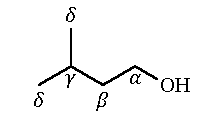
\includegraphics[width=5cm]{04-Pentanol/ipeoh-skeletal}}
            {\caption{Skeletal structure of \iPeOH{}}
            \label{fig:ipeoh-skeletal}}
    \end{floatrow}
\end{figure}

\section{Structure of \textit{i}-Pentanol}
\label{sec:ipeoh-struct}

\textit{i}-Pentanol (3-methyl-1-butanol) is a five-carbon alcohol whose
skeletal structure is shown in \cref{fig:ipeoh-skeletal}. The carbon
atoms in \cref{fig:ipeoh-skeletal} are labeled according to their
distance from the hydroxyl moeity, with $\alpha$ being the closest and
$\delta$ being the farthest. The Greek letter notation will be used to
refer to the carbon-centered radicals in \cref{sec:ipeoh-discussion}.
\textit{i}-Pentanol can be produced biologically \cite{Peralta-Yahya2012},
and offers several similar advantages as the butanol isomers compared
to ethanol. \Cref{tab:ipeoh-heats} compares the HHV of ethanol, \iPeOH{},
and gasoline.

\section{Experimental Procedure}
\label{sec:ipeoh-procedure}

Experiments for \iPeOH{} in the RCM have been performed at the conditions listed
in \cref{tab:ipeoh-expts}. Homogeneous fuel and air pre-mixtures are prepared in a
\SI{17.56}{\liter} mixing tank. The mixing tank and all tubes and manifolds
connecting the tank with the RCM are heated, allowing the study of
relatively low vapor pressure fuels. The initial temperature is set above
the saturation temperature of \iPeOH{} for each mixture studied. Initial
temperatures in the range \SIrange{353}{413}{\kelvin} were used in this
study. The mixing tank is equipped with a magnetic stirrer to ensure homogeneity
of the mixture.

\begin{table}
    \caption{\iPeOH{} Experimental Conditions}
    \label{tab:ipeoh-expts}
    \begin{tabular}{*{5}{c}}
    \toprule
    \multicolumn{3}{c}{Reactant (Purity)} & \multirow{3}[0]{*}{\linebreakcell{Equivalence \\ Ratio \\ $\phi$}} & \multirow{3}[0]{*}{\linebreakcell{Compressed \\ Pressure \\ $P_C$ (bar)}} \\
    \cmidrule{1-3}
    \linebreakcell{\iPeOH{} \\ (\SI{99.6}{\percent})} & \linebreakcell{\ce{O2} \\ (\SI{99.994}{\percent})} & \linebreakcell{\ce{N2} \\ (\SI{99.999}{\percent})} & & \\
    \cmidrule{1-3}
    \multicolumn{3}{c}{Mole Percentage}   & & \\
    \midrule
    2.41 & 20.50 & 77.09 & 1.0 & 40 \\
    1.22 & 20.75 & 78.03 & 0.5 & 40 \\
    4.71 & 20.01 & 75.27 & 2.0 & 40 \\
    \bottomrule
    \end{tabular}
\end{table}

Prior to mixture preparation, the mixing tank is vacuumed to less than
\SI{1}{\torr}, whereupon liquid fuel (\iPeOH{}, Sigma-Aldrich, \SI{99.6}{\percent}
purity) is injected by a syringe through a septum. The syringe is massed
before and after the injection, with the difference being the amount of
fuel in the mixing tank. Based on this mass, required proportions of
the gaseous oxidizer (\ce{O2}, \SI{99.994}{\percent} purity, \ce{N2}, \SI{99.999}{\percent} purity) are
calculated. The gases are added to the mixing tank sequentially at
room temperature and the total pressure is monitored to ensure that the
proper mixture concentrations are attained. Finally, the heaters and
stirring vane are switched on and the system is allowed approximately
\SI{1.5}{\hour} to reach steady state.

\section{Model Improvements}
Through collaboration with researchers at Lawrence Livermore National
Laboratory, many improvements to the chemical kinetic model for \iPeOH{} were
made relative to the work of \textcite{Tsujimura2012}. Some of the major
improvements are highlighted below; see the article for more detail
\cite{Sarathy2013}.

\begin{enumerate}
\item The model was restructured based on work with \ce{C4} and \ce{C5}
      alcohols \cite{Sarathy2012, Heufer2012a}
\item The most stable conformers of \iPeOH{} were calculated using
      quantum chemistry software
\item The bond dissociation energies (BDEs) of the of the C-C, C-H, C-O, and O-H bonds were calculated
      using quantum chemistry software
\item The model includes the Waddington pathway shown to be important in
      low-temperature decomposition of \iPeOH{} by \textcite{Welz2012}
\item New reaction pathways were added based on the work of \textcite{Welz2012,
      Welz2013}, including the unconventional water-elimination pathway discussed
      in \textcite{Welz2013}
\end{enumerate}

Moreover, the following data sets from the literature and presented in
the work of \textcite{Sarathy2013} were used to validate the newly
updated model, in addition to the new data at $P_C=\SI{40}{\bar}$ presented here.

\begin{enumerate}
\item Ignition delays measured in a ST and an RCM \cite{Tang2013, Tsujimura2012}
\item JSR species data \cite{Dayma2011}
\item New ignition delays measured in STs \cite{Sarathy2013}
\item New JSR species data \cite{Sarathy2013}
\item New flame speed and flame extinction measurements \cite{Sarathy2013}
\end{enumerate}

\section{Experimental \& Modeling Results}
\label{sec:ipeoh-results}

The experimental ignition delays measured in the RCM are shown in
\cref{fig:ipeoh-7bar,fig:ipeoh-20bar,,fig:ipeoh-40bar}, along with
ignition delays measured in the ST and comparison with
the model simulations. There is no $\phi=2.0$ data set for \SI{7}{\atmosphere}
because no conditions at which ignition occurred could be found.
In \cref{fig:ipeoh-7bar,fig:ipeoh-20bar,fig:ipeoh-40bar}, solid
lines represent adiabatic, constant volume simulations, and dashed
lines represent volume-profile simulations.

\begin{figure}
    \ffigbox[\FBwidth]
        {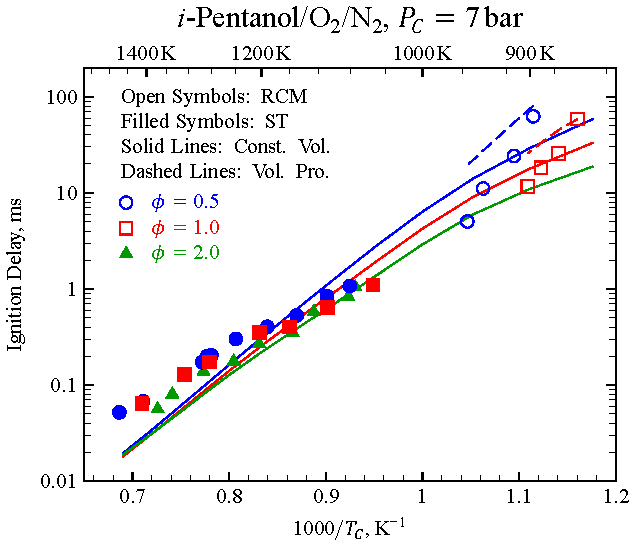
\includegraphics[width=10cm]{04-Pentanol/ipeoh-7bar}}
        {\caption{ST and RCM ignition delay times published in
        \textcite{Tsujimura2012} at \SI{7}{\atmosphere} compared
        with model predictions by the model from \textcite{Sarathy2013}.
        The RCM studies were conducted as part of this thesis.}
        \label{fig:ipeoh-7bar}}
    \par
    \vspace{10pt}
    \ffigbox[\FBwidth]
        {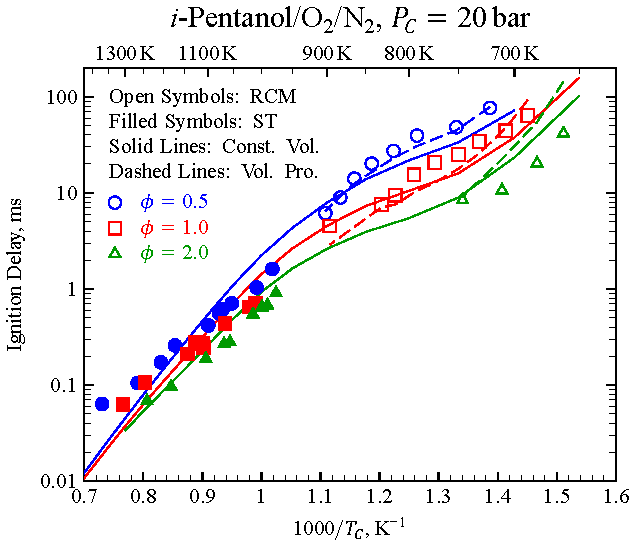
\includegraphics[width=10cm]{04-Pentanol/ipeoh-20bar}}
        {\caption{ST and RCM ignition delay times published in
        \textcite{Tsujimura2012} at \SI{20}{\atmosphere} compared
        with model predictions by the model from \textcite{Sarathy2013}.
        The RCM studies were conducted as part of this thesis.}
        \label{fig:ipeoh-20bar}}
\end{figure}
\begin{figure}
    \ffigbox[\FBwidth]
        {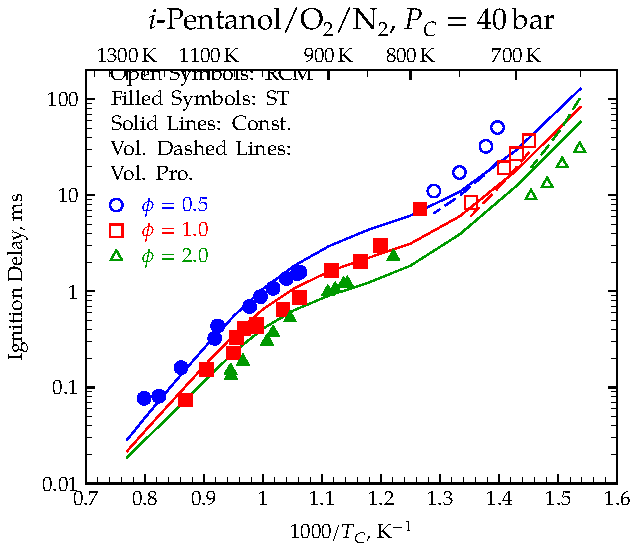
\includegraphics[width=10cm]{04-Pentanol/ipeoh-40bar}}
        {\caption{ST and RCM ignition delay times published in
        \textcite{Sarathy2013} at \SI{40}{\atmosphere} compared
        with model predictions by the model from \textcite{Sarathy2013}.
        The RCM studies were conducted as part of this thesis.}
        \label{fig:ipeoh-40bar}}
    \par
    \vspace{10pt}
    \ffigbox[\FBwidth]
        {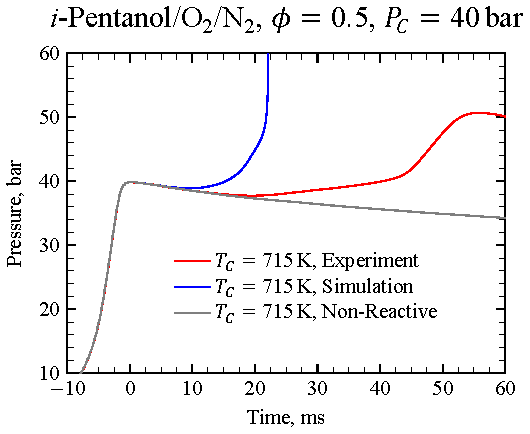
\includegraphics[width=10cm]{04-Pentanol/ipeoh-phi05}}
        {\caption{Experimental reactive (red, solid), simulated reactive
        (blue, dashed), and experimental non-reactive (gray, dot-dashed) pressure
        profiles at \SI{40}{\atmosphere} for lean \iPeOH{}/air mixtures.}
        \label{fig:ipeoh-phi05}}
\end{figure}
\begin{figure}
    \ffigbox[\FBwidth]
        {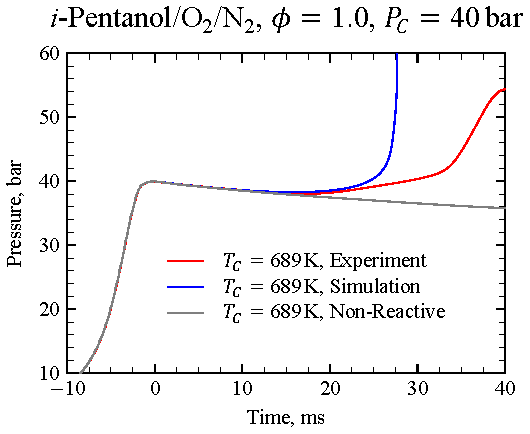
\includegraphics[width=10cm]{04-Pentanol/ipeoh-phi10}}
        {\caption{Experimental reactive (red, solid), simulated reactive
        (blue, dashed), and experimental non-reactive (gray, dot-dashed) pressure
        profiles at \SI{40}{\atmosphere} for stoichiometric \iPeOH{}/air mixtures.}
        \label{fig:ipeoh-phi10}}
    \par
    \vspace{10pt}
    \ffigbox[\FBwidth]
        {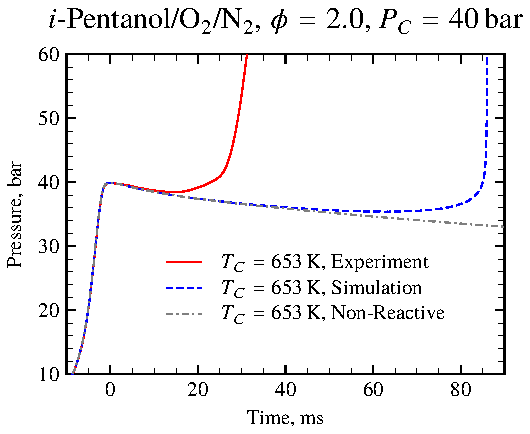
\includegraphics[width=10cm]{04-Pentanol/ipeoh-phi20}}
        {\caption{Experimental reactive (red, solid), simulated reactive
        (blue, dashed), and experimental non-reactive (gray, dot-dashed) pressure
        profiles at \SI{40}{\atmosphere} for rich \iPeOH{}/air mixtures.}
        \label{fig:ipeoh-phi20}}
\end{figure}

At \SI{7}{\atmosphere} (\cref{fig:ipeoh-7bar}), the high-temperature ignition delays
measured in the ST are generally predicted to within a factor of 1.5. The RCM experiments
are also well predicted at low temperature---within a factor of 2---but
the disagreement grows to approximately a factor of 4 in the
intermediate temperature regime. At \SI{20}{\atmosphere} (\cref{fig:ipeoh-20bar}), the
high-temperature ignition delays are well predicted, including
capturing the equivalence ratio sensitivity of the ignition delays.
The ignition delays measured in the RCM are fairly well predicted
at the lean and stoichiometric conditions, but are over-predicted
at the rich condition.

At \SI{40}{\atmosphere} (\cref{fig:ipeoh-40bar}), the model is able to
reproduce the high-temperature ignition delays fairly well, including
capturing the equivalence ratio dependence of the ignition delays.
Ignition delay data near \SI{40}{\atmosphere} and temperatures
ranging from \SIrange{651}{776}{\kelvin} were also acquired using the
RCM. The ignition data in the RCM and ST are in good qualitative
agreement, displaying the expected decrease in ignition delay with
increasing temperature. The model well predicts the observed trend
of decreasing ignition delay time with increasing equivalence
ratio, which occurs because a higher fuel concentration results
in greater radical production at these conditions. Constant volume
and volume history simulations at the \SI{40}{\atmosphere} RCM
conditions (\cref{fig:ipeoh-40bar}) indicate the model can well predict
ignition delay times at stoichiometric conditions, but cannot well predict
RCM ignition delay data at lean and rich conditions. The difference
(i.e.\ spread) in ignition delay times across various equivalence ratios
is similar to that observed for other alcohols in the same facilities
(e.g.\ \nBuOH{} at \SI{15}{\bar} \cite{Weber2011} and \tBuOH{} at
\SI{30}{\bar} \cite{Weber2013}). The primary issue with the model is
its equivalence ratio sensitivity; predicted ignition delay times need
to be increased at lean conditions yet decreased at rich conditions,
implying that the system's reactivity is controlled by different phenomenon
at different equivalence ratios. At these low temperatures the model's
reactivity is driven by the overall peroxy reaction sequence,
R+\ce{O2}=ROO=QOOH+\ce{O2}=OOQOOH=2OH+products, including the inhibitive
direct (i.e., concerted) \ce{HO2} elimination and QOOH decomposition routes.
An increase (or decrease) in any reaction rate constant along this
reaction sequence will move the reactivity of the system in the same
direction at all equivalence ratios. Therefore, we were unable to
identify a single reaction rate constant modification that would decrease
overall reactivity at lean conditions while increase it at rich conditions.

Representative experimental and simulated pressure profiles for the lean,
stoichiometric, and rich conditions are shown in
\cref{fig:ipeoh-phi05,fig:ipeoh-phi10,,fig:ipeoh-phi20} respectively,
with the profiles shifted so EOC occurs at \SI{0}{\second}. Interestingly,
the experimental pressure traces after the induction period do not show
a sharp increase in pressure (i.e., heat release is more gradual,
similar to two-stage ignition). For the lean case, there is a moderate
heat release \SI{25}{\milli\second} after EOC followed by a larger heat
release event, and similar behavior is observed at other equivalence ratios.
It is noted that similar heat release prior to the main ignition event
was found in an HCCI engine experiment using \iPeOH{} by \textcite{Yang2010}
and was termed Intermediate Temperature Heat Release (ITHR) in their
work.

The pressure profile of the present simulations qualitatively
agrees with the experimental data, in that the simulated pressure
traces deviate from the non-reactive trace prior to the main ignition
event, although the ignition delay itself does not necessarily
agree very well. For lean and stoichiometric cases the simulated
ignition delay times are fast compared to the data, whereas at rich
conditions they are too slow.

\section{Discussion}
\label{sec:ipeoh-discussion}

The sensitivity of the ignition delay to changes in the reaction rate
coefficients is shown in \cref{fig:ipeoh-20sens} for a constant volume,
adiabatic simulation at \SI{20}{\atmosphere}, \SI{800}{\kelvin}, and for
equivalence ratios varying from $\phi=\numrange{0.5}{2.0}$. The percent
sensitivity is computed by the formula:
%
\begin{align}
S = \frac{\tau(2k_i)-\tau(k_i)}{\tau(k_i)} \times \SI{100}{\percent}
\end{align}
%
where $\tau(2k_i)$ is the ignition delay when the rate coefficient of
reaction $i$ is doubled, and $\tau(k_i)$ is the nominal ignition delay.
Positive sensitivities therefore represent an increase in the ignition
delay when the rate coefficient of reaction $i$ is increased. Both the
forward and reverse rates of each reaction are increased simultaneously.
Since the reaction 2ho2$\Leftrightarrow$h2o2+o2 is represented by two sets of $\mathrm{A}$, $b$,
and $E_a$ in the reaction mechanism, both Arrhenius coefficients were
simultaneously doubled to give the sensitivity value shown in \cref{fig:ipeoh-20sens}.

\begin{figure}
    \ffigbox
        {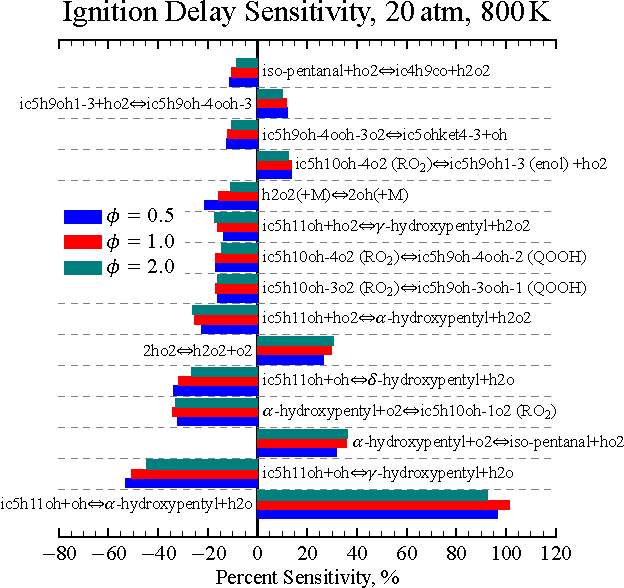
\includegraphics[width=10cm]{04-Pentanol/ipeoh-20sens}}
        {\caption{Sensitivity of the ignition delay to changes in
        the reaction rate coefficients for three equivalence ratios.
        Initial conditions for constant-volume adiabatic simulations are
        \SI{800}{\kelvin} and \SI{20}{\atmosphere}.}
        \label{fig:ipeoh-20sens}}
    \par
    \vspace{10pt}
    \ffigbox
        {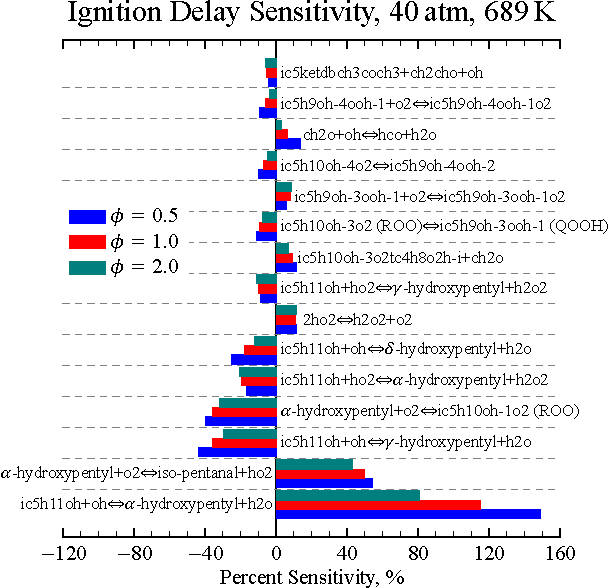
\includegraphics[width=10cm]{04-Pentanol/ipeoh-40sens}}
        {\caption{Sensitivity of the ignition delay to changes in
        the reaction rate coefficients for three equivalence ratios.
        Initial conditions for constant-volume adiabatic simulations are
        \SI{689}{\kelvin} and \SI{40}{\atmosphere}.}
        \label{fig:ipeoh-40sens}}
\end{figure}

It is seen from \cref{fig:ipeoh-20sens} that the most sensitive reaction
under these conditions is H-abstraction by OH to form the $\alpha$-hydroxypentyl
radical (ic5h10oh-1). Increasing the rate of abstraction by OH from the
$\alpha$ site increases the ignition delay because subsequent reaction
of the fuel radical with \ce{O2} leads to the formation of \ce{HO2} and
\textit{i}-pentanal, which is an OH terminating pathway. The next most
sensitive reaction is H-abstraction by OH to form the $\gamma$-hydroxypentyl
radical (ic5h10oh-3). The ignition delay is also sensitive to the rates of
isomerization of the ROO radicals formed by the other hydroxypentyl
radicals. This indicates that, except for the $\alpha$ radical, the
other hydroxypentyl radicals undergo typical low-temperature chain branching
reactions. This observation is further corroborated by a reaction path
analysis, discussed below. Furthermore, \cref{fig:ipeoh-20sens} shows that
the ignition delay is also sensitive to some low temperature chain
terminating pathways, such as formation of an enol + \ce{HO2} from ROO
or QOOH radicals.

A sensitivity analysis of the ignition delay to changes in the
reaction rate coefficients for initial conditions of \SI{40}{\atmosphere}
and \SI{689}{\kelvin}, for three equivalence ratios, is shown in
\cref{fig:ipeoh-40sens}. As before, positive sensitivity indicates
that increasing the rate coefficient of that reaction increases the
ignition delay. Similar to the \SI{20}{\atmosphere} sensitivity analysis,
the most sensitive reactions are the H-abstractions from the fuel and
the subsequent reactions of these initial fuel radicals. However,
stronger equivalence ratio dependence of the sensitivity results is
seen in \cref{fig:ipeoh-40sens} compared to \cref{fig:ipeoh-20sens}.
It is interesting to note that the most sensitive reaction, formation
of the $\alpha$-hydroxypentyl radical through H-abstraction by
OH, is nearly twice as sensitive at $\phi=0.5$ than at $\phi=2.0$, while
most of the other reactions have nearly the same sensitivity for
the three equivalence ratios.

In addition, the reaction of formaldehyde and hydroxyl radical to form
formyl radical and water is somewhat sensitive, especially for
the lean case. The importance of this reaction is demonstrated by the
path analysis shown in \cref{fig:ipeoh-20path} (similar results are
obtained for a path analysis at \SI{40}{\atmosphere} as at
\SI{20}{\atmosphere}). Formaldehyde is a significant product in
the decomposition of the $\beta$- and $\gamma$-hydroxypentyl radicals,
as well as the pentoxy radical. Furthermore, the reaction of two
hydroperoxyl molecules to form hydrogen peroxide and oxygen molecule is the
seventh most sensitive reaction. This reaction is important as it releases
the most heat during the ITHR period prior to the main ignition for all
three equivalence ratios and because the rapid reaction of the
$\alpha$-hydroxypentyl radical to form \textit{i}-pentanal and hydroperoxyl
is important in alcohol combustion. In view of the equivalence ratio
dependence shown in \cref{fig:ipeoh-40sens}, these sensitivity analysis
results suggest that it may be possible to adjust multiple reaction
rates in the low temperature chain branching pathways to decrease
reactivity at lean conditions but increase reactivity at rich
conditions, which warrants further investigation.

\afterpage{%
\clearpage
\begin{landscape}
\begin{figure}
    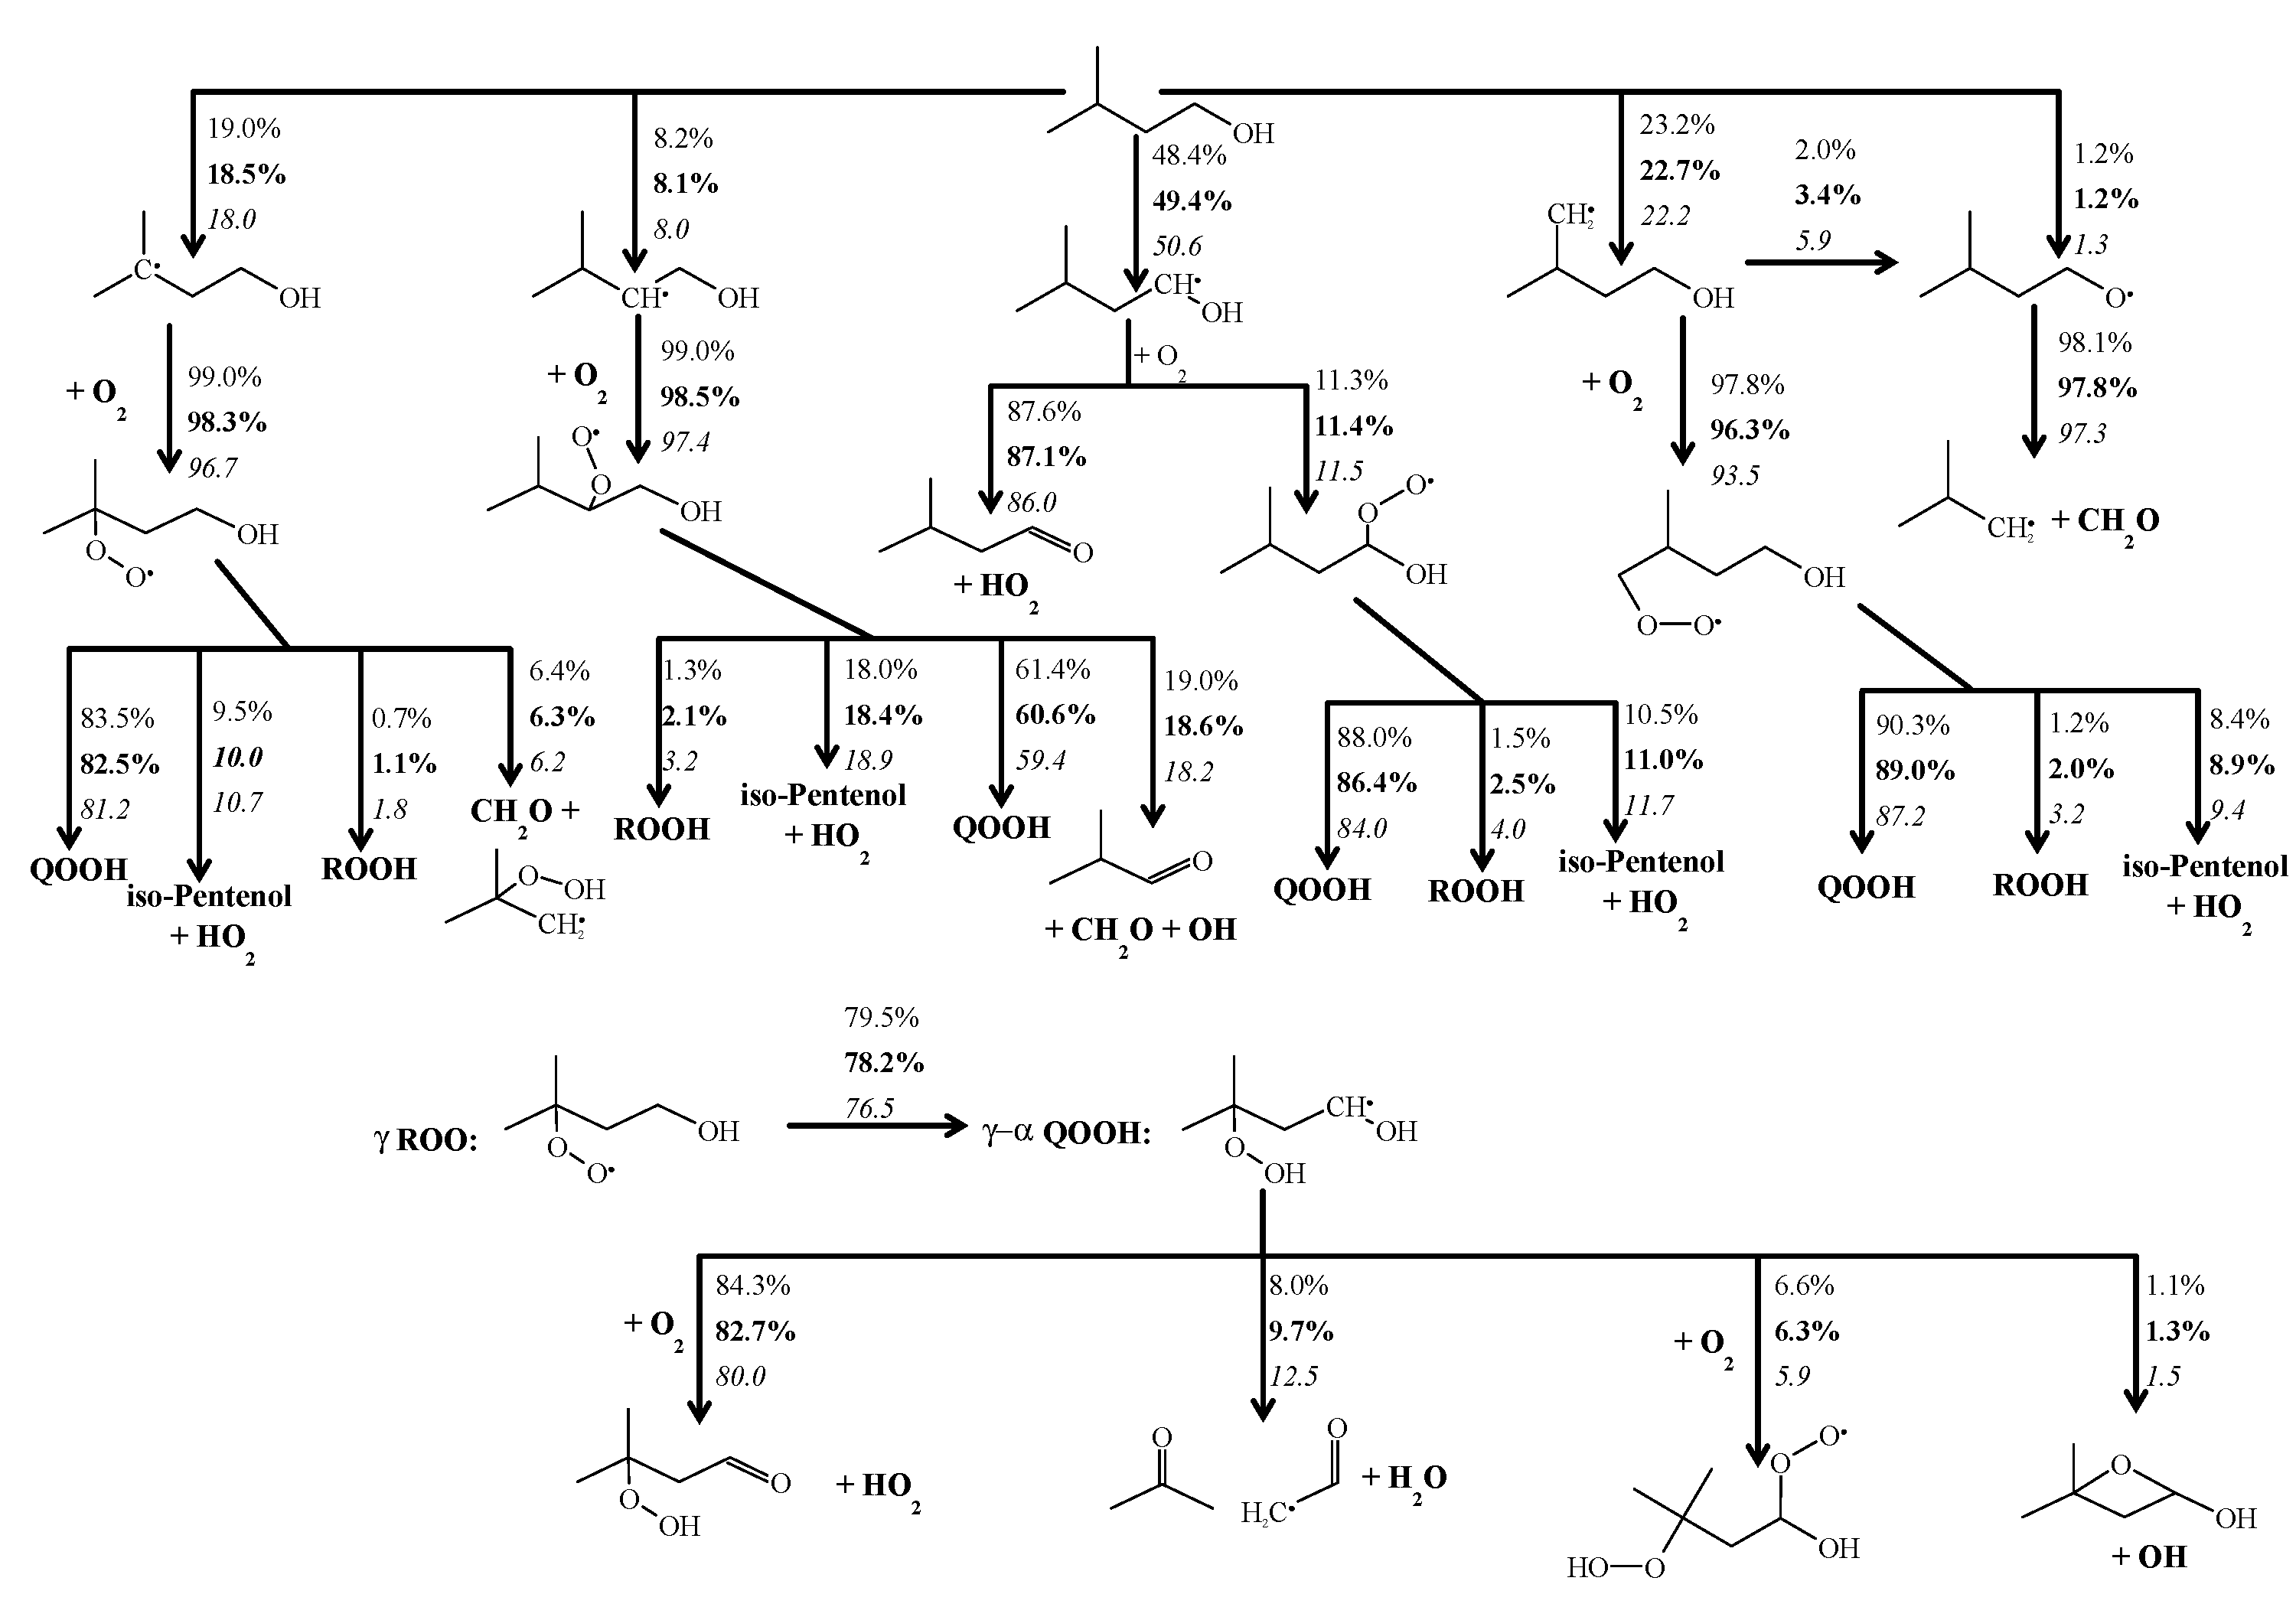
\includegraphics[width=0.89\textwidth]{04-Pentanol/ipeoh-20path}
    \caption{Reaction path analysis for \iPeOH{} at \SI{800}{\kelvin},
    \SI{20}{\atmosphere}, and three equivalence ratios, based on
    constant-volume adiabatic simulations. Plain text: $\phi=0.5$.
    Bold text: $\phi=1.0$. Italic text: $\phi=2.0$. The species flux is
    integrated up to \SI{20}{\percent} fuel consumption.}
    \label{fig:ipeoh-20path}
\end{figure}
\end{landscape}
}

The main \iPeOH{} reaction pathways after \SI{20}{\percent} fuel consumption at
\SI{800}{\kelvin}, \SI{20}{\atmosphere}, and for three equivalence
ratios are shown in \cref{fig:ipeoh-20path}, describing the key low
temperature reaction pathways. The percent flux of each reaction path
is the contribution of that path to destroying the reactant, integrated
up to \SI{20}{\percent} fuel consumption. The fuel is mainly consumed by
the H atom abstraction at the $\alpha$ site because \iPeOH{} has a weak
C-H bond at the $\alpha$ site. As discussed previously, subsequent
reactions of $\alpha$-hydroxypentyl with \ce{O2} generate \textit{i}-pentanal
+ \ce{HO2}, an OH terminating pathway. The other hydroxypentyl radicals tend
to add to molecular oxygen and form hydroxyalkylperoxy (ROO) radicals.
These radicals are mainly isomerized to hydroxyalkylhydroperoxide (QOOH)
or decomposed to enol species by the concerted elimination of \ce{HO2}. Approximately
\SI{18}{\percent} of $\beta$-hydroxyalkylperoxy radicals are decomposed to produce
\textit{i}-butanal (2-methylpropanal), formaldehyde, and OH radical via ROO
isomerization and $\beta$-scission reactions by the Waddington mechanism
\cite{Ray1973, Sway1983}. It is also interesting to note that a similar
pathway involving hydrogen transfer from the OH group is
important for the $\gamma$-ROO (\SI{6}{\percent}) via a 7-membered transition state
ring, which is a reaction sequence we included based on the work
of \textcite{Welz2012}.

\section{Conclusions}
\label{sec:ipeoh-conclusions}

New experimental ignition delay data have been collected in an RCM at
conditions of \SI{40}{\atmosphere}, $\phi=\numrange{0.5}{2.0}$, and
temperatures below \SI{800}{\kelvin}. The measured pressure histories
showed interesting behavior of slow initial pressure rise prior to a
sharp pressure rise indicating overall ignition. This pressure rise
may be attributed to the role of the Waddington mechanism in consuming
the fuel via the production and recycling of OH radicals during the
pre-ignition phase.

An existing model \cite{Tsujimura2012} for \iPeOH{} combustion has been updated with newly
calculated reaction rate coefficients and newly discovered reaction
pathways. The updated model was able to predict the ignition
delays measured in the RCM and STs fairly well, although
it was unable to reproduce the change in reactivity when changing the
equivalence ratio for the low-temperature RCM ignition delay measurements.
The model was also able to qualitatively capture the slow initial pressure
rise measured during the RCM experiments, although the model was unable
to reproduce the quantitative timing of the pressure rise.

Pathway and sensitivity analyses were conducted to understand
the important reactions in the decomposition of \iPeOH{}.
The most important path for consumption of fuel radicals at low
and intermediate temperatures was the reaction of the
$\alpha$-hydroxypentyl radical with \ce{O2} to form
\textit{i}-pentanal and \ce{HO2} , a path that does not contribute to the
low temperature branching. However, sufficient low temperature chain
branching involving the $\gamma$ and $\delta$ fuel radicals occurred
in the model that it was able to reasonably reproduce low-temperature
ignition and reactivity observed in the experiments. Sensitivity
analysis showed that no single reaction can be modified to improve
agreement of the model with all of the conditions, and further
experimental or computational study is required to identify the
cause of the discrepancy in predictions of ignition delay
at off-stoichiometric, low-temperature conditions.
\end{document}


%MCH
% arara: xelatex: { synctex: on, shell: off }
% arara: biber
% arara: xelatex: { synctex: on, shell: off }
% arara: sumatrapdf
\documentclass[12pt, letterpaper]{article}

%Set the document font
\usepackage{fontspec}
\setmainfont[Renderer=Basic,Ligatures=TeX]{Times New Roman}

%Set the size of the margins and the paper
\usepackage[margin=1in, letterpaper]{geometry}

%Set the color of the links and PDF metadata
\usepackage[
    colorlinks=true,
    citecolor=blue,
    linkcolor=black
]{hyperref}

\hypersetup{%
    pdfinfo={
        Title={High Pressure Ignition Chemistry of Alternative Fuels},
        Author={Bryan W. Weber}
    }
}
%Set up the page numbers
%This has to go after geometry so the page number is centered
\usepackage{fancyhdr}
\pagestyle{fancy}
\fancyhf{}
\fancyfoot[C]{\thepage}
\renewcommand{\headrulewidth}{0pt}

%Set a command to easily skip a line
\newcommand{\blankline}{\vspace*{\baselineskip}}

%Set up biblatex
\usepackage[
    backend=biber,
    url=false,
    doi=true,
    sorting=none,
    sortcites=true,
    maxbibnames=6,
    minbibnames=6,
    maxcitenames=2,
    mincitenames=1,
    citestyle=numeric-comp,
    firstinits=true,
    isbn=false
]{biblatex}
\addbibresource{../library.bib}

%Remove the "In:" from before the journal title for articles
\renewbibmacro{in:}{%
  \ifentrytype{article}{}{\printtext{\bibstring{in}\intitlepunct}}}

%Set the sort order of the names in each bibliography entry
\DeclareNameAlias{default}{last-first}

%Don't print the article title. To print the title, add #1 to the last {}
\DeclareFieldFormat[article,incollection,unpublished]{title}{}

%Add Vol. and No. before volume and issue.
\DeclareFieldFormat[article]{volume}{\bibstring{volume}\addspace #1}
\DeclareFieldFormat[article]{number}{\bibstring{number}\addspace #1}

%Put a comma between the volume and issue instead of period
\renewbibmacro*{volume+number+eid}{%
  \printfield{volume}%
  \setunit{\addcomma\space}%<---- was \setunit*{\adddot}%
  \printfield{number}%
  \setunit{\addcomma\space}%
  \printfield{eid}}

%Add a comma after the journal title
\renewbibmacro*{journal+issuetitle}{%
  \usebibmacro{journal}%
  \setunit*{\addcomma\addspace}%
  \iffieldundef{series}
    {}
    {\newunit
     \printfield{series}%
     \setunit{\addspace}}%
  \usebibmacro{volume+number+eid}%
  \setunit{\addspace}%
  \usebibmacro{issue+date}%
  \setunit{\addcolon\space}%
  \usebibmacro{issue}%
  \newunit}

%Set the text to double spacing
\usepackage[doublespacing]{setspace}

%Packages not present in main.tex preamble
\usepackage{booktabs}

\def\chapterautorefname~#1\null{Chap.~#1\null}
\def\sectionautorefname~#1\null{Sec.~#1\null}
\def\subsectionautorefname~#1\null{Sec.~#1\null}
\def\figureautorefname~#1\null{Fig.~#1\null}
\def\tableautorefname~#1\null{Table~#1\null}
\def\equationautorefname~#1\null{Eq.~(#1)\null}

\newcommand{\Autoref}[1]{%
  \begingroup%
  \def\chapterautorefname~##1\null{Chapter~##1\null}%
  \def\sectionautorefname~##1\null{Section~##1\null}%
  \def\subsectionautorefname~##1\null{Sub--Section~##1\null}%
  \def\figureautorefname~##1\null{Figure~##1\null}%
  \def\tableautorefname~##1\null{Table~##1\null}%
  \def\equationautorefname~##1\null{Equation~##1\null}%
  \autoref{#1}%
  \endgroup%
}

\usepackage{caption}
\DeclareCaptionLabelFormat{bf}{\textbf{#1 #2}}
\captionsetup{
    font=small ,
    labelsep=colon ,
    labelformat=bf,
}

\usepackage{subfig}

\usepackage{mathtools}

\usepackage{multirow}

\graphicspath{ {../figures/} }

\newcommand{\linebreakcell}[2][c]{%
  \begin{tabular}[#1]{@{}c@{}}#2\end{tabular}}

\usepackage{siunitx}
\sisetup{%
    group-separator = {,} ,
    range-units = single ,
    range-phrase = {\text{--}} ,
    list-units = single ,
    list-separator = {\text{, }} ,
    list-final-separator = {\text{, and }} ,
}%
\DeclareSIUnit\calorie{cal}

\usepackage{floatrow}
\floatsetup[table]{style=plaintop}

\usepackage{layouts}
%End of extra imports

\begin{document}
\section{Procedures}
\label{sec:mch}

The liquid fuel (methyl-cyclohexane, 99.0\% purity) is massed to a precision
of \SI{0.01}{\gram} in a syringe before being injected into the mixing tank through a
septum. The proportions of oxygen (99.9999\% purity), nitrogen (99.9995\%
purity), and argon (99.9999\% purity) are determined by specifying the oxidizer
composition, the equivalence ratio, and the total mass of fuel. The gases are
added to the mixing tank manometrically at room temperature.

Three different mixtures of MCH/O$_2$/N$_2$/Ar are prepared in this study, as
outlined in \autoref{tab:mch-props}. These mixtures (denoted as Mix \#1–3) match the mixtures
prepared in our previous work with MCH in the RCM \cite{Mittal2009}. The equivalence ratios
corresponding to Mix \#1–3 are $\phi=\numlist{1.0;0.5;1.5}$, respectively.
As in the previous RCM experiments, the mole fraction of MCH is held constant
and the mole fraction of O$_2$ is varied to adjust the equivalence ratio. This
experimental design allows these data to be used to validate chemical kinetic
models for changes in O$_2$ concentration, which is an important variable in
internal combustion engines where exhaust gas recirculation is used to reduce
the oxygen concentrations to avoid NOx formation. Few validation data for
ignition are available for changing oxygen concentrations. In addition, the
relative proportions of O$_2$, N$_2$, and Ar are adjusted so that the same specific
heat ratio is maintained in the three mixtures. The utility of this
experimental design will be discussed in due course.

\begin{table}
    \caption{Molar Proportions of Reactants in MCH Experiments}
    \label{tab:mch-props}
    \begin{tabular}{*{6}{S}}
    \toprule
    {Mix \#} & {$\phi$} & {MCH} & {O$_2$} & {N$_2$} & {Ar} \\
    \midrule
    1 & 1.0 & 1 & 10.5 & 12.25 & 71.75 \\
    2 & 0.5 & 1 & 21.0 &  0.00 & 73.50 \\
    3 & 1.5 & 1 &  7.0 & 16.35 & 71.15 \\
    \bottomrule
    \end{tabular}
\end{table}

\section{Model Improvements}
\label{sec:model-improvements}

Through collaboration with researchers at Lawrence Livermore National
Laboratories, many improvements to the chemical kinetic model for MCH were
made. Some of the major improvements are highlighted below; see the article
for more detail. It should be noted that the improvement relative to the model
from 2007 by \textcite{Pitz2007} is substantial.

\begin{enumerate}
    \item The base C$_1$--C$_4$ chemistry has been updated with the AramcoMech
        version 1.3 \cite{Metcalfe2013}
    \item The aromatics base chemistry was updated with the latest LLNL-NUIG
        model \cite{Nakamura2014}
    \item The cyclohexane sub-model was updated with a new version from
        \textcite{Silke2007}
    \item Rates of abstraction reactions from MCH have been updated
        with recently measured experimental values \cite{Sivaramakrishnan2009}
        and standardized according to the LLNL reaction rate rules \cite{Sarathy2011b}
    \item Products of MCH breakdown with unsaturated rings such as
        methylcyclohexene were previously lumped into one species for
        simplicity. In the new model, they have been unlumped and
        provide improved fidelity in modeling these species. \cite{Pitz2013}
    \item The reaction rates of some low-temperature specific reactions were
        updated using new quantum chemical calculations to compute the rate.
        Other reaction rates were updated from similar calculations performed
        by \textcite{Fernandes2009}
    \item The activation energy of the ketohydroperoxide decomposition
        reactions was increased to bring it into closer agreement with
        the activation energy used by \textcite{Metcalfe2013}. This change
        has a dramatic effect on the low-temperature ignition delays, as shown
        in \autoref{sec:model-comparison}.
\end{enumerate}

\section{Experimental Results}
\label{sec:experimental-results}

The experimental ignition delays measured at the three equivalence ratios and
compressed pressure of \SI{50}{\bar} are shown in \autoref{fig:mch-expts}. The open symbols are the
overall ignition delays and the filled symbols are the first stage ignition
delays. The vertical error bars on the experimental data represent twice the
standard deviation of all of the experiments at that condition. Detailed
uncertainty analysis of the deduced compressed temperature was conducted
in \autoref{sec:uncertainty} where the maximum uncertainty of the compressed
temperature was found to be approximately $\pm 1\%$.

The negative temperature coefficient (NTC) region is an important feature of
low temperature ignition where the ignition delay time increases with
increasing temperature. The NTC region of the overall ignition delay is
evident in \autoref{fig:mch-expts} for the $\phi=\num{1.5}$ case (Mix \#3) and
approximately includes the temperature range of $T_C=\SIrange{775}{840}{\kelvin}$. For
$\phi=\num{1.5}$, first stage ignition is evident for conditions in the range of
$T_C=\SIrange{740}{800}{\kelvin}$.

For $\phi=\num{1.0}$ (Mix \#1), the NTC region of the overall ignition delay could
not be completely resolved. Only three conditions in the low temperature region
and three conditions in the high temperature region are shown in
\autoref{fig:mch-expts}. The experimental pressure traces during the compression
stroke for intermediate temperature conditions were seen to deviate from their
non-reactive counterparts, demonstrating appreciable reactivity therein. Hence,
those data are not included in \ref{fig:mch-expts}.

For the experiments at $\phi=\num{0.5}$ (Mix \#2), only three data points in the low
temperature region are reported and none of them exhibits two-stage ignition
response. As the temperature is increased further, noticeable reactivity during
the compression stroke is evident.

As stated earlier, the mole fraction of MCH is held constant in this study,
while the mole fraction of the oxidizer is changed to modify the equivalence
ratio. \Autoref{fig:mch-expts} demonstrates that the $\phi=\num{0.5}$ case is the most
reactive (as judged by the inverse of the ignition delay) and the $\phi=\num{1.5}$
case is the least reactive. As has been shown for other fuels, including
\textit{n}-butanol \cite{Weber2011} and Jet-A \cite{Kumar2010}, decreasing the
equivalence ratio by increasing the oxygen mole fraction but holding the fuel
mole fraction constant increases the reactivity.

\section{Comparison to Model}
\label{sec:model-comparison}

A comparison of the experimentally measured first stage ignition delays (open
symbols) and the first stage ignition delays computed using the updated model
(lines) is shown in Figs. (\ref{fig:mch-model-1}a), (\ref{fig:mch-model-2}a),
and (\ref{fig:mch-model-3}a) for Mix \#1, \#2, and \#3, respectively. In
addition, a comparison of the experimentally measured overall ignition delays
(open symbols) and the overall ignition delay computed by the updated model
(lines) is shown in Figs. (\ref{fig:mch-model-1}b), (\ref{fig:mch-model-2}b),
and (\ref{fig:mch-model-3}b). The experiments include the new work being
presented here at $P_C=\SI{50}{\bar}$ in addition to the previous RCM experiments at
$P_C=\SIlist{15.1;25.5}{\bar}$ \cite{Mittal2009}. The simulations are the VPRO type
of simulations. For some computational cases, substantial heat release during
the compression stroke caused the computed pressure to depart from the
non-reactive profile prior to EOC. Therefore, these cases are not shown in
Figs. (\ref{fig:mch-model-1})--(\ref{fig:mch-model-2}). For these conditions, the
experimental pressure trace did not exhibit significant heat release during
the compression stroke and the experimental pressure at EOC for the reactive
case matched that of the non-reactive counterpart.

\begin{figure}
    \begin{floatrow}
        \ffigbox
            {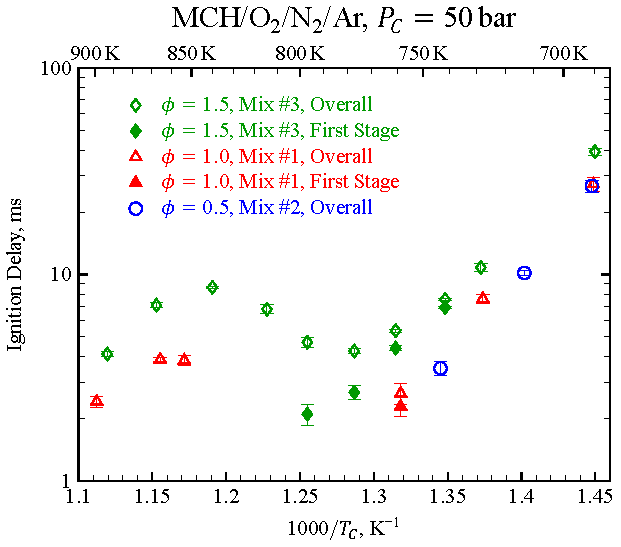
\includegraphics[width=7.9cm]{05-MCH/mch-expts}}
            {\caption{Experimentally measured ignition delays at $P_C=\SI{50}{\bar}$ for the
                mixture conditions in \autoref{tab:mch-props}}
            \label{fig:mch-expts}}
        \ffigbox
        {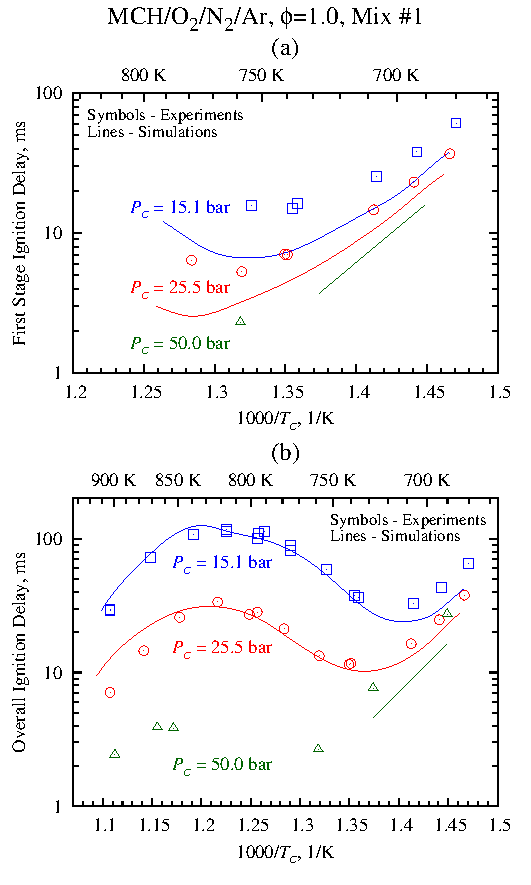
\includegraphics[width=7.9cm]{05-MCH/mch-model-1}}
            {\caption{Comparison of experimental and simulated ignition delays for three
                pressures for Mix \#1. The data at \SIlist{15.1;25.5}{\bar} are from the
                study of \textcite{Mittal2009}. (a) First stage ignition delays,
                (b) overall ignition delays.}
            \label{fig:mch-model-1}}
    \end{floatrow}
\end{figure}

\begin{figure}
    \begin{floatrow}
        \ffigbox
            {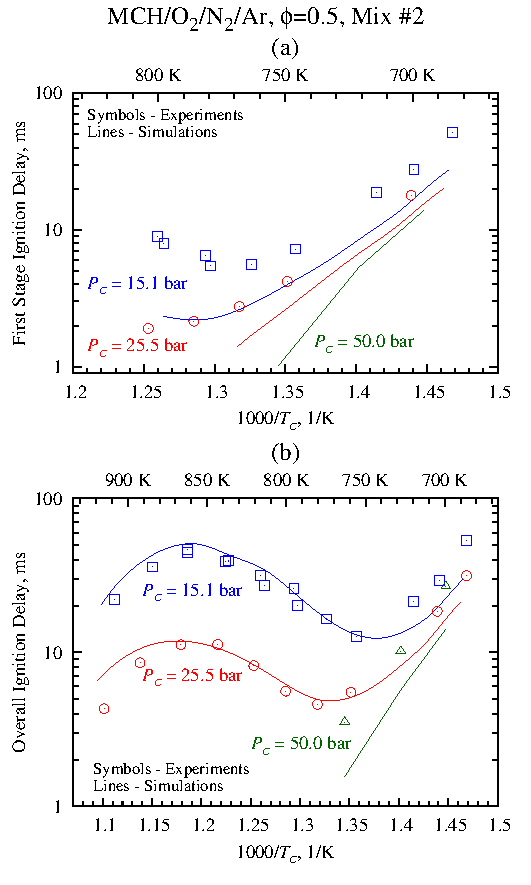
\includegraphics[width=8cm]{05-MCH/mch-model-2}}
            {\caption{Comparison of experimental and simulated ignition delays for three
                pressures for Mix \#2. The data at \SIlist{15.1;25.5}{\bar} are from the
                study of \textcite{Mittal2009}. (a) First stage ignition delays,
                (b) overall ignition delays.}
            \label{fig:mch-model-2}}
        \ffigbox
            {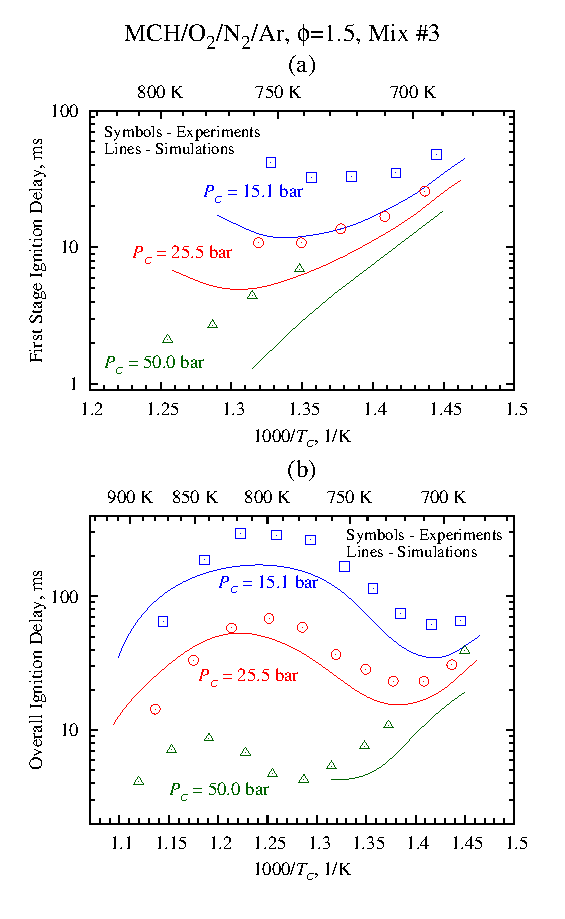
\includegraphics[width=8cm]{05-MCH/mch-model-3}}
            {\caption{Comparison of experimental and simulated ignition delays for three
                pressures for Mix \#3. The data at \SIlist{15.1;25.5}{\bar} are from the
                study of \textcite{Mittal2009}. (a) First stage ignition delays,
                (b) overall ignition delays.}
            \label{fig:mch-model-3}}
    \end{floatrow}
\end{figure}

At \SIlist{15.1;25.5}{\bar} for Mix \#1 and \#2, the overall ignition delay is very
well predicted for temperatures above approximately \SI{715}{\kelvin}. For lower
temperatures at these two equivalence ratios, the experimental ignition delays
are under-predicted by the model, but the predictions are nevertheless within
a factor of two of the data. For the rich case (Mix \#3), the simulations
under-predict the ignition delay over a wider temperature range but the results
improve as temperature increases. Again, the experimental ignition delays are
predicted to within approximately a factor of two. At \SI{50}{\bar}, the ignition
delays are under-predicted for all of the equivalence ratios studied here, but
the agreement is within a factor of two.

The first stage ignition delays for all of the pressure and equivalence ratios
are under-predicted, but are within a factor of three of the experimental
values. Furthermore, for all of the equivalence ratios tested at $P_C=\SI{50}{\bar}$,
it is of interest to note that there are several cases where simulated ignition
delays show two-stage response where the experiment shows only a single stage
ignition. Nevertheless, the present mechanism is a marked improvement from the
comparison performed by \textcite{Mittal2009} who found that the ignition
delays were strongly and uniformly over-predicted by the previous LLNL
mechanism by \textcite{Pitz2007}.

\Autoref{fig:mch-pressure}(a)--(c) shows a comparison of selected simulated and
experimentally measured pressure traces for Mix \#1, \#2, and \#3,
respectively, at $P_C=\SI{50}{\bar}$. Also shown in \autoref{fig:mch-pressure} is the
simulated non-reactive pressure trace corresponding to each experimental
condition. Small differences in the heat loss profile for different
temperatures are apparent in the non-reactive pressure traces. These
differences arise from the changing surface area to volume ratio of the
reaction chamber at the end of compression as the compression ratio is changed
to vary the compressed temperature. This highlights the importance of using
VPRO simulations to compare predictions of ignition delay with the experimental data.

For Mix \#1, it is clear that the simulated reactive pressure trace in
\autoref{fig:mch-pressure}(a) at $T_C=\SI{866}{\kelvin}$ (red dashed line) deviates from
the non-reactive pressure trace (red dot-dot-dashed line) prior to the end of
compression. The same is also true of the \SI{797}{\kelvin} case shown for Mix \#3 in
\autoref{fig:mch-pressure}(c). Remarkably, the simulated case for Mix \#1 at
$T_C=\SI{866}{\kelvin}$ predicts the overall ignition delay quite well. However, due to the
heat release prior to EOC, this simulated result is not plotted in
\autoref{fig:mch-model-1}. The simulated case for Mix \#3 at $T_C=\SI{797}{\kelvin}$ is also
not plotted on \autoref{fig:mch-model-3} due to the heat release prior to EOC;
interestingly, this case under-predicts the first stage ignition delay but
over-predicts the overall ignition delay. For the other simulated cases (black
lines), the reactive pressure traces closely follow their non-reactive
counterparts until the ignition event begins. The experimental ignition delays
of these cases are under-predicted by the model. It is also seen in
\autoref{fig:mch-pressure}(c) for $T_C=\SI{729}{\kelvin}$ that the model predicts two-stage
ignition, although two-stage ignition is not observed experimentally.

\begin{figure}
    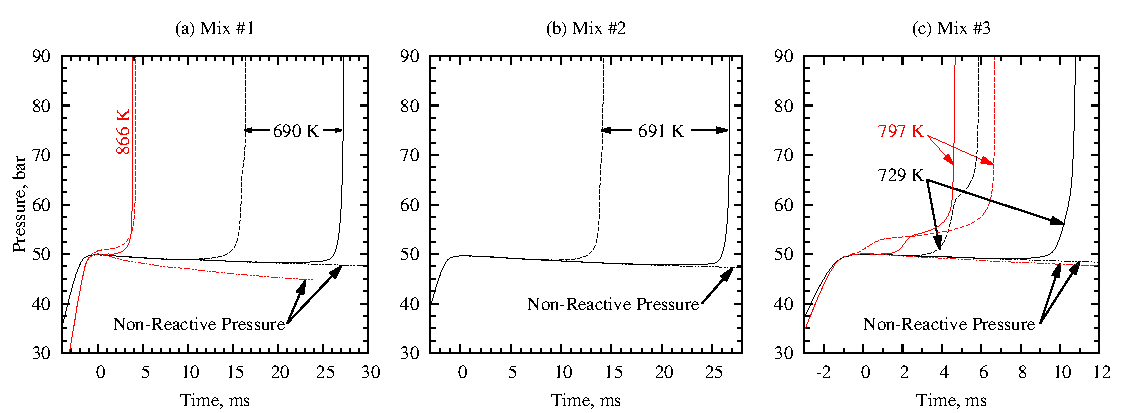
\includegraphics[width=\textwidth]{05-MCH/mch-pressure}
    \caption{Comparison of selected simulated and experimental pressure traces
        at $P_C=\SI{50}{\bar}$ for (a) Mix \#1 (b) Mix \#2 (c) Mix \#3. Red lines
        indicate that the pressure profile of the reactive simulation deviates
        from the non-reactive case prior to EOC. Solid lines: experiment;
        dashed lines: reactive simulation; dot-dot-dashed lines: non-reactive
        simulation.}
    \label{fig:mch-pressure}
\end{figure}

The current mechanism is also compared to shock tube ignition delays from the
studies of \textcite{Vasu2009} and \textcite{Vanderover2009}. Those studies
considered the autoignition of stoichiometric mixtures of MCH with O$_2$/N$_2$
air. The comparison is shown in \autoref{fig:mch-shocks} for the near \SI{50}{atm}
data from those studies. Note that the experimental data shown are the raw
data and are not scaled to a constant pressure, whereas the simulated
ignition delays are at a constant initial pressure of \SI{50}{atm}. It can be seen
that the ignition delays are over-predicted over the nearly entire temperature
range of \SIrange{795}{1160}{\kelvin} studied. Nevertheless, the predicted ignition delays are
within approximately a factor of 1.5 of the experiments, indicating good
agreement overall and a substantial improvement from the previous version of
the model. Furthermore, the simulations shown here are of the CONV type and
do not account for any facility dependent effects present in the experiments.
Although the experimentalists noted in \cite{Vasu2009,Vanderover2009} that the
effect of such considerations is minimal in their studies, including facility
dependent effects will tend to make the simulations ignite sooner and improve
the agreement, especially for cases with ignition delays longer than
approximately \SI{1000}{\micro\second}.

As discussed in \autoref{sec:model-comparison}, one of the updates to the model
was to increase the activation energy of ketohydroperoxide decomposition, from
$E_a=\SI{39}{\kilo\calorie\per\mole}$ (\SI{163.2}{\kilo\joule\per\mole}) to
\SI{41.6}{\kilo\calorie\per\mole} (\SI{174.1}{\kilo\joule\per\mole}). This
update substantially improved the prediction of the low-temperature ignition
delays, including the first stage and overall ignition delays. As mentioned by
\textcite{Curran2002}, "the high activation energy [of ketohydroperoxide
decomposition] ensures an induction period during which the ketohydroperoxide
concentration builds up." Furthermore, updating this activation energy does not
affect the high-temperature ignition delays. A comparison of calculated
ignition delays demonstrating the effect of this update is shown in
\autoref{fig:mch-energy}.

\begin{figure}
    \begin{floatrow}
        \ffigbox
            {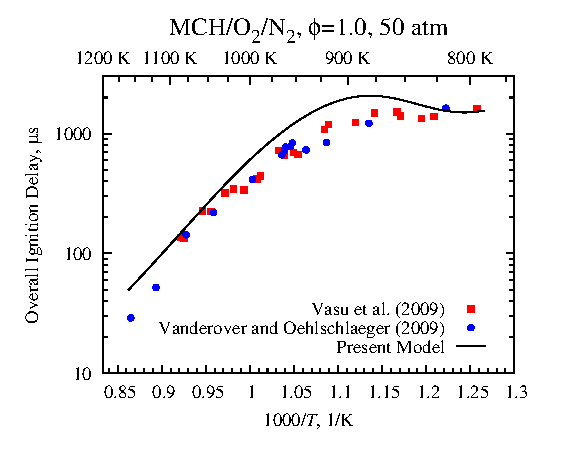
\includegraphics[width=7.9cm]{05-MCH/mch-shocks}}
            {\caption{Comparison of the present model with the experiments from
                \textcite{Vasu2009} and \textcite{Vanderover2009} near \SI{50}{atm}
                and for stoichiometric mixtures in O$_2$/N$_2$ air.}
            \label{fig:mch-shocks}}
        \ffigbox
            {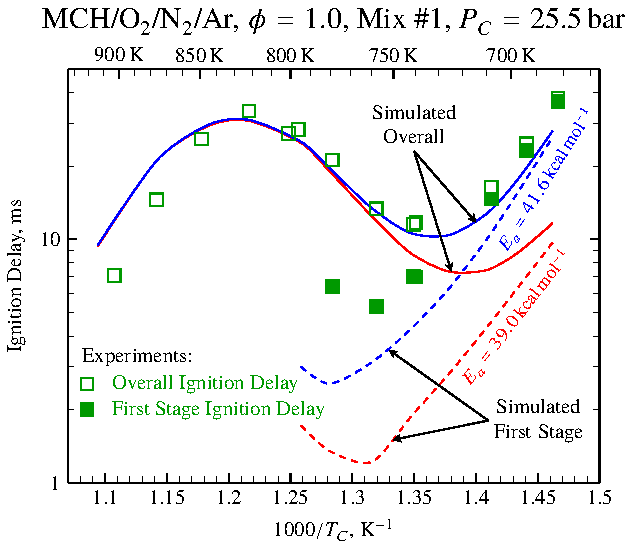
\includegraphics[width=7.9cm]{05-MCH/mch-energy}}
            {\caption{Comparison of mechanism performance with the activation energy
                of ketohydroperoxide decomposition set at \SI{41.6}{\kilo\calorie\per\mole} (blue) and
                \SI{39.0}{\kilo\calorie\per\mole} (red). Experimental ignition delays are shown in
                green symbols.}
            \label{fig:mch-energy}}
    \end{floatrow}
\end{figure}

\section{Discussion}
\label{sec:discussion}
\subsection{Path Analysis}
\label{sec:mch-path-analysis}

The relatively good agreement of the updated model with the experimental data
suggests that a more detailed analysis of the mechanism is a worthwhile
exercise and such analysis may point the way to further improvements to the
mechanism. We begin with a reaction path analysis. The present reaction path
analysis is conducted using a CONV (adiabatic, constant-volume) type simulation
for three initial temperatures (\SIlist{700;800;900}{\kelvin}), at \SI{25.5}{\bar} and for
Mix \#1 (the stoichiometric case). For the other mixture conditions and
pressures considered in this work, the absolute percentages for each channel
change slightly. However, the analysis of the reaction pathways is the same for
all of the equivalence ratios and pressures considered in the experiments
presented previously. The three temperatures considered in this analysis
correspond to the low-temperature, peak of the NTC, and high-temperature
portions of the ignition delay curve illustrated in \autoref{fig:mch-energy};
their results are shown in \autoref{fig:mch-path} with plain text, bold text,
and italic text, respectively.

The path analysis presented in \autoref{fig:mch-path} is an integrated analysis
where the rate of production (ROP) of each species by each reaction has been
integrated with respect to time up to 20\% fuel consumption. The integrated
ROPs from each reaction are normalized by the total production or destruction
of that species up to 20\% fuel decomposition, such that reactions that produce
a species are normalized by the total production of the species and reactions
that consume a species are normalized by the total consumption of that species.
The percentages in \autoref{fig:mch-path} therefore represent the percent of the given
reactant that is consumed to form the given product by all reactions that can
form a particular product. Species such as hydroperoxyalkyl radicals (QOOH),
alkyl hydroperoxides (ROOH), and methylcyclohexenes (MCH-ene) are shown as
lumped on the path diagram; however, these species are unlumped in the
mechanism and presented as a lumped sum for simplicity in this diagram. Note
that not all of the pathways present in the mechanism for each species are
presented in \autoref{fig:mch-path}, again for simplicity; the pathways that are shown in
\autoref{fig:mch-path} typically account for more than 95\% of the consumption
of each species.

\begin{figure}
    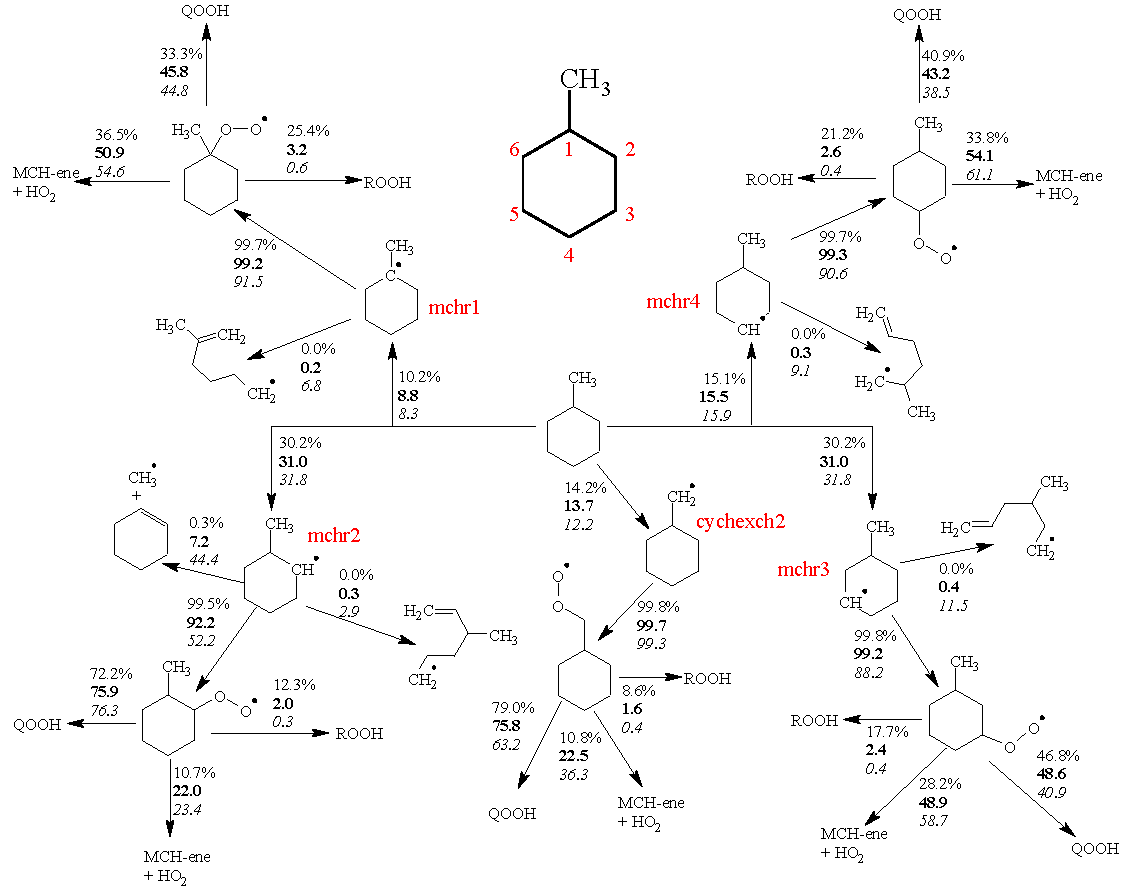
\includegraphics[width=\textwidth]{05-MCH/mch-path}
    \caption{Path analysis of MCH combustion. Initial conditions are 25.5 bar
    and Mix \#1 ($\phi=\num{1.0}$) and \SI{700}{\kelvin} (plain text),
    \SI{800}{\kelvin} (bold text), \SI{900}{\kelvin} (italic text).
    Note that not all possible reaction pathways are shown for
    each species.}
    \label{fig:mch-path}
\end{figure}

The first step of fuel breakdown occurs by H-atom abstraction at these pressure
and temperature conditions. None of the fuel is directly decomposed by
unimolecular reactions. Each of the seven possible radicals are formed in
comparable quantities; however, due to the symmetry of MCH, sites 2 and 3 are
equivalent to sites 6 and 5, respectively, so mchr2 and mchr3 have close to
double the production rate compared to the other radicals. It is interesting to
note that the production of mchr2, mchr3, and mchr4 increase as the initial
temperature increases and the production of mchr1 and cychexch2 decrease to
compensate. However, the change is small, no more than 2 percentage points for
each radical.

The most important second step is oxygen addition (i.e. formation of ROO) at
all of the initial temperatures in this analysis. The importance of this
reaction diminishes for each radical as the initial temperature increases due
to the increasing importance of $\beta$-scission reactions. At \SI{700}{\kelvin}, less than
0.05\% of each of the fuel radicals is consumed via $\beta$-scission. Between
\SIlist{800;900}{\kelvin}, the percentages of mchr1, mchr2, mchr3, and mchr4 that are decomposed
via $\beta$-scission increase by several thousand percent each; nevertheless,
the absolute change is small and the consumption of these radicals still occurs
mostly by oxygen addition. The mchr1, mchr3, and mchr4 radicals undergo
scission of the cyclohexyl ring, whereas mchr2 primarily scissions at the
methyl-cyclohexyl bond. This beta scission of mchr2 competes significantly with
its consumption by O$_2$ at \SI{900}{\kelvin}. Furthermore, the increasing importance of the
ring opening reactions from \SI{800}{\kelvin} to \SI{900}{\kelvin} means that chain propagation pathways
(instead of effective chain termination pathways forming methylcyclohexene and
hydroperoxyl) are available, increasing the reactivity. Finally, even at the
elevated initial temperature of \SI{900}{\kelvin}, cychexch2 does not undergo significant
ring opening. Instead, it will scission an H atom from site 1 or steal an oxygen
atom from hydroperoxyl to form an alkoxy radical (RO) when it does not undergo
oxygen addition (these pathways each only consume about 0.3\% of cychexch2 and
hence are not shown in \autoref{fig:mch-path}).

Returning to the low temperature pathways, there are four important classes of
reactions that consume the ROO radicals in the current mechanism. These classes
are: C1) internal H-atom transfer (isomerization) to form QOOH; C2) direct
elimination of hydroperoxyl and methylcyclohexene; C3) H-abstraction by ROO
from either the fuel or hydroperoxyl to form ROOH; and, C4) reactions among the
ROO radicals. Class C4 consumes less than ~5\% of each of the ROO radicals at
\SI{700}{\kelvin} and less than ~0.1\% for the other temperatures and this class is
therefore not shown on the path diagram in \autoref{fig:mch-path}. Of the other
three classes, C1 (formation of QOOH) is the predominant pathway in the low
temperature ignition process. Nevertheless, the direct elimination of
methylcyclohexene and hydroperoxyl and the formation of ROOH are important at
low temperatures as well.

For all of the temperatures considered here, a majority of the ROOH is formed
by reactions of ROO with hydroperoxyl to give ROOH and an oxygen molecule. At
the initial temperature of \SI{700}{\kelvin}, approximately 15\% of the fuel reacts to form
ROOH, indicating its importance in low-temperature MCH combustion. The primary
route of ROOH formation in this mechanism (H-abstraction from hydroperoxyl by
ROO) has not been well studied at combustion relevant temperatures
\cite{Zador2011} and is therefore a good candidate for further investigation
given its importance in the model for MCH combustion.

As the temperature increases, the formation of ROOH becomes substantially less
important while the direct HO$_2$ elimination reaction becomes more important.
The increase in production of methylcyclohexene and hydroperoxyl plays a role
in the NTC region of ignition delay because this is effectively a chain
terminating channel until the temperature increases enough that the sequence
MCH+HO$_2$=R+H$_2$O$_2$; H$_2$O$_2$(+M)=2OH(+M) becomes important and drives
the overall ignition.

Interestingly, for most of the ROO radicals, the change in the fraction of ROO
consumed to form QOOH is non-monotonic as temperature increases. That is, for
mch1oo, mch3oo, and mch4oo the production of QOOH increases in going from \SI{700}{\kelvin}
to \SI{800}{\kelvin}, then decreases going from \SI{800}{\kelvin} to \SI{900}{\kelvin} due to the increasing
importance of the HO$_2$ elimination channel (due to nuances in the various
reaction paths, mch2oo and chxch2oo do not follow this trend). Furthermore,
the branching ratios in the decomposition of the QOOH species change as the
temperature is increased (not shown in \autoref{fig:mch-path}). At the lowest
temperature (\SI{700}{\kelvin}), the formation of hydroperoxyalkylperoxy radicals (OOQOOH)
is favored, leading to low-temperature chain branching and the two-stage
ignition phenomenon. However, at \SI{800}{\kelvin} and \SI{900}{\kelvin}, the QOOH tends to decompose
into a heptenone and a hydroxyl radical, or one of two epoxide species. Due to
the apparent importance of these species in the intermediate temperature
decomposition of MCH, further investigation of their pathways is warranted.

\subsection{Sensitivity Analysis}
\label{sec:mch-sensitivity-analysis}

Our second type of analysis is a brute force, one-at-a-time sensitivity
analysis. In this work, the sensitivity of the ignition delay to the reaction
rates is considered. Due to the size of the mechanism, only the reactions of
the fuel and the fuel radicals up to the OOQOOH species are considered. This
approach is justified because many of the reactions of the C0-C4 base
mechanism are known to be important to the ignition process (e.g.,
H$_2$O$_2$(+M)=2OH(+M)), but we are more interested in the effect of updates to
the fuel specific sub-mechanism. The sensitivity index is defined in
\autoref{eq:mch-sens},
%
\begin{equation}
    \label{eq:mch-sens}
    S_i = \frac{\ln\left(\tau_{i,2}/\tau_{i,1}\right)}{\ln\left(k_{i,2}/k_{i,1}\right)}
\end{equation}
%
where $\tau$ is the ignition delay time, either first stage or overall, $k$ is
the reaction rate, and subscript $i$ indicates the reaction number. The
numbered subscripts in \autoref{eq:mch-sens} indicate the type of modification
that has been made to the rate of reaction $i$ when computing the ignition
delay, as discussed in the following.

The reaction rates are modified by multiplying and dividing the pre-exponential
constant by a factor $f$. Thus, the forward and reverse rates are
simultaneously modified. Special care is taken to properly modify reaction
rates with pressure dependence and explicit reverse parameters. Each rate is
modified sequentially and the ignition delay is computed; the pre-exponential
constant is reset to its nominal value before modifying the next reaction.
Finally, the nominal ignition delay with no rate modification is computed.
Thus, each set of reactor input conditions requires $2N+1$ model evaluations,
where $N$ is the number of reactions considered in the sensitivity analysis
and $N$ may be less than or equal to the total number of reactions.

The $2N+1$ model evaluations result in $4N+2$ ignition delays if two-stage
ignition is present and $2N+1$ ignition delays otherwise. These ignition delays
are used to compute the sensitivity indices according to \autoref{eq:mch-sens}.
In the case of bidirectional sensitivity indices, the subscript $2$ in
\autoref{eq:mch-sens} is associated with multiplication by $f$ and the subscript
$1$ is associated with division by $f$, resulting in $2N$ sensitivity indices if
two-stage ignition is present and $N$ indices otherwise. In the case of
unidirectional sensitivity indices, the subscript $2$ is associated with either
multiplication or division by $f$ and the subscript $1$ is associated with the
nominal ignition delay, $\tau_{i,1}=\tau_1$. For unidirectional sensitivity
indices, $4N$ indices are obtained if two-stage ignition is present and $2N$ are
obtained otherwise.

In this work, the bidirectional sensitivity is used with $f=10$. For all of the
reactions considered here, multiplying and dividing a given rate had opposite
effects on the ignition delay. Thus, if the ignition delay increased (relative
to the nominal case) when the rate of a certain reaction was multiplied, the
ignition delay decreased (relative to the nominal case) when the rate of the
same reaction was divided and vice versa. Since $k_{i,2}$ is greater than
$k_{i,1}$ by definition, the sensitivity index $S_i$ will be positive if
$\tau_{i,2}>\tau_{i,1}$ (i.e. increasing the rate increases the ignition delay)
and negative if $\tau_{i,2}<\tau_{i,1}$ (i.e. increasing the rate decreases the
ignition delay). The sensitivity analysis is run at the same conditions of the
path analysis: CONV simulation, initial temperatures of \SIlist{700;800;900}{\kelvin},
initial pressure of \SI{25.5}{\bar}, and Mix \#1. As with the path analysis, similar
results are obtained for other pressures and mixtures.

\Autoref{fig:mch-sens} shows the sensitivity indices for the five reactions
(among all the reactions considered in the present sensitivity analysis) to
which the overall ignition delay is most sensitive for each temperature studied
(\SIlist{700;800;900}{\kelvin}). For the results at \SIlist{700;800}{\kelvin}, the
bidirectional sensitivity of the first stage ignition delay to the same
reactions is also shown, except for two reactions at \SI{800}{\kelvin} for which the
unidirectional sensitivity is plotted. The reasons for this will be discussed
in due course. It should be noted that the sensitivity indices of the first
stage ignition delay have a slightly different ranking than the indices of the
overall ignition delay. Therefore, the rank of the first stage sensitivity
index of the reactions shown is given in parentheses next to the bar. At \SI{700}{\kelvin},
the sensitivity of the overall ignition delay is in red and the sensitivity of
the first stage ignition delay is in blue; at \SI{800}{\kelvin}, the sensitivity of the
overall ignition delay is in grey and the sensitivity of the first stage
ignition delay is in green. The most sensitive reaction affecting the first
stage ignition delay at \SI{800}{\kelvin} is found to be MCH+OH=mchr3+H2O, although it is
not listed in \autoref{fig:mch-sens}. At \SI{900}{\kelvin}, there is no first stage
ignition, and thus no sensitivity of the first stage ignition delay.

Under the pressure/stoichiometry conditions of the present simulations, \SI{800}{\kelvin}
is approximately the highest initial temperature at which distinct two-stage
ignition (i.e. two inflection points in the temperature or pressure trace) is
found for MCH with the current mechanism. As such, several reactions affect
the ignition strongly enough to eliminate the first inflection point. These
reactions are given in \autoref{tab:mch-sens} for either multiplication or
division of the rate by the factor $f=10$. The naming convention of the species
listed in \autoref{tab:mch-sens} can be found in \autoref{fig:mch-path},
\autoref{fig:mch-species}, and \autoref{app:mch-dict}. Two reactions shown in
\autoref{tab:mch-sens} also appear in \autoref{fig:mch-sens}, namely (R1)
mch2oo=mch2ene+ho2 and (R2) mch2qx+o2=mch2qxqj. For these reactions at \SI{800}{\kelvin},
the unidirectional sensitivity index is shown in \autoref{fig:mch-sens}, where $\tau_{i,2}$
in \autoref{eq:mch-sens} is found by division of the rate for $i=R1$ and by
multiplication of the rate for $i=R2$.

The role of the ROO=methylcyclohexene+HO$_2$ reactions in the left column of
\autoref{tab:mch-sens} in eliminating the first stage of ignition is clear ---
this set of reactions diverts ROO radicals from entering the low-temperature
chain branching pathway via QOOH that leads to the two-stage ignition.
Similarly, in the right column, decreasing the rate of the reaction of oxygen
with QOOH to form OOQOOH reduces the rate of chain branching that leads to
two-stage ignition. Concerning the reactions of the fuel with OH in the left
column of \autoref{tab:mch-sens}, increasing these rates increases the
formation of fuel radicals that are less reactive at low temperature than the
cychexch2 and mchr2 radical. For example, the mchr2 radical adds to O$_2$ and
forms a peroxy radical (mch2oo) that has a fast RO2 isomerization path to QOOH
involving the abstraction of an H atom from the methyl group. This ROO
isomerization is the path calculated and discussed in Section 4.1 of
\cite{Weber2014}. QOOH subsequently adds to O$_2$ and leads to chain branching.
The high reactivity of cychexch2 and mchr2 at low temperature is reflected by
the high percentages at \SI{800}{\kelvin} (>70\%) leading to QOOH from cychexch2oo and
mch2oo in \autoref{fig:mch-path}.

\begin{table}
    \caption{Reactions that eliminate the first inflection point for a nominal
    case with two-stage ignition.}
    \label{tab:mch-sens}
    \begin{tabular}{c c}
    \toprule
    Multiplication & Division \\
    \midrule
    mch2oo = mch2ene + ho2 & mch2qx + o2 = mch2qxqj \\
    mch3oo = mch2ene + ho2 & \\
    mch3oo = mch3ene + ho2 & \\
    mch + oh = mchr1 + h2o & \\
    mch + oh = mchr4 + h2o & \\
    mch + oh = mchr3 + h2o & \\
    \bottomrule
    \end{tabular}
\end{table}

\begin{figure}
    \begin{floatrow}
        \ffigbox
            {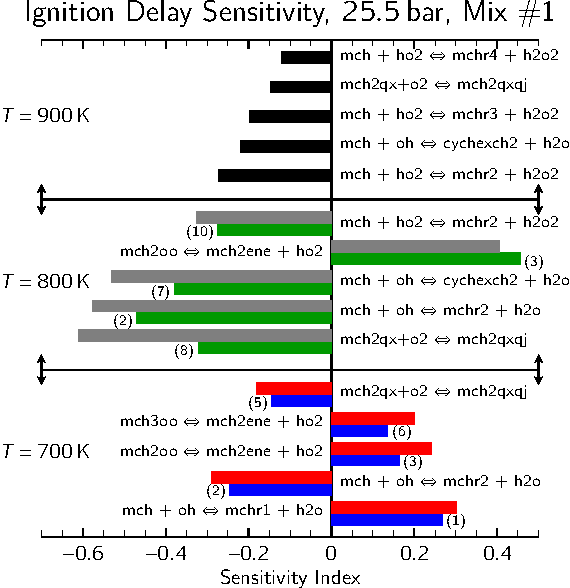
\includegraphics[angle=-90, width=8cm]{05-MCH/mch-sens}}
            {\caption{Sensitivity of the ignition delay to various reaction rates
                for Mix \#1 ($\phi=\num{1.0}$), \SI{25.5}{\bar} and three temperatures
                (\SIlist{700;800;900}{\kelvin}). At \SI{700}{\kelvin}, the sensitivity of the overall
                ignition delay is in red and the sensitivity of the first stage
                ignition delay is in blue. At \SI{800}{\kelvin}, the sensitivity of the overall
                ignition delay is in grey and the sensitivity of the first stage
                ignition delay is in green. At \SI{900}{\kelvin}, the sensitivity of the overall
                ignition delay is in black. Numbers in parentheses represent the
                ranking of the first stage sensitivity indices.}
            \label{fig:mch-sens}}
        \ffigbox
            {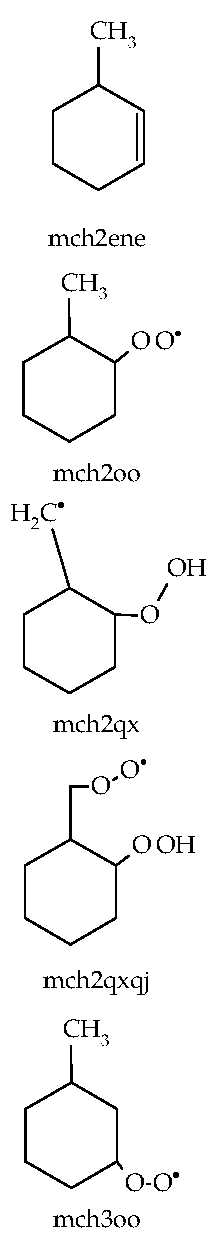
\includegraphics[width=8cm]{05-MCH/mch-species}}
            {\caption{Species mentioned in \autoref{fig:mch-sens} or
                \autoref{tab:mch-sens} and not included in \autoref{fig:mch-path}.}
            \label{fig:mch-species}}
    \end{floatrow}
\end{figure}

\end{document}


%Conclusions
% arara: lualatex: { synctex: on, shell: off }
% arara: biber
% arara: lualatex: { synctex: on, shell: off }
% arara: sumatrapdf
\documentclass[../main.tex]{subfiles}

\begin{document}
The detailed conclusions relevant to each of the experimental works
considered in this study are presented in their respective chapters.
The following gives a general summary of the previous works and provides
recommendations for future work, including descriptions of ongoing
investigations using a new sampling system.

\section{Conclusions}
\label{sec:overall-conclusions}
The studies reported in this work are the first experiments exploring
the low-to-intermediate temperature autoignition of the butanol isomers.
These data provide a unique look into the behavior of these fuels under
engine-relevant conditions. For the stoichiometric condition at two
pressures, \nBuOH{} is the most reactive of the isomers. However, the
order of the reactivity of the other isomers depends on the prevailing
pressure conditions during the induction period. \tBuOH{} becomes the
second most reactive isomer at the higher pressure condition and shows
unique behavior during the induction period. Analysis of a detailed
kinetic model for combustion of the butanol isomers is conducted to elucidate
the controlling chemistry during the autoignition of the four isomers,
and this analysis indicates that the different behavior of \tBuOH{} is
due to a unique set of controlling reactions for \tBuOH{}.

New experimental autoignition data collected for \iBuOH{} are used to
compare the important pathways of butanol combustion predicted by two
recent chemical kinetic mechanisms. The reactivity of each mechanism is
controlled by a different radical (hydroxyl vs.\ hydroperoxyl) because the
main fuel reaction pathways are also different. However, neither model
is able to predict properly the dependence of the ignition delay on initial
oxygen concentration. Overall, the importance of peroxy chemistry is
highlighted in this work and further computational and experimental
studies are needed to better understand the role of peroxy species in
the autoignition of alcohols.

An existing model for the combustion of \iPeOH{} is updated with newly
calculated rate coefficient estimates and newly discovered reaction
pathways. The model is compared to new and existing experimental data
from RCMs and STs and predicts the high-temperature ignition delays
fairly well. In addition, the model qualitatively predicts the slow
pressure rise noted during the induction period of low-temperature
autoignition. However, the model is not able to predict quantitatively
the ignition delay for off-stoichiometric mixtures of \iPeOH{} and air
at low temperatures.

Finally, new experimental data is collected for MCH at compressed
pressure of $P_C=\SI{50}{\bar}$. These data at three equivalence ratios
showed that the lean case is the most reactive and the rich case is the
least reactive (in terms of the inverse of ignition delay) because the
equivalence ratio is changed by varying the initial oxygen concentration
at constant initial fuel concentration. In addition, the data include the
characteristic NTC region for the rich and stoichiometric case, but the
ignition delay is too short to resolve the NTC for the lean case. Finally,
a sampling system is upgraded and used to identify and quantify important intermediate
species during the induction period of MCH ignition.

An existing model for MCH combustion was updated with new reaction rate
coefficient estimates and new reaction pathways. The new model shows
good agreement with the overall ignition delays of several datasets
including the new experimental data collected in this work. However,
the first stage ignition delay is uniformly under predicted. Pathway
and sensitivity analysis are used to identify the important reactions in
the model, including reactions of the primary fuel radicals and the peroxy
radicals formed from the primary fuel radicals.

\section{Future Work}
\label{sec:future-work}

The high-pressure autoignition chemistry of alternative fuels is similar
in many ways to the chemistry of traditional fuels, but there are a
number of subtle distinctions outlined through the course of this work.
There remains much work to do to characterize these subtleties so that
predictive chemical models can be constructed for alternative fuels. In
particular, the low-temperature reactions of alternative fuel radicals
with oxygen molecule are still poorly understood and further study is
required to determine appropriate reaction rate coefficients and pathways.

These future studies include using the new rapid sampling system to
investigate other alternative fuels to measure the important species
in the autoignition of those fuels. In addition, a local sampling
system could provide further characterization information about the
global sampling system developed in this work. A brief description of
some preliminary characterization of the local sampling system is
provided in \cref{app:fast-sampling-system}.

The sampling system developed in this work is of course not restricted
to studying alternative fuels, and speciation studies of other chemicals
would be useful to improve the models of those fuels. The speciation
studies conducted by removing gas samples could be compared to similar
studies using optical techniques.

\end{document}


\printbibliography
\end{document}